% ===================================================================
%  PRESENTACIÓN PROYECTO GLOBAL INTEGRADOR — AyME 2026
%  Calderón, Joaquín — Castel, Francisco
%  Compilar con: pdflatex main_presentacion.tex
% ===================================================================
\documentclass[aspectratio=169,t]{beamer}

% ---------- Paquetes ----------
\usepackage[utf8]{inputenc}
\usepackage[T1]{fontenc}
\usepackage{lmodern}                                  % evita 'T1/cmss/b/n undefined'
\usepackage[spanish]{babel}
\usepackage{amsmath,amssymb,amsfonts,bm,mathtools}
\usepackage{graphicx}
\usepackage{xcolor}
\usepackage{booktabs}
\usepackage{array}
\usepackage{tabularx}
\usepackage{multirow}
\usepackage{textcomp}
\usepackage{tikz}

% ---------- Tema minimalista (función > estética) ----------
\usetheme{default}
\setbeamertemplate{navigation symbols}{}    % sin barra de navegación

\definecolor{uncBlue}{RGB}{0,68,124}
\definecolor{uncGray}{RGB}{90,90,90}

\setbeamercolor{frametitle}{fg=uncBlue}
\setbeamerfont{frametitle}{series=\bfseries,size=\large}
\setbeamertemplate{frametitle}{%
  \vspace{2mm}\hspace{2mm}\insertframetitle\vspace{-2mm}%
}

% ---------- Footer azul con subsección a la izquierda y número a la derecha ----------
\setbeamercolor{footer_blue}{bg=uncBlue, fg=white}
\setbeamertemplate{footline}{%
  \leavevmode%
  \hbox{%
    \begin{beamercolorbox}[wd=\paperwidth, ht=2.8ex, dp=1.2ex, leftskip=3mm, rightskip=3mm]{footer_blue}%
      \scriptsize\insertsubsection\hfill\insertframenumber\,/\,\inserttotalframenumber%
    \end{beamercolorbox}%
  }%
}
\setbeamercolor{normal text}{fg=black}
\setbeamertemplate{itemize item}{\color{uncBlue}\textbullet}
\setbeamertemplate{itemize subitem}{\color{uncGray}--}
\setbeamercolor{definition box}{fg=black,bg=uncBlue!6}

\newcommand{\definitionbox}[2]{%
  \begin{beamercolorbox}[wd=\linewidth,sep=0.9ex,leftskip=0.9ex,rightskip=0.9ex]{definition box}%
    {\small\bfseries\color{uncBlue}#1}\par\vspace{0.2mm}%
    {\small #2}%
  \end{beamercolorbox}%
}

% ---------- Nombres centralizados de los bloques ----------
\newcommand{\SecPresentacion}{Presentación del problema}
\newcommand{\SecMecanico}{Subsistema mecánico equivalente}
\newcommand{\SecElectromagnetico}{Subsistema electromagnético en coordenadas qd0}
\newcommand{\SecTermico}{Subsistema térmico}
\newcommand{\SecNLGlobal}{Sistema No Lineal Global}
\newcommand{\SecLPV}{Linealización Jacobiana (LPV)}
\newcommand{\SecLTI}{Obtención del modelo LTI equivalente}
\newcommand{\SecAnalisisLTI}{Análisis del modelo LTI aumentado}
\newcommand{\SecDinamica}{Respuesta dinámica en dominio del tiempo}
\newcommand{\SecControlador}{Diseño y análisis del controlador en cascada}
\newcommand{\SecVerifSpecs}{Verificación de desempeño: Especificaciones de operación}
\newcommand{\SecVerifOffset}{Verificación de desempeño: Offset de estado estacionario}
\newcommand{\SecVerifNoIdealidades}{Verificación de desempeño: No idealidades y comportamiento térmico}
\newcommand{\SecDiscretizacion}{Discretización del controlador}
\newcommand{\SecSoftware}{Codificación del software de control}

% ---------- Macros para tipos de slide ----------

% Slide-figura: título de sección + ayuda memoria + imagen al máximo
%   \figslide{TÍTULO DE SECCIÓN}{texto contextual/ayuda-memoria}{nombre_imagen.png}
% figslide con 4 args: titulo, ayuda-memoria, imagen, epigrafe (caption del informe)
\newcommand{\figslide}[4]{%
  \begin{frame}{#1}
    {\small\color{uncGray}#2}\par\vspace{1.5mm}
    \centering
    \includegraphics[width=0.96\textwidth,height=0.74\textheight,keepaspectratio]{imagenes/#3}\par
    \vspace{1.5mm}
    {\scriptsize\textit{#4}}
  \end{frame}
}

% Slide-ecuación destacada
\newcommand{\eqslide}[2]{%
  \begin{frame}{#1}
    \vspace{0.8cm}
    #2
    \vfill
  \end{frame}
}

% Fila de agenda: el bloque activo se destaca y el resto queda atenuado.
\newcommand{\AgendaItem}[3]{%
  \ifnum#1=#2
    {\scriptsize\bfseries\color{uncBlue}%
      \hyperlink{sec:#1}{\makebox[2.2em][r]{#1.}\hspace{0.7em}%
      \parbox[t]{0.86\textwidth}{#3}}\par}%
  \else
    {\scriptsize\color{black!26}%
      \hyperlink{sec:#1}{\makebox[2.2em][r]{#1.}\hspace{0.7em}%
      \parbox[t]{0.86\textwidth}{#3}}\par}%
  \fi
  \vspace{0.35mm}%
}

% Contenido común de agenda.
\newcommand{\AgendaBody}[1]{%
    \vspace{3mm}
    {\Large\bfseries\color{uncBlue}Tabla de contenidos\par}
    \vspace{2mm}
    \begin{minipage}{0.94\textwidth}
      \AgendaItem{1}{#1}{\SecPresentacion}
      \AgendaItem{2}{#1}{\SecMecanico}
      \AgendaItem{3}{#1}{\SecElectromagnetico}
      \AgendaItem{4}{#1}{\SecTermico}
      \AgendaItem{5}{#1}\SecNLGlobal
      \AgendaItem{6}{#1}{\SecLPV}
      \AgendaItem{7}{#1}{\SecLTI}
      \AgendaItem{8}{#1}{\SecAnalisisLTI}
      \AgendaItem{9}{#1}{\SecDinamica}
      \AgendaItem{10}{#1}{\SecControlador}
      \AgendaItem{11}{#1}{\SecVerifSpecs}
      \AgendaItem{12}{#1}{\SecVerifOffset}
      \AgendaItem{13}{#1}{\SecVerifNoIdealidades}
      \AgendaItem{14}{#1}{\SecDiscretizacion}
      \AgendaItem{15}{#1}{\SecSoftware}
    \end{minipage}
    \vfill
}

% Diapositiva de agenda entre bloques internos.
\newcommand{\AgendaSlide}[1]{%
  \begin{frame}[plain]
    \AgendaBody{#1}
  \end{frame}
}

% Diapositiva de agenda que además define el destino navegable del bloque.
\newcommand{\AgendaSlideTarget}[2]{%
  \begin{frame}[plain]
    \hypertarget{#2}{}%
    \AgendaBody{#1}
  \end{frame}
}

% Arranque de bloque principal: actualiza navegación y emite la agenda.
\newcommand{\StartProjectSection}[2]{%
  \section{#2}%
  \subsection{#2}%
  \AgendaSlideTarget{#1}{sec:#1}%
}

% ---------- Metadatos ----------
\title{Proyecto Global Integrador}
\subtitle{Control de Accionamiento de CA con Motor Sincrónico de Imanes Permanentes (PMSM)}
\author{Joaquín Calderón \and Francisco Castel}
\institute{UNCuyo --- Facultad de Ingeniería --- Ingeniería Mecatrónica\\
Espacio Curricular 311: Automática y Máquinas Eléctricas}
\date{2026}

\begin{document}

% -------------------------------------------------------------------
%  SLIDE 1 — PORTADA
% -------------------------------------------------------------------
\begin{frame}[plain]
  \centering
  \vspace{4mm}
  {\small UNIVERSIDAD NACIONAL DE CUYO\\
  Facultad de Ingeniería --- Ingeniería Mecatrónica\par}

  \vspace{3mm}
  {\small\color{uncGray} Espacio Curricular 311 --- Automática y Máquinas Eléctricas\par}

  \vspace{5mm}
  \rule{0.85\textwidth}{1pt}

  \vspace{5mm}
  {\huge\bfseries\color{uncBlue} Proyecto Global Integrador\par}

  \vspace{3mm}
  {\Large Control de Accionamiento de CA con\\Motor Sincrónico de Imanes Permanentes\par}

  \vspace{4mm}
  \rule{0.85\textwidth}{1pt}

  \vspace{3mm}
  {\large \textbf{Alumnos:}\par}
  \vspace{1mm}
  {\normalsize Joaquín Calderón \quad (Leg.\ 13839) \quad --- \quad Francisco Castel \quad (Leg.\ 13784)\par}

  \vspace{3mm}
  {\normalsize Mendoza, Argentina --- 2026\par}
\end{frame}

% -------------------------------------------------------------------
%  SLIDE 2 — ALCANCE Y OBJETIVOS
% -------------------------------------------------------------------
\begin{frame}{Alcance y objetivos del proyecto}
  {\small\color{uncGray}Sistema mecatrónico integrador: PMSM + inversor + reductor planetario + carga péndulo de 1 g.d.l.}\par
  \vspace{4mm}

  \textbf{Objetivos:}
  \begin{itemize}
    \item Modelado matemático completo del accionamiento (NL, LPV y LTI equivalente).
    \item Análisis estructural (estabilidad, observabilidad, controlabilidad).
    \item Diseño de controlador en cascada (modulador de torque + PID externo + observador).
    \item Verificación de desempeño: especificaciones de operación, offset y no idealidades.
    \item Discretización del controlador y codificación del software de control.
  \end{itemize}

  \vspace{3mm}
  \textbf{Componentes del sistema físico:}
  \begin{itemize}
    \item Máquina PMSM trifásica.
    \item Inversor trifásico desde CC.
    \item Reductor planetario rígido.
    \item Brazo manipulador de 1~g.d.l.
    \item Sensores: encoder en eje motor, 3 sensores de corriente de fase, RTD en bobinado.
  \end{itemize}
\end{frame}

% -------------------------------------------------------------------
%  SLIDE 3 — ÍNDICE / MAPA DEL TRABAJO
% -------------------------------------------------------------------
\begin{frame}{Mapa de la presentación}
  {\small\color{uncGray}Recorrido completo del trabajo desde la planta física hasta el código embebido.}\par
  \vspace{3mm}

  \begin{columns}[T]
    \column{0.48\textwidth}
    \textbf{Modelado y análisis}
    \begin{enumerate}\scriptsize
      \item \SecPresentacion.
      \item \SecMecanico.
      \item \SecElectromagnetico.
      \item \SecTermico.
      \item \SecNLGlobal
      \item \SecLPV.
      \item \SecLTI.
      \item \SecAnalisisLTI.
    \end{enumerate}

    \column{0.48\textwidth}
    \textbf{Control y verificación}
    \begin{enumerate}\scriptsize\setcounter{enumi}{8}
      \item \SecDinamica.
      \item \SecControlador.
      \item \SecVerifSpecs.
      \item \SecVerifOffset.
      \item \SecVerifNoIdealidades.
      \item \SecDiscretizacion.
      \item \SecSoftware.
    \end{enumerate}
  \end{columns}
\end{frame}

% ===================================================================
%  BLOQUE B1 — PRESENTACIÓN DEL PROBLEMA
% ===================================================================

\StartProjectSection{1}{\SecPresentacion}
% -------------------------------------------------------------------
%  SLIDE 4 -- Presentación del problema
% -------------------------------------------------------------------

% -------------------------------------------------------------------
%  SLIDE 5 — Sistema bajo estudio (overview)
% -------------------------------------------------------------------
\figslide{Sistema bajo estudio, Subsistemas y variables medidas}{%
Accionamiento eléctrico de 4 cuadrantes: Bus CC \textrightarrow{} Inversor trifásico \textrightarrow{} PMSM \textrightarrow{} Reductora planetaria ($r=120{:}1$) \textrightarrow{} Brazo manipulador de 1 g.d.l. Tres conjuntos de sensores cierran la realimentación: corriente (CT), temperatura (RTD) y posición (encoder).
}{diagrama_completo.png}{Diagrama general del accionamiento con sus tres subsistemas (eléctrico, electromagnético-térmico, mecánico) y las variables medidas en cada uno.}

% -------------------------------------------------------------------
%  SLIDE 6 — Carga mecánica: brazo 1 GDL
% -------------------------------------------------------------------
\figslide{Carga mecánica: brazo manipulador rígido de 1 g.d.l.}{%
Coordenada articular $q\equiv\theta_l$ referida al vertical hacia abajo (equilibrio estable). Sometido a gravedad $g=9{,}80665$~m/s$^2$ como perturbación externa constante. Masa de la barra $m=1{,}0$~kg, longitud $l_l=0{,}5$~m. Masa de carga útil variable $m_l\in[0;\,1{,}5]$~kg (no conocida a priori). Torque externo de contacto $T_{ld}\approx(0\pm 5)$~N$\cdot$m.%
}{brazo_1gdl.png}{Robot manipulador elemental de 1 g.d.l en plano vertical (péndulo rígido actuado).}

% -------------------------------------------------------------------
%  SLIDE 7 — Especificaciones físicas
% -------------------------------------------------------------------
\begin{frame}{Especificaciones físicas del sistema}
{\small\color{uncGray}Parámetros nominales y rangos de variación admitidos en el diseño.}\par
\vspace{2mm}

\renewcommand{\arraystretch}{1.05}
\footnotesize
\begin{columns}[T,onlytextwidth]

% --- Columna izquierda: Mecánica (10 filas) ---
\column{0.52\textwidth}
\centering
\resizebox{\linewidth}{!}{%
\begin{tabular}{|l|l|l|}
\hline
\multicolumn{3}{|c|}{\textbf{Mecánica (carga, transmisión y rotor)}} \\
\hline
\textbf{Símb.} & \textbf{Descripción} & \textbf{Valor} \\
\hline
$r$        & Relación de reducción         & $120{:}1$ \\
$g$        & Aceleración gravedad          & $9{,}80665$~m/s$^2$ \\
$m$        & Masa del brazo                & $1{,}0$~kg \\
$l_{cm}$   & Long.\ centro de masa         & $0{,}25$~m \\
$l_l$      & Longitud al extremo           & $0{,}50$~m \\
$m_l$      & Masa carga útil (variable)    & $0\dots 1{,}5$~kg \\
$b_l$      & Fricción articulación         & $0{,}1$~Nms/rad \\
$T_{ld}$   & Perturbación de contacto      & $0\pm 5$~N$\cdot$m \\
$J_m$      & Inercia rotor (m+caja)        & $14{\times}10^{-6}$~kg\,m$^2$ \\
$b_m$      & Fricción rotor (m+caja)       & $15{\times}10^{-6}$~Nms/rad \\
\hline
\end{tabular}%
}

% --- Columna derecha: Eléctrica (5 filas) + Térmico (5 filas vertical) ---
\column{0.46\textwidth}
\centering
\resizebox{\linewidth}{!}{%
\begin{tabular}{|l|l|l|}
\hline
\multicolumn{3}{|c|}{\textbf{Eléctrica (PMSM)}} \\
\hline
\textbf{Símb.} & \textbf{Descripción} & \textbf{Valor} \\
\hline
$P_p$         & Pares de polos              & $3$ \\
$\lambda'^r_m$  & Flujo de imanes             & $0{,}016$~Wb \\
$L_d$         & Inductancia eje directo     & $6{,}6$~mH \\
$L_q$         & Inductancia eje cuadratura  & $5{,}8$~mH \\
$L_{ls}$      & Inductancia dispersión      & $0{,}8$~mH \\
\hline
\end{tabular}%
}

\vspace{1.5mm}

\resizebox{\linewidth}{!}{%
\begin{tabular}{|l|l|l|}
\hline
\multicolumn{3}{|c|}{\textbf{Térmico}} \\
\hline
\textbf{Símb.} & \textbf{Descripción} & \textbf{Valor} \\
\hline
$R_{sREF}$            & $R_s$ @ $20\,^\circ$C            & $1{,}02$~$\Omega$ \\
$\alpha_{Cu}$         & Coef.\ térmico del cobre         & $3{,}9{\times}10^{-3}$~/$^\circ$C \\
$C_{ts}$              & Capacitancia térmica del estator & $0{,}818$~W/($^\circ$C/s) \\
$R_{ts\text{-}amb}$   & Resistencia térmica al ambiente  & $146{,}7$~$^\circ$C/W \\
$\tau_{th}$ & $R_{ts\text{-}amb}\cdot C_{ts}$ & $\approx 120$~s \\
\hline
\end{tabular}%
}

\end{columns}
\end{frame}

% -------------------------------------------------------------------
%  SLIDE 8 — Especificaciones operativas y límites
% -------------------------------------------------------------------
\begin{frame}{Especificaciones operativas y límites a respetar}
{\small\color{uncGray}Restricciones impuestas por la caja reductora, el motor y el inversor. Determinarán el espacio de operación admisible.}\par
\vspace{2mm}
\centering
\renewcommand{\arraystretch}{1.2}
\resizebox{\textwidth}{!}{%
\footnotesize
\begin{tabular}{|l|l|c|l|}
\hline
\textbf{Componente} & \textbf{Magnitud} & \textbf{Valor} & \textbf{Observación} \\
\hline
\multirow{2}{*}{Caja reductora (salida)}
   & Velocidad nominal $n_{l,nom}$                       & $60$~rpm ($\omega_{l,nom}=6{,}28$~rad/s)       & Régimen continuo \\
   & Torque nominal/pico $T_{q,nom}\,/\,T_{q,max}$       & $17{,}0\,/\,45{,}0$~N$\cdot$m                  & Pico: aceleración corta \\
\hline
\multirow{4}{*}{Motor PMSM (estator)}
   & Velocidad nominal rotor $n_{m,nom}$                 & $6600$~rpm ($\omega_{m,nom}=691{,}15$~rad/s)   & $\to$ salida reductor $=6600/r=55$~rpm $<60$~rpm $\checkmark$ \\
   & Tensión nominal línea $V_{sl,nom}$                  & $30$~Vca rms                                   & $V_{sf,nom}=V_{sl,nom}/\sqrt{3}$ \\
   & Corriente nominal/pico $I_{s,nom}\,/\,I_{s,max}$    & $0{,}4\,/\,2{,}0$~Aca rms                      & Pico: corta duración \\
   & Temperatura máxima bobinado $T^\circ_{s,max}$       & $115$~\textdegree{}C                           & RTD de protección \\
\hline
\multirow{2}{*}{Inversor trifásico}
   & Tensión máxima línea $V_{sl,max}$                   & $48$~Vca rms                                   & Saturación dura \\
   & Frecuencia eléctrica $f_e$                          & $[-330,\,0,\,+330]$~Hz                         & Signo $\Rightarrow$ sentido de giro \\
\hline
\multirow{2}{*}{Perturbaciones externas}
   & Torque de contacto $T_{ld}$                         & $0\pm 5{,}0$~N$\cdot$m                         & Asumido escalón \\
   & Temperatura ambiente $T_{amb}^\circ$                & $[-15,\,+40]$~\textdegree{}C                    \\
\hline
\end{tabular}%
}
\end{frame}

% ===================================================================
%  BLOQUE B2 — SUBSISTEMA MECÁNICO EQUIVALENTE
% ===================================================================

\StartProjectSection{2}{\SecMecanico}
% -------------------------------------------------------------------
%  SLIDE 9 -- Subsistema mecánico equivalente
% -------------------------------------------------------------------

% -------------------------------------------------------------------
%  SLIDE 10 — Modelado de la carga mecánica
% -------------------------------------------------------------------
\begin{frame}{Modelado de la carga mecánica (péndulo 1 g.d.l.)}
{\small\color{uncGray}Brazo manipulador rígido de 1 g.d.l., eje horizontal fijo a la base, sometido a gravedad $g$ como perturbación externa constante y a un torque de contacto $T_{ld}(t)$ tratado como escalón.}\par
\vspace{3mm}

\textbf{Ecuación dinámica:}
\begin{equation*}
J_l\,\dot{\omega}_l(t) = T_q(t) - b_l\,\omega_l(t) - T_l(t)
\end{equation*}

\textbf{Torque de carga} $=$ torque gravitatorio $+$ torque de contacto:
\begin{equation*}
T_l(t) = g\,k_l\,\sin\!\big(\theta_l(t)\big) + T_{ld}(t)
\end{equation*}

\textbf{Parámetros equivalentes referidos al eje de salida del reductor:}
\begin{align*}
J_l &= m\,l_{cm}^2 + J_{cm} + m_l\,l_l^2 \;=\; 0{,}0833 + [0\dots 0{,}375]\;\;\text{kg}\cdot\text{m}^2 \\
k_l &= m\,l_{cm} + m_l\,l_l \;=\; 0{,}25 + [0\dots 0{,}75]\;\;\text{kg}\cdot\text{m}
\end{align*}

\vspace{1mm}
{\small Relación cinemática: $\dot{\theta}_l(t)=\omega_l(t)$.}
\end{frame}

% -------------------------------------------------------------------
%  SLIDE 11 — Tren de transmisión rígido
% -------------------------------------------------------------------
\begin{frame}{Tren de transmisión rígido}
{\small\color{uncGray}Caja reductora reversible con engranajes planetarios, relación $r=120{:}1$. Bajo las hipótesis adoptadas, todos los términos disipativos e inerciales internos se reflejan al eje del motor.}\par
\vspace{4mm}

\textbf{Hipótesis del modelo equivalente:}
\begin{itemize}
\item Ausencia de \textit{backlash} (juego mecánico nulo).
\item Ausencia de elasticidad torsional (acoplamiento rígido ideal).
\item Inercia y fricción internas ya incluidas en $J_m$ y $b_m$.
\end{itemize}

\vspace{4mm}
\textbf{Relaciones de transformación motor $\leftrightarrow$ carga:}
\begin{equation*}
\omega_l(t) = \frac{1}{r}\,\omega_m(t)
\qquad\qquad
T_q(t) = r\,T_d(t)
\qquad\qquad
\theta_l(t) = \frac{1}{r}\,\theta_m(t)
\end{equation*}

\vspace{4mm}
{\small La rigidez del tren permite tratar carga, transmisión y rotor como una única unidad mecánica de 1~g.d.l., simplificando el modelo a un único subsistema mecánico equivalente.}
\end{frame}

% -------------------------------------------------------------------
%  SLIDE 12 — Subsistema mecánico del rotor
% -------------------------------------------------------------------
\begin{frame}{Subsistema mecánico del rotor de la PMSM}
{\small\color{uncGray}Balance de Torques del rotor referido al estator estacionario. La inercia y fricción internas de la caja reductora ya están reflejadas en $J_m$ y $b_m$ por hipótesis de transmisión rígida.}\par
\vspace{4mm}

\textbf{Ecuación dinámica del rotor (balance de torques):}
\begin{equation*}
J_m\,\dot{\omega}_m(t) = T_m(t) - b_m\,\omega_m(t) - T_d(t)
\end{equation*}

\textbf{Cinemática del rotor:}
\begin{equation*}
\dot{\theta}_m(t) = \omega_m(t)
\end{equation*}

\textbf{Variables del balance:}
\begin{itemize}
\item $T_m(t)$: torque electromagnético entregado por las corrientes del estator vía la interacción con el flujo de los imanes (se deriva en la sección electromagnética: $T_m = \tfrac{3}{2}P_p\lambda'^r_m i_{qs}^r + \tfrac{3}{2}P_p(L_d-L_q)i_{ds}^r i_{qs}^r$).
\item $T_d(t)$: torque de reacción transferido al tren de transmisión, despejado en la combinación algebraica con el péndulo (slide siguiente).
\item $J_m,\,b_m$: parámetros nominales del conjunto rotor + caja.
\end{itemize}
\end{frame}

% -------------------------------------------------------------------
%  SLIDE 13 — Combinación algebraica
% -------------------------------------------------------------------
\begin{frame}{Combinación: derivación del modelo equivalente}
{\small\color{uncGray}Sustituyendo las relaciones del tren rígido en la ecuación del péndulo y combinando con la ecuación del rotor, la variable intermedia $T_d$ se elimina algebraicamente.}\par
\vspace{2mm}

\textbf{Paso 1.} Sustituyendo $\omega_l = \omega_m/r$ y $T_q = r\,T_d$ en la ecuación del péndulo:
\begin{equation*}
\tfrac{J_l}{r}\,\dot{\omega}_m(t) = r\,T_d(t) - \tfrac{b_l}{r}\,\omega_m(t) - T_l(t)
\end{equation*}

\textbf{Paso 2.} Despejando $T_d$ y usando $T_l = g\,k_l\sin(\theta_m/r)+T_{ld}$:
\begin{equation*}
T_d(t) = \tfrac{J_l}{r^2}\,\dot{\omega}_m(t) + \tfrac{b_l}{r^2}\,\omega_m(t) + \tfrac{1}{r}\!\left[g\,k_l\,\sin\!\big(\tfrac{\theta_m(t)}{r}\big) + T_{ld}(t)\right]
\end{equation*}

\textbf{Paso 3.} Reemplazando $T_d$ en la ecuación del rotor ($J_m\dot{\omega}_m=T_m-b_m\omega_m-T_d$) y agrupando términos en $\dot{\omega}_m$ y $\omega_m$ se obtiene la ecuación equivalente compactada (siguiente slide).
\end{frame}

% -------------------------------------------------------------------
%  SLIDE 14 — Modelo equivalente al eje del motor
% -------------------------------------------------------------------
\begin{frame}{Modelo mecánico equivalente al eje del motor}
{\small\color{uncGray}Ecuación única de balance de torques que reúne motor, caja reductora y carga. La no linealidad gravitacional queda como término $\sin(\theta_m/r)$.}\par
\vspace{8mm}

\begin{equation*}
\boxed{\;\;
J_{eq}\,\dot{\omega}_m(t) = T_m(t) - b_{eq}\,\omega_m(t) - \tfrac{1}{r}\!\left[g\,k_l\,\sin\!\big(\tfrac{\theta_m(t)}{r}\big) + T_{ld}(t)\right]
\;\;}
\end{equation*}

\vspace{8mm}
\textbf{¿Por qué se puede compactar?}
\begin{itemize}
\item La rigidez del tren ($r=120{:}1$) permite reflejar $J_l$ y $b_l$ al eje del motor con factor $1/r^2$.
\item Al desaparecer $T_d$ el sistema mecánico se reduce de 2 EDOs a 1 (orden 2 con $\theta_m,\omega_m$).
\item La perturbación gravitatoria queda como término no lineal $\sin(\theta_m/r)$.
\end{itemize}
\end{frame}

% -------------------------------------------------------------------
%  SLIDE 15 — Parámetros equivalentes
% -------------------------------------------------------------------
\begin{frame}{Parámetros mecánicos equivalentes (valores nominales)}
{\small\color{uncGray}Definiciones y evaluación numérica para el caso sin carga útil ($m_l=0$) y para la carga útil máxima ($m_l=1{,}5$~kg). Se observa la dilución del acoplamiento mecánico por el factor $r^2$.}\par
\vspace{3mm}

\textbf{Definiciones:}
\begin{equation*}
J_{eq} = J_m + \frac{J_l}{r^2}
\qquad\qquad
b_{eq} = b_m + \frac{b_l}{r^2}
\end{equation*}

\vspace{4mm}
\textbf{Evaluación numérica con $r=120$:}\par
\vspace{2mm}
\centering
\renewcommand{\arraystretch}{1.25}
\begin{tabular}{|l|c|c|c|}
\hline
\textbf{Magnitud} & \textbf{Mínima ($m_l=0$)} & \textbf{Máxima ($m_l=1{,}5$)} & \textbf{Unidad} \\
\hline
$J_l$    & $0{,}0833$              & $0{,}4583$              & kg$\cdot$m$^2$ \\
$k_l$    & $0{,}25$                & $1{,}00$                & kg$\cdot$m \\
$J_{eq}$ & $1{,}98\times 10^{-5}$  & $4{,}58\times 10^{-5}$  & kg$\cdot$m$^2$ \\
$b_{eq}$ & $2{,}19\times 10^{-5}$  & $2{,}19\times 10^{-5}$  & Nms/rad \\
\hline
\end{tabular}

\vspace{3mm}
{\small La incertidumbre $b_l\pm 0{,}03$ aporta $\pm 2{,}08{\times}10^{-6}$~Nms/rad a $b_{eq}$ (~$\sim 10\%$).}
\end{frame}

% -------------------------------------------------------------------
%  SLIDE 16 — Ecuaciones de estado del subsistema mecánico
% -------------------------------------------------------------------
\begin{frame}{Ecuaciones de estado del subsistema mecánico}
{\small\color{uncGray}Estado: $\bm{x}_{mec}=[\theta_m,\omega_m]^T$. Entradas: $T_m$ (manipulada) y $T_{ld}$ (perturbación). Salida medida: posición angular $\theta_m$.}\par
\vspace{2mm}

\textbf{Forma escalar:}
\begin{equation*}
\begin{cases}
\dot{\theta}_m(t) = \omega_m(t) \\[4pt]
\dot{\omega}_m(t) = -\dfrac{b_{eq}}{J_{eq}}\,\omega_m(t) -\dfrac{g\,k_l}{J_{eq}\,r}\,\sin\!\big(\tfrac{\theta_m(t)}{r}\big) +\dfrac{1}{J_{eq}}\,T_m(t) -\dfrac{1}{J_{eq}\,r}\,T_{ld}(t) \\[6pt]
y(t) = \theta_m(t)
\end{cases}
\end{equation*}

\vspace{2mm}
\textbf{Forma matricial} --- el término $\sin(\cdot)$ impide escribir $\dot{\bm{x}}=\bm{A}\bm{x}+\bm{B}\bm{u}$ estándar; el sistema es \textbf{no lineal}:
\begin{equation*}
\begin{bmatrix}\dot{\theta}_m(t) \\ \dot{\omega}_m(t)\end{bmatrix} =
\underbrace{\begin{bmatrix}\omega_m(t) \\[2pt] -\tfrac{g\,k_l}{J_{eq}\,r}\sin\!\big(\tfrac{\theta_m(t)}{r}\big) -\tfrac{b_{eq}}{J_{eq}}\,\omega_m(t)\end{bmatrix}}_{\bm{f}(\bm{x})}
+
\underbrace{\begin{bmatrix}0 & 0 \\[2pt] \tfrac{1}{J_{eq}} & -\tfrac{1}{J_{eq}\,r}\end{bmatrix}}_{\bm{B}}
\begin{bmatrix}T_m(t) \\ T_{ld}(t)\end{bmatrix}
\end{equation*}
\end{frame}

% ===================================================================
%  BLOQUE B3 — SUBSISTEMA ELECTROMAGNÉTICO QD0 + PARK
% ===================================================================

\StartProjectSection{3}{\SecElectromagnetico}
% -------------------------------------------------------------------
%  SLIDE 17 -- Subsistema electromagnético en coordenadas rotóricas $qd0$
% -------------------------------------------------------------------

% -------------------------------------------------------------------
%  SLIDE 18 — Marco de referencia rotórico (concepto y cinemática)
% -------------------------------------------------------------------
\begin{frame}{Marco de referencia rotórico ($qd0$)}
{\small\color{uncGray}La transformación de Park proyecta las variables trifásicas $abc$ (marco estacionario) sobre un marco fijo al rotor, sincrónico con éste en régimen estacionario. En operación equilibrada las variables resultantes son cuasi-DC.}\par
\vspace{3mm}

\textbf{Posición angular del rotor en coordenadas eléctricas:}
\begin{equation*}
\theta_r(t) \equiv P_p\,\theta_m(t)
\qquad\Longleftrightarrow\qquad
\omega_r(t) = P_p\,\omega_m(t)
\end{equation*}
\end{frame}

% -------------------------------------------------------------------
%  SLIDE 19 — Tensiones trifásicas en abc (entregadas por el inversor)
% -------------------------------------------------------------------
\begin{frame}{Tensiones trifásicas referidas al estator ($abc$)}
{\small\color{uncGray}El inversor sintetiza un sistema trifásico balanceado de tensiones desfasadas $120^\circ$ entre fases. $\theta_{ev}(t)$ es la posición angular eléctrica del fundamental del estator (referida a la tensión $v_{as}$).}\par
\small

\textbf{Componentes de fase del estator:}
\begin{align*}
v_{as}(t) &= \sqrt{2}\,\frac{V_{sl}(t)}{\sqrt{3}}\,\cos\!\big(\theta_{ev}(t)\big) \\
v_{bs}(t) &= \sqrt{2}\,\frac{V_{sl}(t)}{\sqrt{3}}\,\cos\!\big(\theta_{ev}(t) - \tfrac{2\pi}{3}\big) \\
v_{cs}(t) &= \sqrt{2}\,\frac{V_{sl}(t)}{\sqrt{3}}\,\cos\!\big(\theta_{ev}(t) + \tfrac{2\pi}{3}\big)
\end{align*}

siendo $V_{sl}(t)$ el \textbf{módulo de tensión de línea}.


\textbf{Vector trifásico de tensiones del estator:}
\begin{equation*}
\bm{\mathrm{v}}_{abcs}(t) \equiv \big[\,v_{as}(t),\;v_{bs}(t),\;v_{cs}(t)\,\big]^T
\end{equation*}

\textbf{Frecuencia eléctrica del estator (variable manipulable por el inversor):}
\begin{equation*}
\omega_e(t) \equiv 2\pi f_e(t) = \frac{d\theta_{ev}(t)}{dt}
\qquad\text{con}\quad f_e\in[-330,\,0,\,+330]\;\text{Hz}
\end{equation*}

{\small El signo de $f_e$ define la secuencia $abc$/$acb$ y por ende el sentido de giro del campo rotante.}
\end{frame}

% -------------------------------------------------------------------
%  SLIDE 20 — Matriz de Park K_s
% -------------------------------------------------------------------
\begin{frame}{Transformación de Park: matriz $K_s(\theta_r)$}
{\small\color{uncGray}Operador lineal que proyecta cualquier vector trifásico $\bm{x}_{abcs}$ sobre el marco rotórico $\bm{x}^{r}_{qd0s}$. La matriz $K_s$ depende explícitamente de la posición eléctrica del rotor $\theta_r$.}\par
\vspace{3mm}

\textbf{Relación directa $abc \rightarrow qd0$:}
\begin{equation*}
\bm{x}^{r}_{qd0s}(t) = K_s\!\big(\theta_r(t)\big)\;\bm{x}_{abcs}(t)
\qquad\text{con}\qquad \bm{x}\in\{\bm{v},\,\bm{i},\,\bm{\lambda}\}
\end{equation*}

\textbf{Matriz de Park (convención estándar de Krause):}
\begin{equation*}
K_s(\theta_r) = \frac{2}{3}
\begin{bmatrix}
\cos\theta_r & \cos\!\big(\theta_r-\tfrac{2\pi}{3}\big) & \cos\!\big(\theta_r+\tfrac{2\pi}{3}\big) \\[4pt]
\sin\theta_r & \sin\!\big(\theta_r-\tfrac{2\pi}{3}\big) & \sin\!\big(\theta_r+\tfrac{2\pi}{3}\big) \\[4pt]
\tfrac{1}{2} & \tfrac{1}{2} & \tfrac{1}{2}
\end{bmatrix}
\end{equation*}

\textbf{Transformación inversa $qd0\rightarrow abc$:}
\begin{equation*}
\bm{x}_{abcs}(t) = K_s^{-1}\!\big(\theta_r(t)\big)\;\bm{x}^{r}_{qd0s}(t)
\end{equation*}

{\small El factor $2/3$ se elige para que las amplitudes pico se preserven al transformar (convención \emph{amplitud-invariante}).}
\end{frame}

% -------------------------------------------------------------------
%  SLIDE 21 — Ecuaciones de tensión en qd0 (rotor)
% -------------------------------------------------------------------
\begin{frame}{Tensiones de estator referidas al rotor ($qd0$)}
{\small\color{uncGray}Aplicando $K_s$ a las ecuaciones del estator equilibrado y simétrico, se obtienen tres ecuaciones desacopladas en los términos puramente inductivos, pero acopladas a través de la velocidad del rotor.}\par
\vspace{3mm}

\textbf{Eje cuadratura ($q$):}
\begin{equation*}
v^{r}_{qs}(t) = R_s\!\big(T_s^\circ(t)\big)\,i^{r}_{qs}(t) + L_q\,\frac{d i^{r}_{qs}(t)}{dt} + \big[\,\lambda'^r_m + L_d\,i^{r}_{ds}(t)\,\big]\,\omega_r(t)
\end{equation*}

\textbf{Eje directo ($d$):}
\begin{equation*}
v^{r}_{ds}(t) = R_s\!\big(T_s^\circ(t)\big)\,i^{r}_{ds}(t) + L_d\,\frac{d i^{r}_{ds}(t)}{dt} - L_q\,i^{r}_{qs}(t)\,\omega_r(t)
\end{equation*}

\textbf{Eje homopolar ($0$):}
\begin{equation*}
v_{0s}(t) = R_s\!\big(T_s^\circ(t)\big)\,i_{0s}(t) + L_{ls}\,\frac{d i_{0s}(t)}{dt}
\end{equation*}

\vspace{1mm}
{\small \textbf{Estructura común:} caída resistiva + caída inductiva + acoplamiento de velocidad (FCEM de imanes y/o acoplamiento cruzado $qd$).}
\end{frame}

% -------------------------------------------------------------------
%  SLIDE 22 — Identificación de los acoplamientos
% -------------------------------------------------------------------
\begin{frame}{Identificación física de los acoplamientos}
{\small\color{uncGray}Cada término de las ecuaciones de tensión tiene una interpretación física concreta. Estos acoplamientos son justamente los que el modulador de torque (sección 5.2.1) cancelará por retroalimentación para linealizar la dinámica.}\par
\vspace{4mm}

\textbf{Eje $q$:}
\begin{equation*}
v^{r}_{qs} = \underbrace{R_s\,i^{r}_{qs}}_{\text{disipación}} + \underbrace{L_q\tfrac{di^{r}_{qs}}{dt}}_{\text{inductivo}} + \underbrace{\lambda'^r_m\,\omega_r}_{\text{FCEM de imanes}} + \underbrace{L_d\,i^{r}_{ds}\,\omega_r}_{\text{acopl.\ cruzado $d\to q$}}
\end{equation*}

\textbf{Eje $d$:}
\begin{equation*}
v^{r}_{ds} = \underbrace{R_s\,i^{r}_{ds}}_{\text{disipación}} + \underbrace{L_d\tfrac{di^{r}_{ds}}{dt}}_{\text{inductivo}} \underbrace{-\,L_q\,i^{r}_{qs}\,\omega_r}_{\text{acopl.\ cruzado $q\to d$}}
\end{equation*}

\vspace{2mm}
\textbf{Observaciones clave:}
\begin{itemize}\small
\item $R_s$ depende de la temperatura $T_s^\circ(t) \;\Rightarrow$ acoplamiento con el subsistema térmico.
\item Los términos $\propto \omega_r$ acoplan dinámicamente la dinámica eléctrica con la mecánica.
\item Si se impone $i^{r}_{ds}\equiv 0$ (\textbf{control vectorial con campo orientado}), el acoplamiento cruzado del eje $q$ se reduce a $\lambda'^r_m\omega_r$ y la dinámica de $i^{r}_{qs}$ se vuelve lineal de primer orden.
\end{itemize}
\end{frame}

% -------------------------------------------------------------------
%  SLIDE 23 — Torque electromagnético
% -------------------------------------------------------------------
\begin{frame}{Torque electromagnético: imanes + reluctancia}
{\small\color{uncGray}La cupla entregada por la PMSM tiene dos contribuciones independientes: la interacción del flujo de los imanes con la corriente en cuadratura, y el torque de reluctancia debido a la asimetría magnética del rotor ($L_d\neq L_q$).}\par
\vspace{8mm}

\begin{equation*}
\boxed{\;\;
T_m(t) = \underbrace{\tfrac{3}{2}\,P_p\,\lambda'^r_m\,i^{r}_{qs}(t)}_{\text{torque de imanes}} \;+\; \underbrace{\tfrac{3}{2}\,P_p\,(L_d - L_q)\,i^{r}_{ds}(t)\,i^{r}_{qs}(t)}_{\text{torque de reluctancia}}
\;\;}
\end{equation*}

\vspace{8mm}
\textbf{Implicaciones para el control:}
\begin{itemize}\small
\item Con polos no salientes ideales ($L_d=L_q$): subsiste solo el torque por imanes, lineal en $i^{r}_{qs}$.
\item En esta máquina $L_d>L_q$ (rotor de polos ligeramente salientes), por lo que $i^{r}_{ds}\neq 0$ aporta torque de reluctancia.
\item \textbf{Estrategia base:} forzar $i^{r}_{ds}\equiv 0 \;\Rightarrow\; T_m = \tfrac{3}{2}P_p\lambda'^r_m\,i^{r}_{qs}$ (lineal y desacoplado).
\item \textbf{Estrategia extendida:} $i^{r}_{ds}\neq 0$ habilita \emph{field forcing} (refuerzo) y \emph{field weakening} (debilitamiento) — se analiza más adelante.
\end{itemize}
\end{frame}

% ===================================================================
%  BLOQUE B4 — TÉRMICO + MODELO NL GLOBAL + IRRELEVANCIA i_0s
% ===================================================================

\StartProjectSection{4}{\SecTermico}
%----
% -------------------------------------------------------------------
%  SLIDE 24 -- Subsistema térmico
% -------------------------------------------------------------------
%----
% -------------------------------------------------------------------
%  SLIDE 25 — Subsistema térmico: hipótesis del modelo
% -------------------------------------------------------------------
\begin{frame}{Subsistema térmico}
{\small\color{uncGray}Hipótesis adoptadas para el modelo de calentamiento del estator. Estas simplificaciones definen el alcance del análisis térmico del proyecto.}\par
\vspace{6mm}

\textbf{Modelo simplificado equivalente de primer orden}, considerando:
\begin{itemize}
\item Solo \textbf{pérdidas eléctricas resistivas} por efecto Joule (calor) en el bobinado de estator.
\item Se \textbf{desprecian} las \textbf{pérdidas magnéticas} en el núcleo.
\item Transferencia de calor al ambiente solo por \textbf{conducción} y \textbf{convección natural}.
\item \textbf{Sin ventilación forzada}.
\end{itemize}
\end{frame}

% -------------------------------------------------------------------
%  SLIDE 26 — Subsistema térmico: estructura y dependencias
% -------------------------------------------------------------------
\begin{frame}{Dependencias}
{\small\color{uncGray}El calentamiento del estator se modela mediante un circuito térmico concentrado de primer orden: la capacitancia $C_{ts}$ almacena energía térmica, la resistencia $R_{ts\text{-}amb}$ representa la transferencia de calor al ambiente, y la fuente son las pérdidas Joule del bobinado.}\par
\vspace{4mm}

\textbf{Dependencia de la resistencia con la temperatura} (modelo lineal del cobre):
\begin{equation*}
R_s\!\big(T_s^\circ(t)\big) = R_{sREF}\!\left[\,1 + \alpha_{Cu}\!\big(T_s^\circ(t) - T_{sREF}^\circ\big)\,\right]
\qquad T_{sREF}^\circ = 20\,^\circ\text{C}
\end{equation*}

\textbf{Pérdidas Joule en el bobinado} (potencia disipada por las corrientes en $qd0$):
\begin{equation*}
P_{s,perd}(t) = \tfrac{3}{2}\,R_s\!\big(T_s^\circ(t)\big)\;\big(\,i_{qs}^{r\,2}(t) + i_{ds}^{r\,2}(t) + 2\,i_{0s}^{2}(t)\,\big)
\end{equation*}

\vspace{2mm}
{\small \textbf{Acoplamiento bidireccional con el subsistema eléctrico:} la temperatura modifica $R_s$, y a su vez $R_s$ determina las pérdidas Joule. Este lazo es una de las no linealidades del modelo global.}
\end{frame}

% -------------------------------------------------------------------
%  SLIDE 27 — Balance térmico y ecuación de estado
% -------------------------------------------------------------------
\begin{frame}{Balance térmico y ecuación de estado}
{\small\color{uncGray}Aplicando el balance de potencia entre lo que entra (pérdidas Joule) y lo que sale (disipación al ambiente) se obtiene una EDO escalar de primer orden con constante de tiempo lenta ($\tau_{th}\approx 120$~s).}\par
\vspace{3mm}

\textbf{Balance de potencia térmica:}
\begin{equation*}
C_{ts}\,\frac{dT_s^\circ(t)}{dt} = \underbrace{P_{s,perd}(t)}_{\text{generación}} \;-\; \underbrace{\frac{T_s^\circ(t) - T_{amb}^\circ(t)}{R_{ts\text{-}amb}}}_{\text{disipación al ambiente}}
\end{equation*}

\textbf{Ecuación de estado del subsistema térmico} (despejando $dT_s^\circ/dt$):
\begin{equation*}
\frac{dT_s^\circ(t)}{dt} = \frac{1}{C_{ts}}\!\left[\,\tfrac{3}{2}\,R_s\!\big(T_s^\circ(t)\big)\big(i_{qs}^{r\,2}(t)+i_{ds}^{r\,2}(t)+2\,i_{0s}^{2}(t)\big) \;-\; \frac{T_s^\circ(t) - T_{amb}^\circ(t)}{R_{ts\text{-}amb}}\,\right]
\end{equation*}

\end{frame}
\StartProjectSection{5}{\SecNLGlobal}

% -------------------------------------------------------------------
%  SLIDE 28 — Modelo NL global: estados, entradas y salidas
% -------------------------------------------------------------------
\begin{frame}{Modelo NL global: estados, entradas y salidas}
{\small\color{uncGray}Integrando los subsistemas mecánico, electromagnético y térmico se obtiene el modelo no lineal completo del accionamiento. Es la planta de referencia para todo el análisis y diseño posteriores.}\par
\vspace{4mm}

\textbf{Vector de estado interno} (6 estados):
\begin{equation*}
\bm{x}_{NL}(t) = \big[\,\theta_m(t),\;\omega_m(t),\;i_{qs}^{r}(t),\;i_{ds}^{r}(t),\;i_{0s}(t),\;T_s^\circ(t)\,\big]^T
\end{equation*}

\textbf{Vector de entradas} (manipuladas + perturbaciones):
\begin{equation*}
\bm{u}_{NL}(t) = \big[\,v_{qs}^{r}(t),\;v_{ds}^{r}(t),\;v_{0s}(t),\;T_{ld}(t),\;T_{amb}^\circ(t)\,,\;g\,\big]^T
\end{equation*}

\textbf{Variables observables y controladas:}
\begin{itemize}\small
\item \textbf{Medidas directamente:} $\theta_m$ (encoder), $\bm{i}_{abcs}$ (3 CT), $T_s^\circ$ (RTD).
\item \textbf{Controlada (no medida directamente):} $q(t)\equiv\theta_l(t) = \theta_m(t)/r$.
\end{itemize}
\end{frame}

% -------------------------------------------------------------------
%  SLIDE 29 — Modelo NL global: sistema de 6 EDOs
% -------------------------------------------------------------------
\begin{frame}{Modelo NL global: sistema de 6 EDOs acopladas}
{\small\color{uncGray}Sistema completo de seis ecuaciones diferenciales no lineales que describe la planta, con las no linealidades concentradas en la gravedad, el acoplamiento $q\!\leftrightarrow\!d$, las pérdidas cuadráticas y la dependencia $R_s(T_s^\circ)$.}\par
\vspace{2mm}

\footnotesize
\begin{equation*}
\left\{
\begin{aligned}
\dot{\theta}_m(t) &= \omega_m(t) \\[1pt]
\dot{\omega}_m(t) &= -\tfrac{b_{eq}}{J_{eq}}\omega_m(t) - \tfrac{g\,k_l}{J_{eq}\,r}\sin\!\big(\tfrac{\theta_m(t)}{r}\big) + \tfrac{1}{J_{eq}}\,T_m(t) - \tfrac{1}{J_{eq}\,r}\,T_{ld}(t) \\[1pt]
\dot{i}_{qs}^{r}(t) &= \tfrac{1}{L_q}\!\left[\,v_{qs}^{r}(t) - R_s\!\big(T_s^\circ(t)\big)\, i_{qs}^{r}(t) - \big(\lambda'^r_m + L_d\,i_{ds}^{r}(t)\big)\,\omega_r(t)\,\right] \\[1pt]
\dot{i}_{ds}^{r}(t) &= \tfrac{1}{L_d}\!\left[\,v_{ds}^{r}(t) - R_s\!\big(T_s^\circ(t)\big)\, i_{ds}^{r}(t) + L_q\,i_{qs}^{r}(t)\,\omega_r(t)\,\right] \\[1pt]
\dot{i}_{0s}(t) &= \tfrac{1}{L_{ls}}\!\left[\,v_{0s}(t) - R_s\!\big(T_s^\circ(t)\big)\, i_{0s}(t)\,\right] \\[1pt]
\dot{T}_s^\circ(t) &= \tfrac{1}{C_{ts}}\!\left[\,\tfrac{3}{2}R_s\!\big(T_s^\circ(t)\big)\big(i_{qs}^{r\,2}(t)+i_{ds}^{r\,2}(t)+2\,i_{0s}^{2}(t)\big) - \tfrac{T_s^\circ(t) - T_{amb}^\circ(t)}{R_{ts\text{-}amb}}\,\right]
\end{aligned}\right.
\end{equation*}
\normalsize

\vspace{1mm}
{\small \textbf{Con} $T_m = \tfrac{3}{2}P_p\lambda'^r_m\,i_{qs}^{r} + \tfrac{3}{2}P_p(L_d-L_q)\,i_{ds}^{r}\,i_{qs}^{r}$ \;y\; $\omega_r = P_p\omega_m$.\quad \textbf{No linealidades:} (i) gravitatoria $\sin(\theta_m/r)$; (ii) producto $i_{ds}^{r}\!\cdot\! i_{qs}^{r}$ en $T_m$; (iii) cuadráticas en $P_{s,perd}$; (iv) $R_s(T_s^\circ)$.}
\end{frame}

% -------------------------------------------------------------------
%  SLIDE 30 — Irrelevancia de la secuencia cero (neutro flotante)
% -------------------------------------------------------------------
\begin{frame}{Irrelevancia de la secuencia cero (caso general, neutro flotante)}
{\small\color{uncGray}Si el centro de estrella del estator no tiene conductor de retorno hacia una referencia externa, la suma de las corrientes de fase es nula por restricción \emph{topológica} de Kirchhoff, independientemente de que el sistema sea equilibrado o no.}\par
\vspace{4mm}

\textbf{Ley de Corrientes de Kirchhoff en el nodo neutro $O$:}
\begin{equation*}
i_{as}(t) + i_{bs}(t) + i_{cs}(t) \equiv 0
\qquad (\text{sin conductor externo de retorno})
\end{equation*}

\textbf{Consecuencia inmediata sobre la componente homopolar:}
\begin{equation*}
i_{0s}(t) = \tfrac{1}{3}\big(i_{as}(t) + i_{bs}(t) + i_{cs}(t)\big) \equiv 0
\qquad\Longrightarrow\qquad
\boxed{\;i_{0s}(t) \equiv 0\;}
\end{equation*}

\textbf{Implicación sobre la ecuación de tensión del eje $0$:}
\begin{equation*}
v_{0s}(t) = R_s\!\big(T_s^\circ(t)\big)\cdot 0 + L_{ls}\,\frac{d(0)}{dt} = 0
\end{equation*}

{\small \textbf{Conclusión:} bajo la hipótesis de caso general con neutro flotante, la ecuación de secuencia cero queda satisfecha de forma trivial y no contribuye a la dinámica del sistema.}
\end{frame}

% -------------------------------------------------------------------
%  SLIDE 31 — Modelo NL global reducido a 5 estados
% -------------------------------------------------------------------
\begin{frame}{Reducción opcional con neutro flotante}
{\small\color{uncGray}Eliminando la ecuación de secuencia cero (siempre nula) el modelo no lineal efectivo del accionamiento queda con 5 estados. Esta es la planta que se linealizará en las secciones siguientes (LPV y LTI por retroalimentación NL).}\par
\vspace{2mm}

\textbf{Estado reducido} y \textbf{entradas reducidas}:
\begin{equation*}
\bm{x}_{NL}(t) = \big[\,\theta_m,\;\omega_m,\;i_{qs}^{r},\;i_{ds}^{r},\;T_s^\circ\,\big]^T
\qquad
\bm{u}_{NL}(t) = \big[\,v_{qs}^{r},\;v_{ds}^{r},\;T_{ld},\;T_{amb}^\circ\,\big]^T
\end{equation*}

\textbf{Sistema dinámico (5 EDOs):}
\footnotesize
\begin{equation*}
\left\{
\begin{aligned}
\dot{\theta}_m &= \omega_m \\
\dot{\omega}_m &= -\tfrac{b_{eq}}{J_{eq}}\omega_m - \tfrac{g\,k_l}{J_{eq}\,r}\sin\!\big(\tfrac{\theta_m}{r}\big) + \tfrac{1}{J_{eq}}\,T_m(i_{qs}^{r},\,i_{ds}^{r}) - \tfrac{1}{J_{eq}\,r}\,T_{ld} \\
\dot{i}_{qs}^{r} &= \tfrac{1}{L_q}\!\big[\,v_{qs}^{r} - R_s\!\big(T_s^\circ\big)\, i_{qs}^{r} - (\lambda'^r_m + L_d\,i_{ds}^{r})\,\omega_r\,\big] \\
\dot{i}_{ds}^{r} &= \tfrac{1}{L_d}\!\big[\,v_{ds}^{r} - R_s\!\big(T_s^\circ\big)\, i_{ds}^{r} + L_q\,i_{qs}^{r}\,\omega_r\,\big] \\
\dot{T}_s^\circ &= \tfrac{1}{C_{ts}}\!\big[\,\tfrac{3}{2}R_s\!\big(T_s^\circ\big)(i_{qs}^{r\,2}+i_{ds}^{r\,2}) - \tfrac{T_s^\circ - T_{amb}^\circ}{R_{ts\text{-}amb}}\,\big]
\end{aligned}\right.
\end{equation*}
\normalsize

\vspace{1mm}
{\small Esta reducción es útil para el análisis electromecánico; la linealización Jacobiana LPV conserva el modelo de seis estados para mantener explícita la estructura global.}
\end{frame}

\subsection{Validación a lazo abierto del modelo no lineal}

% -------------------------------------------------------------------
%  SLIDE 32 - Diagrama Simulink completo (apertura de validación)
% -------------------------------------------------------------------
\figslide{Arquitectura de simulación a lazo abierto}{%
Implementación del modelo no lineal completo en MATLAB/Simulink con consignas $v_{qs}^{r*}=5$~V, $v_{ds}^{r*}=0$. Las transformaciones de Park directa e inversa se aplican en serie (back-to-back) para verificar la integridad matemática antes de excitar la planta. Los tres subsistemas (electromagnético, mecánico, térmico) interactúan simultáneamente.%
}{simulink_diagrama_completo.png}{Diagrama de bloques implementado en Simulink. Se destaca la estructura de validación con Transformaciones directa e inversa y la interconexión de los subsistemas.}


\StartProjectSection{6}{\SecLPV}
% -------------------------------------------------------------------
%  SLIDE 35 -- Linealización por Parámetros Variables - LPV
% -------------------------------------------------------------------

% -------------------------------------------------------------------
%  SLIDE 36 - Idea de linealización Jacobiana
% -------------------------------------------------------------------
\begin{frame}{Método de pequeñas señales: idea central}
{\small\color{uncGray}La primera linealización se realiza mediante el método de pequeñas señales: una expansión de Taylor de primer orden alrededor de un punto de operación cuasiestático.}\par
\vspace{3mm}

\textbf{Descomposición en equilibrio + perturbación:}
\begin{equation*}
\bm{x}(t)=\bm{x}_o+\Delta\bm{x}(t),
\qquad
\bm{u}(t)=\bm{u}_o+\Delta\bm{u}(t)
\end{equation*}

\textbf{Modelo no lineal de partida:}
\begin{equation*}
\dot{\bm{x}}=\bm{f}(\bm{x},\bm{u})
\end{equation*}

\textbf{Taylor de primer orden en $(\bm{x}_o,\bm{u}_o)$:}
\begin{equation*}
\Delta\dot{\bm{x}}(t)\approx
\underbrace{\left.\frac{\partial \bm{f}}{\partial \bm{x}}\right|_o}_{\bm{A}_o}
\Delta\bm{x}(t)+
\underbrace{\left.\frac{\partial \bm{f}}{\partial \bm{u}}\right|_o}_{\bm{B}_o}
\Delta\bm{u}(t)
\end{equation*}

{\small Resultado: un modelo \textbf{lineal local} válido para pequeñas variaciones respecto del equilibrio elegido.}
\end{frame}

% -------------------------------------------------------------------
%  SLIDE 37 - Punto de operación
% -------------------------------------------------------------------
\begin{frame}{Punto de operación cuasiestático}
{\small\color{uncGray}El Jacobiano se evalúa en un estado de funcionamiento estacionario del sistema, definido por un conjunto de variables de operación constantes.}\par
\vspace{3mm}

\textbf{Condiciones clave del equilibrio:}
\begin{itemize}
  \item \textbf{Cinemática:} $\dot{\theta}_{m,o}(t)=\omega_{m,o}(t)$ con $\omega_{m,o}$ constante.
  \item \textbf{Mecánica:} el torque electromagnético compensa fricción, gravedad y carga:
  \[
  0=-b_{eq}\omega_{m,o}+T_{m,o}-g\,k_l\sin\!\big(\theta_{m,o}/r\big)-T_{ld,o}/r
  \]
  \item \textbf{Eléctrica:} las corrientes $i_{qs,o}^r$, $i_{ds,o}^r$ quedan fijadas por las tensiones de equilibrio $v_{qs,o}^r$, $v_{ds,o}^r$.
  \item \textbf{Térmica:} la disipación Joule iguala al intercambio con ambiente:
  \[
  0=\tfrac{3}{2}R_s(T_{s,o}^\circ)\!\left(i_{qs,o}^{r\,2}+i_{ds,o}^{r\,2}+2i_{0s,o}^{2}\right)-\frac{T_{s,o}^\circ-T_{amb,o}^\circ}{R_{ts\text{-}amb}}
  \]
\end{itemize}

{\small Cada elección de $(\theta_{m,o},\omega_{m,o},i_{qs,o}^r,i_{ds,o}^r,i_{0s,o},T_{s,o}^\circ)$ define un \textbf{modelo local distinto}.}
\end{frame}

% -------------------------------------------------------------------
%  SLIDE 38 - Modelo incremental LPV
% -------------------------------------------------------------------
\begin{frame}{Modelo incremental LPV}
{\small\color{uncGray}La linealización por pequeñas señales produce un sistema lineal en variables incrementales, pero con matrices que dependen del punto de operación: por eso el resultado es un modelo LPV.}\par
\vspace{3mm}

\textbf{Estado incremental:}
\begin{equation*}
\Delta\bm{x}(t)=
\big[\,\Delta\theta_m(t),\;\Delta\omega_m(t),\;\Delta i_{qs}^{r}(t),\;\Delta i_{ds}^{r}(t),\;\Delta i_{0s}(t),\;\Delta T_s^\circ(t)\,\big]^T
\end{equation*}

\textbf{Entradas incrementales:}
\begin{equation*}
\Delta\bm{u}(t)=
\big[\,\Delta v_{qs}^{r}(t),\;\Delta v_{ds}^{r}(t),\;\Delta v_{0s}(t),\;\Delta T_{ld}(t),\;\Delta T_{amb}^\circ(t)\,\big]^T
\end{equation*}

\textbf{Forma estructural:}
\begin{equation*}
\Delta\dot{\bm{x}}(t)=\bm{A}_o(\rho)\,\Delta\bm{x}(t)+\bm{B}_o(\rho)\,\Delta\bm{u}(t)
\end{equation*}

\textbf{Parámetros de operación} $\rho$:
\begin{equation*}
\rho=\big(\theta_{m,o},\;\omega_{m,o},\;i_{qs,o}^{r},\;i_{ds,o}^{r},i_{0s,o},\;T_{s,o}^\circ\big)
\end{equation*}

{\small En otras palabras: la dinámica es lineal para perturbaciones pequeñas, pero \textbf{sus coeficientes cambian con el régimen de trabajo}.}
\end{frame}

% -------------------------------------------------------------------
%  SLIDE 39 (nueva) — Matriz Jacobiana A_0 completa + Gamma_th
% -------------------------------------------------------------------
\begin{frame}{Matriz Jacobiana $\bm{A}_o$ del modelo LPV}
{\small\color{uncGray}Evaluación del Jacobiano $\partial \bm{f}/\partial \bm{x}$ en el punto de operación. Cada coeficiente codifica un fenómeno físico: gravedad, FCEM, acoplamiento cruzado $qd$, dependencia térmica de $R_s$ y disipación al ambiente.}\par
\vspace{2mm}

\centering
\resizebox{\textwidth}{!}{$
\bm{A}_o = \begin{bmatrix}
0 & 1 & 0 & 0 & 0 & 0 \\[2pt]
-\dfrac{g\,k_l\cos\!\big(\theta_{m,o}/r\big)}{J_{eq}\,r^2} & -\dfrac{b_{eq}}{J_{eq}} & \dfrac{3 P_p\!\left[\lambda'^r_m + (L_d{-}L_q)\,i_{ds,o}^{r}\right]}{2\,J_{eq}} & \dfrac{3 P_p (L_d{-}L_q)\,i_{qs,o}^{r}}{2\,J_{eq}} & 0 & 0 \\[6pt]
0 & -\dfrac{P_p\!\left[\lambda'^r_m + L_d\,i_{ds,o}^{r}\right]}{L_q} & -\dfrac{R_{s,o}}{L_q} & -\dfrac{L_d P_p\,\omega_{m,o}}{L_q} & 0 & -\dfrac{R_{sREF}\,\alpha_{Cu}\,i_{qs,o}^{r}}{L_q} \\[6pt]
0 & \dfrac{L_q P_p\,i_{qs,o}^{r}}{L_d} & \dfrac{L_q P_p\,\omega_{m,o}}{L_d} & -\dfrac{R_{s,o}}{L_d} & 0 & -\dfrac{R_{sREF}\,\alpha_{Cu}\,i_{ds,o}^{r}}{L_d} \\[6pt]
0 & 0 & 0 & 0 & -\dfrac{R_{s,o}}{L_{ls}} & -\dfrac{R_{sREF}\,\alpha_{Cu}\,i_{0s,o}}{L_{ls}} \\[6pt]
0 & 0 & \dfrac{3 R_{s,o}\,i_{qs,o}^{r}}{C_{ts}} & \dfrac{3 R_{s,o}\,i_{ds,o}^{r}}{C_{ts}} & \dfrac{6 R_{s,o}\,i_{0s,o}}{C_{ts}} & \Gamma_{th,o}
\end{bmatrix}
$}

\vspace{1mm}
\textbf{Constante de disipación térmica acoplada} (elemento $A_{66}$):
\[
\Gamma_{th,o} = -\dfrac{1}{C_{ts}}\left[\dfrac{1}{R_{ts\text{-}amb}} - \dfrac{3\,R_{sREF}\,\alpha_{Cu}}{2}\!\left(2\,i_{0s,o}^{2} + i_{ds,o}^{r\,2} + i_{qs,o}^{r\,2}\right)\right]
\]
\end{frame}

% -------------------------------------------------------------------
%  SLIDE 40 (nueva) — Matrices de entrada B_o^c, B_o^d y modelo LPV global
% -------------------------------------------------------------------
\begin{frame}{Matrices de entrada y modelo LPV global}
{\small\color{uncGray}Separación de entradas en manipuladas (tensiones virtuales $v_{qd0s}^{r}$) y perturbaciones externas ($T_{ld}$, $T_{amb}^\circ$). El modelo LPV global queda lineal en variables incrementales con coeficientes dependientes del punto de operación.}\par
\vspace{3mm}

\textbf{Matrices de entrada:}
\[
\bm{B}_o^c = \begin{bmatrix}
0 & 0 & 0 \\ 0 & 0 & 0 \\ \tfrac{1}{L_q} & 0 & 0 \\ 0 & \tfrac{1}{L_d} & 0 \\ 0 & 0 & \tfrac{1}{L_{ls}} \\ 0 & 0 & 0
\end{bmatrix}
\qquad\qquad
\bm{B}_o^d = \begin{bmatrix}
0 & 0 \\ -\tfrac{1}{J_{eq}\,r} & 0 \\ 0 & 0 \\ 0 & 0 \\ 0 & 0 \\ 0 & \tfrac{1}{C_{ts}\,R_{ts\text{-}amb}}
\end{bmatrix}
\]

\vspace{3mm}
\textbf{Modelo LPV global en forma matricial:}
\footnotesize
\[
\Delta\dot{\bm{x}}(t) = \bm{A}_o\,\Delta\bm{x}(t) \;+\; \bm{B}_o^c\!\begin{bmatrix}\Delta v_{qs}^{r}(t)\\ \Delta v_{ds}^{r}(t)\\ \Delta v_{0s}(t)\end{bmatrix} \;+\; \bm{B}_o^d\!\begin{bmatrix}\Delta T_{ld}(t)\\ \Delta T_{amb}^\circ(t)\end{bmatrix}
\]
\normalsize
\end{frame}

\StartProjectSection{7}{\SecLTI}
% -------------------------------------------------------------------
%  SLIDE 41 -- Linealización por realimentación de no linealidades - Modelo LTI
% -------------------------------------------------------------------

% -------------------------------------------------------------------
%  SLIDE 41 - Ley mínima eje d
% -------------------------------------------------------------------
\begin{frame}{Segunda linealización: realimentación de no linealidades}
{\small\color{uncGray}Luego del modelo LPV, se aplica un segundo método de linealización: la realimentación de no linealidades. La idea es cancelar algebraicamente los acoplamientos internos mediante una ley de control sobre las entradas manipuladas.}\par
\vspace{3mm}

\textbf{Hipótesis de desacoplamiento:}
\begin{equation*}
i_{ds}^{r}(t)\equiv 0
\end{equation*}

\textbf{Ecuación original del eje $d$:}
\begin{equation*}
\dot{i}_{ds}^{r}(t)=\frac{1}{L_d}\Big[\,v_{ds}^{r}(t)-R_{s0}i_{ds}^{r}(t)+L_q\,i_{qs}^{r}(t)\,\omega_r(t)\Big]
\end{equation*}

\textbf{Ley de control mínima} para cancelar el acoplamiento cruzado:
\begin{equation*}
\boxed{\;v_{ds}^{r}(t)=-L_q\,i_{qs}^{r}(t)\,\omega_r(t)\;}
\end{equation*}

\textbf{Efecto físico buscado:}
\begin{itemize}
  \item forzar $i_{ds}^{r}\to 0$,
  \item orientar el flujo sobre el eje de imanes,
  \item dejar el torque proporcional solo a $i_{qs}^{r}$.
\end{itemize}
\end{frame}

% -------------------------------------------------------------------
%  SLIDE 42 - Modelo LTI nominal
% -------------------------------------------------------------------
\begin{frame}{Modelo LTI nominal resultante}
{\small\color{uncGray}Aplicando la ley mínima en el eje $d$ y fijando $R_s=R_{s0}$ constante, la planta electromecánica principal queda reducida a tres estados dinámicos.}\par
\vspace{2mm}

\footnotesize
\begin{equation*}
\left\{
\begin{aligned}
\dot{\theta}_m(t) &= \omega_m(t) \\[2pt]
\dot{\omega}_m(t) &= \frac{1}{J_{eq}}\!\left[\frac{3}{2}P_p\lambda'^r_m\,i_{qs}^r(t)-b_{eq}\omega_m(t)-\frac{1}{r}T_l(t)\right] \\[4pt]
\dot{i}_{qs}^r(t) &= \frac{1}{L_q}\!\left[-P_p\lambda'^r_m\,\omega_m(t)-R_{s0}i_{qs}^r(t)+v_{qs}(t)\right]
\end{aligned}
\right.
\end{equation*}
\normalsize

\textbf{Estado nominal:}
\begin{equation*}
\bm{x}_{LTI}(t)=\big[\,\theta_m(t),\;\omega_m(t),\;i_{qs}^r(t)\,\big]^T
\end{equation*}

{\small El torque de carga $T_l(t)$ se trata como entrada de perturbación externa (exógena), por lo que la matriz $\bm{A}$ resulta lineal e invariante en el tiempo.}
\end{frame}

% -------------------------------------------------------------------
%  SLIDE 43 - Forma matricial e interpretación
% -------------------------------------------------------------------
\begin{frame}{Forma matricial e interpretación física}
{\small\color{uncGray}La representación matricial hace explícito que el control actúa por $v_{qs}$, mientras que carga y gravedad ingresan como perturbaciones mecánicas.}\par
\vspace{2mm}

\centering
\resizebox{\textwidth}{!}{$
\dot{\bm{x}}_{LTI}=
\underbrace{\begin{bmatrix}
0 & 1 & 0\\
0 & -\frac{b_{eq}}{J_{eq}} & \frac{3P_p\lambda'^r_m}{2J_{eq}}\\
0 & -\frac{P_p\lambda'^r_m}{L_q} & -\frac{R_{s0}}{L_q}
\end{bmatrix}}_{\bm{A}}
\bm{x}_{LTI}+
\underbrace{\begin{bmatrix}0\\0\\ \frac{1}{L_q}\end{bmatrix}}_{\bm{B}_c}v_{qs}
+
\underbrace{\begin{bmatrix}0\\-\frac{1}{rJ_{eq}}\\0\end{bmatrix}}_{\bm{B}_{d}}T_l(t)
$}

\textbf{Interpretación del modelo:}
\begin{itemize}
  \item $\bm{A}$ contiene la planta electromecánica nominal.
  \item $\bm{B}_c$ muestra que la acción de control entra solo por el canal de corriente $q$.
  \item $\bm{B}_{d}$ representa el torque de carga total $T_l(t)$, que agrupa contacto y gravedad.
\end{itemize}

{\small Esta separación es la base para el análisis posterior de estabilidad, funciones de transferencia y desempeño del controlador.}
\end{frame}

% -------------------------------------------------------------------
%  SLIDE 44 - Diagrama del LTI nominal
% -------------------------------------------------------------------
\figslide{Diagrama del modelo LTI nominal}{%
El diagrama resume la estructura final del modelo nominal: la corriente $i_{qs}^r$ genera torque, la velocidad realimenta por FCEM y la perturbación mecánica total ingresa mediante $T_l(t)$. Sobre esta planta se apoyarán el modelo aumentado y los análisis posteriores a lazo abierto.%
}{LTI equivalente_nominal.png}{Diagrama de bloques de estado del modelo LTI equivalente nominal.}

\subsection{Modelo LTI aumentado e implementación}
% -------------------------------------------------------------------
%  SLIDE 45 -- Modelo LTI aumentado e implementación
% -------------------------------------------------------------------

% -------------------------------------------------------------------
%  SLIDE 46 - Dinámica residual
% -------------------------------------------------------------------
\begin{frame}{Dinámica residual del eje $d$}
{\small\color{uncGray}El modelo nominal supone $i_{ds}^r(0)=0$. Si esa condición inicial no se cumple, aparece una dinámica residual propia del eje directo, aún cuando se aplique la ley mínima de desacoplamiento.}\par
\vspace{3mm}

\textbf{Con la ley mínima} $v_{ds}^{r}=-L_q i_{qs}^{r}\omega_r$:
\begin{equation*}
\dot{i}_{ds}^{r}(t)= -\frac{R_{s0}}{L_d}\,i_{ds}^{r}(t)
\end{equation*}

\textbf{Solución temporal:}
\begin{equation*}
i_{ds}^{r}(t)=i_{ds}^{r}(0)\,e^{-\frac{R_{s0}}{L_d}t}
\end{equation*}

\textbf{Interpretación física:}
\begin{itemize}
  \item $i_{ds}^{r}$ no diverge ni excita modos adicionales acoplados.
  \item Decae exponencialmente hacia cero con constante de tiempo
  \[
  \tau_d=\frac{L_d}{R_{s0}}
  \]
  \item Esa dinámica residual es transitoria, pero conviene incorporarla al modelo para cubrir el caso general $i_{ds}^r(0)\neq 0$.
\end{itemize}
\end{frame}

% -------------------------------------------------------------------
%  SLIDE 47 - Ley complementaria eje q
% -------------------------------------------------------------------
\begin{frame}{Ley complementaria en el eje $q$}
{\small\color{uncGray}Aunque $i_{ds}^{r}$ decae por sí sola, mientras no sea exactamente nula vuelve a introducir acoplamiento cruzado en la ecuación del eje $q$. La solución es compensarlo en línea.}\par
\vspace{3mm}

\textbf{Acoplamiento residual sobre el eje $q$:}
\begin{equation*}
v_{qs}^{r}(t)=L_q\dot{i}_{qs}^{r}(t)+R_s i_{qs}^{r}(t)+\lambda'^r_m\omega_r(t)+
\underbrace{\omega_r(t)L_d i_{ds}^{r}(t)}_{\text{acoplamiento cruzado}}
\end{equation*}

\textbf{Ley de control complementaria:}
\begin{equation*}
\boxed{\;v_{qs}^{r*}(t)=v_{qs}(t)+\omega_r(t)L_d i_{ds}^{r}(t)\;}
\end{equation*}

\textbf{Resultado buscado:}
\begin{itemize}
  \item cancelar el término cruzado restante,
  \item conservar $v_{qs}(t)$ como nueva entrada lineal de control,
  \item obtener un modelo equivalente válido también para $i_{ds}^{r}(0)\neq 0$.
\end{itemize}
\end{frame}

% -------------------------------------------------------------------
%  SLIDE 48 - Modelo LTI aumentado escalar
% -------------------------------------------------------------------
\begin{frame}{Modelo LTI aumentado de cuarto orden}
{\small\color{uncGray}Incorporando la dinámica residual de $i_{ds}^{r}$ y la ley complementaria en el eje $q$, el modelo lineal equivalente queda ampliado a cuatro estados.}\par
\vspace{2mm}

\textbf{Estado aumentado:}
\begin{equation*}
\bm{x}_{aug}(t)=\big[\,\theta_m(t),\;\omega_m(t),\;i_{qs}^r(t),\;i_{ds}^{r}(t)\,\big]^T
\end{equation*}

\footnotesize
\begin{equation*}
\left\{
\begin{aligned}
\dot{\theta}_m(t) &= \omega_m(t) \\[2pt]
\dot{\omega}_m(t) &= \frac{1}{J_{eq}}\!\left[\frac{3}{2}P_p\lambda'^r_m\,i_{qs}^r(t)-b_{eq}\omega_m(t)-\frac{1}{r}T_l(t)\right] \\[4pt]
\dot{i}_{qs}^r(t) &= \frac{1}{L_q}\!\left[-P_p\lambda'^r_m\,\omega_m(t)-R_{s0}i_{qs}^r(t)+v_{qs}(t)\right] \\[4pt]
\dot{i}_{ds}^{r}(t) &= -\frac{R_{s0}}{L_d}\,i_{ds}^{r}(t)
\end{aligned}
\right.
\end{equation*}
\normalsize

{\small La temperatura puede seguir simulándose aparte, pero la dinámica electromecánica lineal equivalente queda contenida en estos cuatro estados.}
\end{frame}

% -------------------------------------------------------------------
%  SLIDE 49 - Forma matricial aumentado
% -------------------------------------------------------------------
\begin{frame}{Forma matricial del modelo aumentado}
{\small\color{uncGray}La estructura matricial deja ver que $i_{ds}^{r}$ evolucióna como un modo desacoplado de primer orden, mientras la terna $(\theta_m,\omega_m,i_{qs})$ conserva la misma planta nominal.}\par
\vspace{2mm}

\centering
\resizebox{\textwidth}{!}{$
\dot{\bm{x}}_{aug}=
\underbrace{\begin{bmatrix}
0 & 1 & 0 & 0\\
0 & -\frac{b_{eq}}{J_{eq}} & \frac{3P_p\lambda'^r_m}{2J_{eq}} & 0\\
0 & -\frac{P_p\lambda'^r_m}{L_q} & -\frac{R_{s0}}{L_q} & 0\\
0 & 0 & 0 & -\frac{R_{s0}}{L_d}
\end{bmatrix}}_{\bm{A}_{aug}}
\bm{x}_{aug}+
\underbrace{\begin{bmatrix}0\\0\\ \frac{1}{L_q}\\0\end{bmatrix}}_{\bm{B}_c}v_{qs}
+
\underbrace{\begin{bmatrix}0\\-\frac{1}{rJ_{eq}}\\0\\0\end{bmatrix}}_{\bm{B}_{d}}T_l(t)
$}

\textbf{Interpretación del modelo:}
\begin{itemize}
  \item el cuarto estado no realimenta a la dinámica nominal,
  \item pero queda explícitamente representado para cubrir condiciones iniciales no nulas,
  \item así el modelo sigue siendo útil para análisis y simulación comparativa.
\end{itemize}
\end{frame}

% -------------------------------------------------------------------
%  SLIDE 50 - Diagrama aumentado
% -------------------------------------------------------------------
\begin{frame}{Diagrama del modelo LTI aumentado}

\centering

\includegraphics[width=\linewidth,height=0.9\textheight,keepaspectratio]{imagenes/LTI equivalente_aumentado.png}

\end{frame}
% -------------------------------------------------------------------
%  SLIDE 51 - Implementación sobre la planta NL
% -------------------------------------------------------------------
\begin{frame}{Implementación sobre la planta no lineal}

\centering
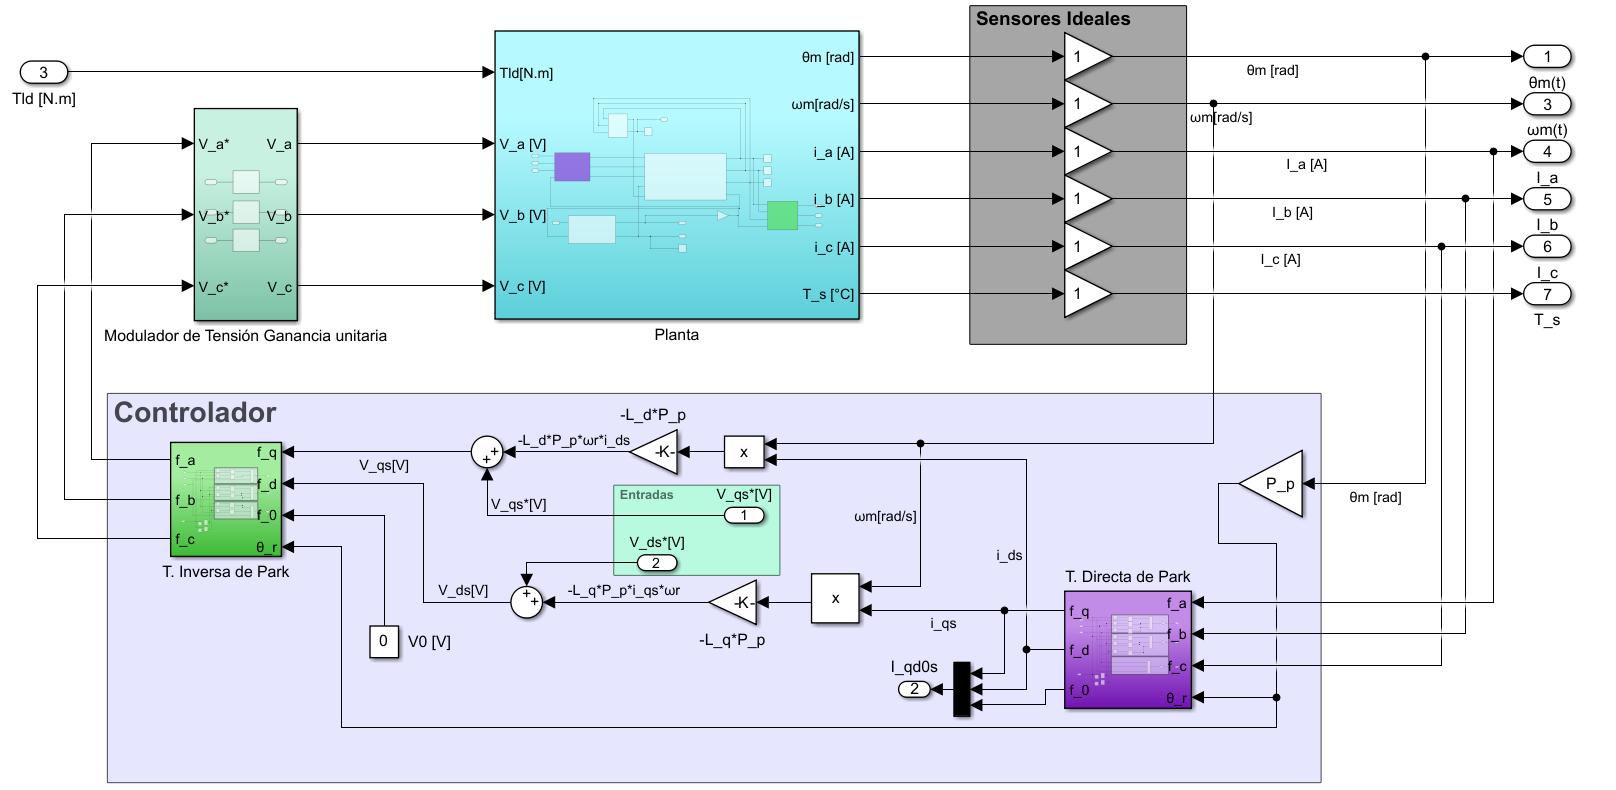
\includegraphics[width=\linewidth,height=0.9\textheight,keepaspectratio]{imagenes/NL con realimentacion NL.png}

\end{frame}

% -------------------------------------------------------------------
%  SLIDE 53 - Comparación conceptual
% -------------------------------------------------------------------
\begin{frame}{LPV vs. LTI aumentado: comparación conceptual}
{\small\color{uncGray}Ambos modelos son lineales en su forma final, pero no representan la misma idea de linealización ni tratan igual las no linealidades físicas del accionamiento.}\par
\vspace{2mm}

\centering
\footnotesize
\renewcommand{\arraystretch}{1.25}
\resizebox{\textwidth}{!}{%
\begin{tabular}{|>{\bfseries}p{0.18\textwidth}|p{0.41\textwidth}|p{0.41\textwidth}|}
\hline
\multicolumn{1}{|c|}{\color{uncBlue}\textbf{Aspecto}} &
\multicolumn{1}{c|}{\color{uncBlue}\textbf{LPV (pequeñas señales)}} &
\multicolumn{1}{c|}{\color{uncBlue}\textbf{LTI aumentado (realim.\ NL)}} \\
\hline\hline
Naturaleza de la linealización &
Expansión en Taylor truncada a 1\textsuperscript{er} orden (\emph{pequeña señal}). Sólo válida cerca de $(x_o,u_o)$. &
Algebraicamente exacto, sin Taylor. Cancela las NL inyectando tensiones virtuales calculadas dinámicamente. \\
\hline
Carga gravitacional (NL mecánica) &
Linealiza $\sin(\theta_{m,o}/r)\to$ rigidez local. Aparece $A_{2,1}\propto\cos(\theta_{m,o}/r)$: los polos mecánicos \textbf{cambian con la posición} del brazo. &
Agrupa el término gravitatorio completo dentro de la perturbación total $T_l(t)$. La matriz $A_{2,1}=0$ permanece \textbf{invariante}. \\
\hline
Subsistema térmico &
Conserva la influencia: $R_{s,o}$ depende del equilibrio térmico $T_{s,o}^\circ$ del Jacobiano. &
\textbf{Desacople térmico completo}: $R_s$ se trata como constante rígida en el transitorio rápido. \\
\hline
Estructura al forzar $i_{ds,o}^{r}\equiv 0$ &
Caso particular: el acoplamiento cruzado se vuelve puramente $\lambda'^r_m$ (sin reluctancia), coincidiendo con $A_{3,2}$ del LTI. &
\textbf{Es} el caso ideal de un LPV operando perpetuamente en $i_{ds,o}^{r}=0$ con la gravedad agrupada en $T_l(t)$. \\
\hline
\end{tabular}%
}

\vspace{2mm}
{\scriptsize \textbf{Conclusión:} ambos modelos son comparables pero no equivalentes en su origen. El LTI aumentado puede interpretarse como el caso ideal del LPV con $i_{ds,o}^{r}\equiv 0$ y la gravedad agrupada en la entrada exógena $T_l(t)$.}
\end{frame}

\subsection{Variaciones de corriente en eje d}
% -----------------------------------------------------------

% -------------------------------------------------------------------
%  SLIDE 55 - ids como parametro
% -------------------------------------------------------------------
\begin{frame}{Corriente de eje $d$ como parámetro}
{\small\color{uncGray}Al liberar la condición $i_{ds,o}^{r}=0$, la corriente directa deja de ser solo un estado residual y pasa a modificar la capacidad estática de torque y la dinámica local del modelo LPV.}\par
\vspace{3mm}

\textbf{Torque electromagnético en operación estacionaria:}
\begin{equation*}
T_m=\frac{3}{2}P_p\Big[\lambda'^r_m+(L_d-L_q)i_{ds,o}^{r}\Big]I_{qs,o}^{r}
\end{equation*}

\textbf{Qué cambia respecto del caso base:}
\begin{itemize}
  \item Con $i_{ds,o}^{r}=0$, el torque queda asociado al flujo de los imanes y a $I_{qs,o}^{r}$.
  \item Con $i_{ds,o}^{r}\neq 0$, aparece el aporte de reluctancia por saliencia.
  \item El mismo parámetro desplaza los autovalores del Jacobiano LPV.
\end{itemize}

{\small Esta es una lectura local del LPV: no reemplaza al LTI aumentado, sino que muestra cómo cambia el modelo alrededor de otros puntos de operación.}
\end{frame}

% -------------------------------------------------------------------
%  SLIDE 56 - Reforzamiento y debilitamiento
% -------------------------------------------------------------------
\figslide{Reforzamiento y debilitamiento de campo}{%
La inyección de corriente en eje $d$ altera el flujo magnético total. \textbf{$i_{ds,o}^{r}>0$ (reforzamiento):} aumenta el flujo efectivo y suma torque de reluctancia si $L_d>L_q$. \textbf{$i_{ds,o}^{r}<0$ (debilitamiento):} reduce el flujo efectivo y la fuerza contraelectromotriz; permite mayor velocidad antes de saturar tensión, al costo de menor torque para el mismo $I_{qs,o}^{r}$.%
}{polosaliente_cilindrico.png}{Diagrama representativo de un rotor genérico de polos no salientes y un rotor de polos salientes.}

% -------------------------------------------------------------------
%  SLIDE 57 - Migración con ids
% -------------------------------------------------------------------
% \begin{frame}{Migración dinámica con $i_{ds,o}^{r}$}
% {\small\color{uncGray}Barrido de los autovalores del Jacobiano LPV ante variación de $i_{ds,o}^{r}$, manteniendo el resto del punto de operación nominal. Se reproducen las dos tablas presentadas en el informe (sección 5.1.2.d).}\par
% \vspace{2mm}

% \centering
% \scriptsize
% \textbf{Debilitamiento de campo ($i_{ds,o}^r<0$)}\par\vspace{1mm}
% \begin{tabular}{|c|c|c|c|c|}
% \hline
% $i_{ds,o}^r$ [A] & $\lambda_1$ & $\lambda_2$ & $\lambda_{3,4}$ & $\lambda_5$ \\
% \hline
% $-1{,}2$ & $-1275{,}00$ & $-141{,}30$ & $-94{,}74 \pm j\,23{,}38$ & $-0{,}2657$ \\
% $-1{,}0$ & $-1275{,}00$ & $-145{,}62$ & $-92{,}61 \pm j\,47{,}75$ & $-0{,}2261$ \\
% $-0{,}8$ & $-1275{,}00$ & $-147{,}64$ & $-91{,}62 \pm j\,62{,}75$ & $-0{,}1963$ \\
% $-0{,}6$ & $-1275{,}00$ & $-148{,}88$ & $-91{,}01 \pm j\,74{,}74$ & $-0{,}1731$ \\
% $-0{,}4$ & $-1275{,}00$ & $-149{,}74$ & $-90{,}59 \pm j\,85{,}10$ & $-0{,}1544$ \\
% \hline
% \end{tabular}

% \vspace{2mm}
% \textbf{Reforzamiento de campo ($i_{ds,o}^r>0$)}\par\vspace{1mm}
% \begin{tabular}{|c|c|c|c|c|}
% \hline
% $i_{ds,o}^r$ [A] & $\lambda_1$ & $\lambda_2$ & $\lambda_{3,4}$ & $\lambda_5$ \\
% \hline
% $+0{,}2$ & $-1275{,}00$ & $-151{,}25$ & $-89{,}85 \pm j\,111{,}05$ & $-0{,}1157$ \\
% $+0{,}4$ & $-1275{,}00$ & $-151{,}57$ & $-89{,}70 \pm j\,118{,}65$ & $-0{,}1066$ \\
% $+0{,}6$ & $-1275{,}00$ & $-151{,}83$ & $-89{,}57 \pm j\,125{,}90$ & $-0{,}0986$ \\
% $+0{,}8$ & $-1275{,}00$ & $-152{,}05$ & $-89{,}46 \pm j\,132{,}85$ & $-0{,}0917$ \\
% $+1{,}0$ & $-1275{,}00$ & $-152{,}24$ & $-89{,}37 \pm j\,139{,}56$ & $-0{,}0857$ \\
% \hline
% \end{tabular}
% \normalsize

% \vspace{1mm}
% \raggedright
% {\scriptsize \textbf{Conclusiones del barrido:}
% (i) la parte imaginaria de $\lambda_{3,4}$ crece monotónicamente con $i_{ds,o}^{r}$ $\Rightarrow$ aumenta $\omega_n$ electromecánica;
% (ii) la parte real de $\lambda_{3,4}$ se mantiene en torno a $-91$~rad/s $\Rightarrow$ el amortiguamiento absoluto no se degrada;
% (iii) $\lambda_1$ (eléctrico rápido) y los modos restantes permanecen invariantes o varían levemente.}
% \end{frame}

% -------------------------------------------------------------------
%  SLIDE 58 - Mapa migración de polos LPV con I_ds (parte 1)
% -------------------------------------------------------------------
\figslide{Mapa de migración de polos con $i_{ds,o}^{r}$ --- vista global}{%
Representación gráfica de la migración de los autovalores del Jacobiano LPV en el plano $s$ al barrer $i_{ds,o}^{r}$. La vista global permite apreciar simultáneamente todos los modos: el polo real rápido en $\lambda_1 \approx -1299{,}86$, los polos reales $\lambda_2$ y $\lambda_5$, y el par complejo electromecánico $\lambda_{3,4}$ que es el que más migra.%
}{migracion_ids_1.png}{Mapa de migración de polos del modelo LPV al variar $i_{ds,o}^{r}$: vista global del plano $s$.}

% -------------------------------------------------------------------
%  SLIDE 59 - Mapa migración de polos LPV con I_ds (parte 2 - zoom)
% -------------------------------------------------------------------
\figslide{Mapa de migración de polos con $i_{ds,o}^{r}$ --- zoom}{%
Zoom sobre el par complejo conjugado $\lambda_{3,4}$, donde el barrido de $i_{ds,o}^{r}$ desde el debilitamiento (parte inferior) hacia el reforzamiento (parte superior) se traduce en un crecimiento monotónico de la parte imaginaria, manteniendo la parte real prácticamente invariante en torno a $-91$~rad/s.%
}{migracion_ids_2.png}{Mapa de migración de polos del modelo LPV al variar $i_{ds,o}^{r}$: zoom sobre los polos electromecánicos.}


\subsection{Funciones de Transferencia}

\StartProjectSection{8}{\SecAnalisisLTI}
% -------------------------------------------------------------------
%  SLIDE 60 - Planteo de funciones de transferencia
% -------------------------------------------------------------------
\begin{frame}{Funciones de transferencia del LTI aumentado}
{\small\color{uncGray}A partir del modelo LTI aumentado se buscan las relaciones entrada-salida desde $v_{qs}$ y $T_{ld}$ hacia la posición $\theta_m$.}\par
\vspace{3mm}

\textbf{Condiciones usadas para obtenerlas:}
\begin{itemize}
  \item Modelo incremental con $\bm{x}_{aug}(0)=\bm{0}$.
  \item Resistencia constante: $R_s=R_{s0}$.
  \item La gravedad se agrupa dentro de la perturbación mecánica total $T_l(t)$, fuera de la matriz $\bm{A}_{aug}$.
  \item Como $i_{ds}^{r}$ queda desacoplado, la relación entrada-salida se obtiene con el subsistema nominal de tercer orden.
\end{itemize}

\begin{equation*}
G(s)=\bm{C}\,(s\bm{I}-\bm{A})^{-1}\bm{B}
\end{equation*}
\end{frame}

% -------------------------------------------------------------------
%  SLIDE 61 - Funciones de transferencia finales
% -------------------------------------------------------------------
\begin{frame}{Funciones de transferencia obtenidas}
{\small\color{uncGray}Ambas funciones comparten el mismo denominador de tercer orden. El factor asociado a $i_{ds}^{r}$ no aparece en la relación entrada-salida.}\par
\vspace{2mm}

\small
\begin{equation*}
\Delta_3(s)=
s^3+
\left(\frac{b_{eq}}{J_{eq}}+\frac{R_{s0}}{L_q}\right)s^2+
\left(\frac{b_{eq}R_{s0}}{J_{eq}L_q}+
\frac{3P_p^2{\lambda'^r_m}^{\,2}}{2J_{eq}L_q}\right)s
\end{equation*}

\vspace{2mm}
\resizebox{\textwidth}{!}{$
G_1(s)=\frac{\Theta_m(s)}{V_{qs}(s)}
=
\frac{\dfrac{3P_p\lambda'^r_m}{2J_{eq}L_q}}{\Delta_3(s)}
\qquad\qquad
G_2(s)=\frac{\Theta_m(s)}{T_l(s)}
=
\frac{-\dfrac{1}{rJ_{eq}}\left(s+\dfrac{R_{s0}}{L_q}\right)}{\Delta_3(s)}
$}
\normalsize


\end{frame}



% -------------------------------------------------------------------
%  SLIDE 62 - Estabilidad a lazo abierto
% -------------------------------------------------------------------
\begin{frame}{Autovalores y estabilidad a lazo abierto}
{\small\color{uncGray}El polinomio característico del modelo aumentado separa el integrador de posición, el modo electromecánico y el modo residual del eje $d$.}\par
\vspace{1.5mm}

\definitionbox{Estabilidad del subsistema físico}{Los modos asociados a las variables que almacenan energía o representan dinámica propia del accionamiento deben tener parte real negativa. La posición se interpreta como una coordenada cinemática acumulada.}
\vspace{1mm}

{\small
\begin{equation*}
\det(s\bm{I}-\bm{A}_{aug})=
\underbrace{\left(s+\frac{R_{s0}}{L_d}\right)}_{\lambda_4}
\underbrace{s}_{\lambda_1}
\underbrace{\left(s^2+a_2s+a_1\right)}_{\lambda_{2,3}}
\end{equation*}
}

\small
\textbf{Valores nominales:}
\begin{itemize}
  \item $\lambda_1=0$: integrador cinemático de posición; no representa almacenamiento de energía.
  \item $\lambda_{2,3}=-91{,}7\pm j\,148{,}0$: modo electromecánico subamortiguado, $\zeta\simeq0{,}527$.
  \item $\lambda_4=-160{,}3$: dinámica residual de $i_{ds}^{r}$, con $\tau_d\simeq6{,}24$ ms.
\end{itemize}

\textbf{Conclusión:}
{\small El sistema físico se considera \textbf{estable}. Una entrada constante puede producir una deriva de $\theta_m$ por integración cinemática, pero no una pérdida de estabilidad del subsistema electromecánico.}
\end{frame}

% -------------------------------------------------------------------
%  SLIDE 63 - Mapa polos y ceros
% -------------------------------------------------------------------
\figslide{Mapa de polos y ceros a lazo abierto}{%
El mapa confirma la estructura anterior: un polo cinemático en el origen, el par electromecánico estable y el polo residual de $i_{ds}^{r}$ marcado como cancelado. El polo en el origen no compromete la estabilidad física; justifica cerrar el lazo para regular la coordenada de posición.% 
}{polos_ceros_LA.png}{Mapa de polos y ceros a lazo abierto para ambas funciones de transferencia del modelo LTI aumentado. Se indica con $\times$ roja el polo cancelado de $i_{ds}^r$.}

\subsection{Variaciones paramétricas}
% -------------------------------------------------------------------
%  SLIDE 64 — Variaciones paramétricas
% -------------------------------------------------------------------

% -------------------------------------------------------------------
%  SLIDE 65 - Variacion de Rs
% -------------------------------------------------------------------
\figslide{Migración ante variación de $R_s$}{}{migracion_Rs.png}{Migración de polos y ceros en el plano $s$ (izq.) y variación de $\omega_n$ y $\zeta$ (der.) ante cambios en $R_s$.}

% -------------------------------------------------------------------
%  SLIDE 66 - Variacion de carga
% -------------------------------------------------------------------
\figslide{Migración ante variación de carga}{}{migracion_ml.png}{Migración de polos ante variación de masa de carga $m_l$ (izq.) y variación de $\omega_n$ y $\zeta$ (der.).}


\subsection{Observabilidad y Controlabilidad}
% -------------------------------------------------------------------
%  SLIDE 64 — Observabilidad y Controlabilidad
% -------------------------------------------------------------------
% -------------------------------------------------------------------
%  SLIDE 67 — Propiedades del modelo aumentado
% -------------------------------------------------------------------
\begin{frame}{Observabilidad y Controlabilidad}
{\small\color{uncGray}Después de obtener las funciones de transferencia, conviene volver al espacio de estados para identificar qué estados se pueden observar y controlar con las señales disponibles.}\par
\vspace{2mm}
\begin{columns}[T,onlytextwidth]

\begin{column}{0.49\textwidth}
\definitionbox{Observabilidad}{
$\bm{x}^\star\neq\bm{0}$ es no observable si:
\[
\bm{y}(t)=\bm{C}e^{\bm{A}t}\bm{x}^\star=\bm{0},\quad \forall t\geq0
\]

}
\vspace{2mm}
\begin{itemize}
  \item ¿Puede reconstruirse $\bm{x}_{aug}$ midiendo solo $\theta_m$ o solo $\omega_m$?
\end{itemize}
\end{column}

\begin{column}{0.49\textwidth}
\definitionbox{Controlabilidad}{
Existe $\bm{u}(t)$ en $[0,T]$ tal que:
\[
\bm{x}(0)=\bm{x}_0,\qquad \bm{x}(T)=\bm{0}
\]

}

\vspace{2mm}
\begin{itemize}
  \item ¿Puede actuarse sobre todos los estados usando solo $v_{qs}$?
\end{itemize}
\end{column}

\end{columns}

\end{frame}

% -------------------------------------------------------------------
%  SLIDE 68 - Observabilidad desde theta
% -------------------------------------------------------------------
\begin{frame}{Observabilidad desde posición}
{\small\color{uncGray}Con un sensor de posición, la salida elegida es $\bm{C}_\theta=[\,1\;0\;0\;0\,]$. La cadena cinemática permite recuperar información de velocidad y corriente de eje $q$.}\par
\vspace{3mm}

\begin{equation*}
\mathcal{O}_\theta=
\begin{bmatrix}
\bm{C}_\theta\\
\bm{C}_\theta\bm{A}\\
\bm{C}_\theta\bm{A}^2\\
\bm{C}_\theta\bm{A}^3
\end{bmatrix},
\qquad
\operatorname{rango}(\mathcal{O}_\theta)=3<4
\end{equation*}

\textbf{Resultado:}
\begin{itemize}
  \item $\theta_m$ se mide directamente.
  \item $\omega_m$ aparece como derivada de $\theta_m$.
  \item $i_{qs}^r$ se manifiesta por el acoplamiento electromecánico.
  \item $i_{ds}^{r}$ no aparece: no acopla con la salida.
\end{itemize}
\end{frame}

% -------------------------------------------------------------------
%  SLIDE 69 - Observabilidad desde velocidad
% -------------------------------------------------------------------
\begin{frame}{Observabilidad desde velocidad}
{\small\color{uncGray}Si se mide solo velocidad, la salida pasa a ser $\bm{C}_\omega=[\,0\;1\;0\;0\,]$. Esta medición pierde información estructural respecto del sensor de posición.}\par
\vspace{3mm}

\begin{equation*}
\mathcal{O}_\omega=
\begin{bmatrix}
\bm{C}_\omega\\
\bm{C}_\omega\bm{A}\\
\bm{C}_\omega\bm{A}^2\\
\bm{C}_\omega\bm{A}^3
\end{bmatrix},
\qquad
\operatorname{rango}(\mathcal{O}_\omega)=2<4
\end{equation*}

\textbf{Estados no observables:}
\begin{itemize}
  \item $\theta_m$: la velocidad no contiene la condición inicial de posición.
  \item $i_{ds}^{r}$: sigue siendo un modo interno desacoplado.
\end{itemize}

\vspace{3mm}
{\small \textbf{Conclusión:} No se requiere un sensor de velocidad, simplemente con un sensor de posición es posible estimar la velocidad.}
\end{frame}

% -------------------------------------------------------------------
%  SLIDE 70 - Controlabilidad desde vqs
% -------------------------------------------------------------------
\begin{frame}{Controlabilidad desde $v_{qs}$}
{\small\color{uncGray}La entrada lineal de control actúa directamente sobre la corriente de eje $q$ y desde allí se propaga hacia la velocidad y la posición.}\par
\vspace{3mm}

\begin{equation*}
\mathcal{C}_{v_q}=
\begin{bmatrix}
\bm{B}_c & \bm{A}\bm{B}_c & \bm{A}^2\bm{B}_c & \bm{A}^3\bm{B}_c
\end{bmatrix},
\qquad
\operatorname{rango}(\mathcal{C}_{v_q})=3<4
\end{equation*}

\textbf{Estado no controlable desde $v_{qs}$:}
\begin{itemize}
  \item $i_{ds}^{r}$, porque la cuarta fila queda desacoplada y $B_c(4)=0$.
\end{itemize}
\end{frame}

% -------------------------------------------------------------------
%  SLIDE 71 - Entrada adicional vds
% -------------------------------------------------------------------
\begin{frame}{Entrada adicional en eje $d$}
{\small\color{uncGray}El estado $i_{ds}^{r}$ podría controlarse agregando la tensión de eje directo como segunda entrada manipulable.}\par
\vspace{2mm}

\begin{equation*}
\bm{B}_{ext}=
\begin{bmatrix}
0 & 0\\
0 & 0\\
\frac{1}{L_q} & 0\\
0 & \frac{1}{L_d}
\end{bmatrix},
\qquad
\operatorname{rango}(\mathcal{C}_{ext})=4
\end{equation*}

\textbf{Interpretación:}
\begin{itemize}
  \item Matemáticamente, $v_{ds}^{r}$ completa la controlabilidad del modelo aumentado.
  \item En la estrategia adoptada, esa tensión ya se usa por la ley mínima para forzar $i_{ds}^{r}\to0$.
  \item No se trata de un grado de libertad libre para el control externo de posición.
\end{itemize}
\end{frame}

% ===================================================================
%  BLOQUE — Simulación Dinámica
%  (señales, Simulink, theta_m, omega_m, i_qs con errores)
% ===================================================================

\StartProjectSection{9}{\SecDinamica}
\subsection{Simulación dinámica NL vs LTI aumentado}
% -------------------------------------------------------------------
%  SLIDE 73 -- Simulación Dinámica: Modelo NL vs LTI Aumentado
% -------------------------------------------------------------------

% -------------------------------------------------------------------
%  SLIDE 74 — Planteo de la simulación
% -------------------------------------------------------------------
\begin{frame}{Planteo de la simulación}
{\small\color{uncGray}Se compara el modelo no lineal completo (6 estados) con las leyes de control NL de desacoplamiento mínima y complementaria contra el modelo LTI aumentado (4 estados), implementados en MATLAB/Simulink.}\par
\vspace{4mm}

\textbf{Condiciones del ensayo:}
\begin{itemize}
\item Tres condiciones iniciales: $i_{ds}^{r}(0) \in \{\,0,\;+0{,}5,\;-0{,}5\,\}$~A.
\item Resto del estado inicial en cero: $\theta_m(0) = \omega_m(0) = i_{qs}^{r}(0) = 0$.
\item Temperatura ambiente $T_{amb}^\circ = 25\,^\circ$C.
\item Las dos señales de excitación se aplican simultáneamente al modelo NL y al LTI aumentado en paralelo.
\end{itemize}
\end{frame}

% -------------------------------------------------------------------
%  SLIDE 75 — Señales de excitación (ecuaciones cases)
% -------------------------------------------------------------------
\begin{frame}{Señales de excitación}
{\small\color{uncGray}La consigna define una secuencia temporal de 10 eventos (escalones) que producen transitorios sucesivos. La combinación de ambas señales permite explorar los cuatro cuadrantes de operación.}\par
\vspace{2mm}

\begin{columns}[T]
\column{0.49\textwidth}
\textbf{Pulso de tensión en eje $q$:}
\footnotesize
\[
v_{qs}^{r*}(t) = \begin{cases}
0~\text{V} & t < 0{,}1~\text{s} \\
+19{,}596~\text{V} & 0{,}1 \leq t < 0{,}7~\text{s} \\
0~\text{V} & 0{,}7 \leq t < 1{,}1~\text{s} \\
-19{,}596~\text{V} & 1{,}1 \leq t < 1{,}7~\text{s} \\
0~\text{V} & t \geq 1{,}7~\text{s}
\end{cases}
\]
\normalsize

\column{0.49\textwidth}
\textbf{Doble pulso de torque de carga:}
\footnotesize
\[
T_{ld}(t) = \begin{cases}
0 & t < 0{,}3~\text{s} \\
+6{,}28~\text{N$\cdot$m} & 0{,}3 \leq t < 0{,}5~\text{s} \\
-6{,}28~\text{N$\cdot$m} & 0{,}5 \leq t < 0{,}9~\text{s} \\
0 & 0{,}9 \leq t < 1{,}3~\text{s} \\
+6{,}28~\text{N$\cdot$m} & 1{,}3 \leq t < 1{,}5~\text{s} \\
-6{,}28~\text{N$\cdot$m} & 1{,}5 \leq t < 1{,}9~\text{s} \\
0 & t \geq 1{,}9~\text{s}
\end{cases}
\]
\normalsize
\end{columns}
\end{frame}

% -------------------------------------------------------------------
%  SLIDE 76 — Figura señales de excitación combinadas
% -------------------------------------------------------------------
\figslide{Señales de excitación combinadas}{%
10 transitorios consecutivos separados por instantes $t_1=0{,}1$~s, $t_2=0{,}3$, $t_3=0{,}5$, $t_4=0{,}7$, $t_5=0{,}9$, $t_6=1{,}1$, $t_7=1{,}3$, $t_8=1{,}5$, $t_9=1{,}7$, $t_{10}=1{,}9$~s. Trans.~1--5 corresponden al pulso positivo de $v_{qs}^{r*}$ y Trans.~6--10 a su simétrico negativo.%
}{sim_senales_entrada.png}{Señales de excitación: consigna de tensión $v_{qs}^{r*}(t)$ y torque de carga $T_{ld}(t)$.}

% -------------------------------------------------------------------
%  SLIDE 77 — Modelo en Simulink
% -------------------------------------------------------------------
\figslide{Modelo en Simulink}{%
Modelo en Simulink con dos subsistemas en paralelo: NL completo (6 estados) y LTI aumentado (4 estados), ambos excitados por las mismas señales $v_{qs}^{r*}(t)$ y $T_{ld}(t)$.%
}{sim_diagrama_bloques.png}{Diagrama de bloques en Simulink: modelo NL desacoplado y LTI aumentado en paralelo frente al mismo $v_q^*$ consigna y torque de perturbación.}

% -------------------------------------------------------------------
%  SLIDE 78 — Sub-ítem a: caso nominal i_ds(0)=0
% -------------------------------------------------------------------
\begin{frame}{Respuesta del estado interno — Sub-ítem a: caso nominal $i_{ds}^{r}(0) = 0$~A}
{\small\color{uncGray}Resultados para el caso nominal comparando NL (6 estados) vs LTI aumentado (4 estados). Los efectos de $i_{ds}^{r}(0)\neq 0$ se analizan por separado en el Sub-ítem~c.}\par
\vspace{4mm}

\textbf{Parámetros del modelo LTI aumentado:}
\begin{itemize}
\item Temperatura ambiente $T_{amb}^\circ = 25\,^\circ$C.
\item Resistencia constante $R_s = R_{s0} = 1{,}058~\Omega$, evaluada a la temperatura media de operación del estator ($\sim 29{,}5\,^\circ$C).
\item No se usa $R_{sREF} = 1{,}02~\Omega$ a $20\,^\circ$C: el valor adoptado es consistente con el desacoplamiento térmico del modelo lineal.
\end{itemize}
\end{frame}

% -------------------------------------------------------------------
%  SLIDE 79 — Posición angular theta_m
% -------------------------------------------------------------------
\figslide{Posición angular $\theta_m(t)$}{%
$\theta_m$ crece como rampa durante los pulsos de tensión, consecuencia directa del integrador puro $\dot{\theta}_m = \omega_m$. Alcanza un máximo $\approx 242$~rad en $t \approx 0{,}7$~s, se mantiene durante $v_{qs}^{r*} = 0$ y retorna hacia cero durante el pulso negativo.%
}{sim_theta_m.png}{Posición angular $\theta_m(t)$: comparación NL (azul) vs LTI aumentado (rojo). Panel inferior: señales de excitación ($T_l$ y $v_{qs}^*$). }

% -------------------------------------------------------------------
%  SLIDE 80 — Error de seguimiento en theta_m
% -------------------------------------------------------------------
\figslide{Error de seguimiento en $\theta_m(t)$}{%
Error acotado por debajo de $0{,}21$~rad ($<0{,}1\%$ de la excursión de $242$~rad). No se anula en régimen permanente: exhibe una deriva lenta acumulativa, porque $\theta_m$ es la integral de $\omega_m$ y el integrador acumula las pequeñas discrepancias instantáneas de velocidad. Offset residual $\approx 0{,}05$~rad al final del ensayo. Es comportamiento inherente al integrador puro de la planta, no error de modelado.%
}{sim_theta_m_error.png}{Error de seguimiento en $\theta_m(t)$: diferencia $\theta_m^{NL}-\theta_m^{LTI}$.\textbf{Error relativo $< 0{,}1\%$ de la excursión de 242~rad.}}

% -------------------------------------------------------------------
%  SLIDE 81 — Velocidad angular omega_m
% -------------------------------------------------------------------
\figslide{Velocidad angular $\omega_m(t)$}{%
Gobernada por el modo electromecánico subamortiguado ($\lambda_{2,3} = -91{,}7 \pm j\,148$, $\zeta = 0{,}527$, $\omega_n = 174$~rad/s, del análisis de estabilidad LA). Velocidad de vacío $\approx \pm 405$~rad/s, sobrepico $\approx 14\%$, tiempo de establecimiento ($\pm 1\%$) $\approx 50$~ms. La realimentación back-EMF fusiona los modos eléctrico y mecánico en una resonancia rápida ($\tau \approx 11$~ms); no domina $\tau_m = J_{eq}/b_{eq} \approx 0{,}90$~s.%
}{sim_omega_m.png}{Velocidad angular $\omega_m(t)$: comparación NL (azul) vs LTI aumentado (rojo). Panel inferior: señales de excitación ($T_l$ y $v_{qs}^*$).}

% -------------------------------------------------------------------
%  SLIDE 82 — Error de seguimiento en omega_m
% -------------------------------------------------------------------
\figslide{Error de seguimiento en $\omega_m(t)$}{%
Concordancia NL-LTI excelente: error prácticamente nulo en régimen ($<0{,}5$~rad/s) y picos $\leq 9$~rad/s únicamente en las conmutaciones, que se extinguen en milisegundos.%
}{sim_omega_m_error.png}{Error de seguimiento en $\omega_m(t)$: diferencia $\omega_m^{NL}-\omega_m^{LTI}$. \textbf{Error en régimen $< 0{,}12\%$ vs $\pm 405$~rad/s; picos $\leq 2{,}2\%$ en conmutaciones.}}

% -------------------------------------------------------------------
%  SLIDE 83 — Corriente i_qs
% -------------------------------------------------------------------
\figslide{Corriente de eje $q$, $i_{qs}^r(t)$}{%
Pico de torque transitorio $\approx \pm 10{,}4$~A (no $v_{qs}^{r*}/R_{s0}$) que decae hasta $\approx 0{,}1$~A en régimen, a medida que la FCEM $\lambda'^r_m P_p \omega_m$ equilibra la tensión aplicada. El pico es el valor relevante frente a $I_{s,max} = 2$~A rms (límite ampliamente superado en este ensayo LA). Como $i_{ds}^{r} \equiv 0$, $T_{em} = k_t\,i_{qs}^r$ con $k_t = \tfrac{3}{2}P_p\lambda'^r_m$: la forma de onda de $T_{em}(t)$ es proporcional a $i_{qs}^r(t)$.%
}{sim_iqs.png}{Corriente de eje $q$, $i_{qs}^r(t)$: comparación NL (azul) vs LTI aumentado (rojo). Panel inferior: señales de excitación ($T_l$ y $v_{qs}^{r*}$).}

% -------------------------------------------------------------------
%  SLIDE 84 — Error de seguimiento en i_qs
% -------------------------------------------------------------------
\figslide{Error de seguimiento en $i_{qs}^r(t)$}{%
Los modelos se solapan casi perfectamente: error nulo en régimen y picos $\leq 0{,}26$~A únicamente en las conmutaciones, confirmando que las leyes de control NL linealizan efectivamente la dinámica de la planta.%
}{sim_iqs_error.png}{Error de seguimiento en $i_{qs}^r(t)$: diferencia $i_{qs}^{r,NL}-i_{qs}^{r,LTI}$. \textbf{Error nulo en régimen; picos $\leq 2{,}5\%$ del pico de $\pm 10{,}4$~A en conmutaciones.}}

% ===================================================================
%  BLOQUE — Simulación Dinámica 5.1.6 parte 2
%  (T_s, v_ds, abc, cuadrantes torque-vel, angulo carga, metricas)
% ===================================================================

% -------------------------------------------------------------------
%  SLIDE 85 — Temperatura T_s
% -------------------------------------------------------------------
\figslide{Temperatura del estator $T_s(t)$}{%
$T_s^\circ$ crece levemente respecto de $T_{amb}^\circ=25\,^\circ$C por pérdidas resistivas $P_{s,perd}=\tfrac{3}{2}R_s(i_{qs}^{r\,2}+i_{ds}^{r\,2})$. Cambio mínimo porque la constante térmica $\tau_{th}=R_{ts\text{-}amb}\cdot C_{ts}\approx 120$~s es muy superior a la duración del ensayo ($2{,}2$~s). Justifica la hipótesis LTI de $R_s=R_{s0}$ constante. El LTI aumentado (4 estados) \textbf{no} incluye temperatura como variable de estado.%
}{sim_Ts.png}{Temperatura del estator $T_s^\circ(t)$: comparación modelo NL vs LTI aumentado ($i_{ds}^r(0) = 0$~A).}

% -------------------------------------------------------------------
%  SLIDE 86 — Tensión v_ds de la ley de control mínima
% -------------------------------------------------------------------
\figslide{Tensión $v_{ds}(t)$ de la ley de control mínima}{%
La ley de control mínima impone internamente $v_{ds}=-L_q\,i_{qs}\,\omega_r$, proporcional al producto $i_{qs}\cdot\omega_m$. Esta tensión es no nula solo cuando ambas variables lo son simultáneamente, y su magnitud crece con el nivel de operación del sistema.%
}{sim_v_ds.png}{Tensión $v_{ds}$ del modelo NL ($i_{ds}^r(0) = 0$~A).}

% -------------------------------------------------------------------
%  SLIDE 87 — Corrientes en coordenadas abc
% -------------------------------------------------------------------
\figslide{Corrientes de fase $i_a$, $i_b$, $i_c$ (Park inversa)}{%
Reconstrucción mediante la Transformación Inversa de Park: $[i_a,i_b,i_c]^T = \bm{T}_{dq0}^{-1}(\theta_e)\,[i_{ds}^{r},i_{qs},i_{0s}]^T$, con $\theta_e = P_p\cdot\theta_m$. Las ondas son senoidales moduladas en amplitud con frecuencia eléctrica $\omega_e = P_p\cdot\omega_m$ proporcional a la velocidad del rotor. Si $\omega_m=0$ las corrientes $abc$ son constantes (frecuencia eléctrica nula).%
}{sim_corrientes_abc.png}{Corrientes de fase $i_a$, $i_b$, $i_c$ obtenidas por Transformación Inversa de Park (modelo NL, $i_{ds}^r(0) = 0$~A).}

% -------------------------------------------------------------------
%  SLIDE 88 — Curva paramétrica torque vs velocidad
% -------------------------------------------------------------------
\figslide{Curva paramétrica $T_{em}(\omega_m)$: cuadrantes de operación}{%
Trayectoria construida con los datos del script MATLAB, segmentada en los 10 transitorios que conectan los puntos de (cuasi-)equilibrio $P_0$ a $P_{10}$. Cada transitorio se distingue por color; las flechas indican el sentido de recorrido; los diamantes marcan los puntos de equilibrio.%
}{sim_torque_vs_velocidad.png}{Torque electromagnético vs velocidad angular: cuadrantes de operación del PMSM. Cada transitorio en color, flechas de sentido y diamantes en los equilibrios $P_0$ a $P_{10}$.}

% -------------------------------------------------------------------
%  SLIDE 89 — Ángulo de carga: definición
% -------------------------------------------------------------------
\begin{frame}{Ángulo de carga $\delta(t)$: definición}
{\small\color{uncGray}Desfasaje electromagnético entre el ángulo eléctrico de la referencia (tensión $v_{as}$) y la posición eléctrica del rotor $\theta_r$. La tensión de fase $a$ se usa como referencia angular porque su posición es constante en estado estacionario.}\par
\vspace{3mm}

\textbf{Definición:}
\begin{equation*}
\delta(t) \equiv \theta_{ev}(t) - \theta_r(t) = \int_{0}^{t}\!\big[\,\omega_e(\xi) - \omega_r(\xi)\,\big]\,d\xi \;+\; \big[\,\theta_{ev}(0) - \theta_r(0)\,\big]
\end{equation*}

\textbf{donde:}
\begin{itemize}
\item $\omega_e$: velocidad angular de la referencia (tensión de fase $a$).
\item $\omega_r$: velocidad angular eléctrica del rotor.
\end{itemize}

\vspace{2mm}
{\small Se asumen posiciones angulares iniciales nulas para ambas variables.}
\end{frame}

% -------------------------------------------------------------------
%  SLIDE 90 — Cálculo de theta_ev: Clarke + atan2
% -------------------------------------------------------------------
\begin{frame}{Cálculo de $\theta_{ev}$: Clarke + atan2}
{\small\color{uncGray}A partir de las tensiones senoidales de fase, la Transformación de Clarke proyecta al plano $\alpha$-$\beta$ y la función atan2 recupera el ángulo eléctrico instantáneo de la referencia.}\par
\vspace{2mm}

\textbf{Tensiones de fase senoidales:}
\begin{align*}
v_{as}(t) &\approx \sqrt{2}\,\frac{V_{sl}(t)}{\sqrt{3}}\cos\!\big(\theta_{ev}(t)\big) \\
v_{bs}(t) &\approx \sqrt{2}\,\frac{V_{sl}(t)}{\sqrt{3}}\cos\!\big(\theta_{ev}(t) - \tfrac{2\pi}{3}\big) \\
v_{cs}(t) &\approx \sqrt{2}\,\frac{V_{sl}(t)}{\sqrt{3}}\cos\!\big(\theta_{ev}(t) + \tfrac{2\pi}{3}\big)
\end{align*}

\textbf{Transformación de Clarke} (proyección $\alpha$-$\beta$):
\begin{align*}
v_\alpha(t) &= \tfrac{2}{3}\!\big(v_{as}(t) - \tfrac{1}{2}v_{bs}(t) - \tfrac{1}{2}v_{cs}(t)\big)
= \sqrt{2}\,\tfrac{V_{sl}(t)}{\sqrt{3}}\cos\theta_{ev}(t)\\
v_\beta(t) &= \tfrac{\sqrt{3}}{3}\!\big(v_{bs}(t) - v_{cs}(t)\big)
= \sqrt{2}\,\tfrac{V_{sl}(t)}{\sqrt{3}}\sin\theta_{ev}(t)
\end{align*}

\textbf{Recuperación del ángulo:}
\begin{equation*}
\theta_{ev}(t) = \mathrm{atan2}\!\big(v_\beta(t),\,v_\alpha(t)\big)
\end{equation*}
\end{frame}

% -------------------------------------------------------------------
%  SLIDE 91 — Figura ángulo de carga
% -------------------------------------------------------------------
\figslide{Ángulo de carga $\delta(t)$}{%
Evolución de $\delta(t)$ del modelo NL para $i_{ds}^{r}(0)=0$~A. Refleja directamente la diferencia integrada entre $\omega_e$ (referencia eléctrica) y $\omega_r$ (rotor) a lo largo de la secuencia de transitorios aplicada.%
}{sim_angulo_carga.png}{Ángulo de carga $\delta(t)$ vs $t$ (modelo NL, $i_{ds}^r(0) = 0$~A).}

% -------------------------------------------------------------------
%  SLIDE 92 — Métricas de transitorio (planteo)
% -------------------------------------------------------------------
\begin{frame}{Métricas de transitorio}
{\small\color{uncGray}Se determinan las métricas de los 10 transitorios para el caso nominal $i_{ds}^{r}(0)=0$~A del modelo LTI aumentado.}\par
\vspace{4mm}

\textbf{Variable subamortiguada:} $\omega_m$, gobernada por el par de polos complejos $\zeta=0{,}527$, $\omega_n=174$~rad/s del análisis de estabilidad LA.

\textbf{Métricas medidas sobre $\omega_m$:}
\begin{itemize}
\item $\omega_{m,ss}$: velocidad de régimen del segmento.
\item $M_p$: sobrepico.
\item $t_p$: tiempo de pico.
\item $t_r$: tiempo de crecimiento (10--90 \%).
\item $t_s$: tiempo de establecimiento ($\pm 1$~\%).
\end{itemize}

\textbf{Métricas sobre $i_{qs}$:} pico y valor de régimen.

\end{frame}

% -------------------------------------------------------------------
%  SLIDE 93 — Tabla de métricas (10 transitorios)
% -------------------------------------------------------------------
\begin{frame}{Tabla de métricas --- 10 transitorios}
{\small\color{uncGray}Modelo LTI aumentado, $i_{ds}^{r}(0)=0$~A. $M_p$, $t_p$, $t_r$ y $t_s$ medidos sobre $\omega_m$.}\par
\vspace{2mm}

\centering
\scriptsize
\renewcommand{\arraystretch}{1.1}
\begin{tabular}{|c|l|r|r|r|r|r|r|r|}
\hline
\textbf{Tr.} & \textbf{Evento} & $\omega_{m,ss}$ & $M_p$ & $t_p$ & $t_r$ & $t_s$ & $i_{qs}^{r,\text{pico}}$ & $i_{qs}^{r,\text{reg}}$ \\
 & & [rad/s] & [\%] & [ms] & [ms] & [ms] & [A] & [A] \\
\hline
1 & $v_{qs}^{r*}\to+19{,}6$~V & $405{,}5$ & $14{,}3$ & $21{,}3$ & $9{,}7$ & $50{,}1$ & $10{,}39$ & $0{,}12$ \\
2 & $T_{ld}\to+6{,}28$~Nm & $389{,}6$ & $25{,}6$ & $14{,}4$ & $5{,}8$ & $45{,}7$ & $0{,}95$ & $0{,}85$ \\
3 & $T_{ld}\to-6{,}28$~Nm & $421{,}4$ & $25{,}6$ & $14{,}3$ & $5{,}8$ & $45{,}7$ & $0{,}85$ & $-0{,}60$ \\
4 & $v_{qs}^{r*}\to 0$~V & $15{,}9$ & $14{,}3$ & $21{,}3$ & $9{,}7$ & $50{,}1$ & $-10{,}99$ & $-0{,}72$ \\
5 & $T_{ld}\to 0$~Nm & $0{,}0$ & $25{,}6$ & $14{,}3$ & $5{,}8$ & $45{,}7$ & $-0{,}72$ & $0{,}00$ \\
6 & $v_{qs}^{r*}\to-19{,}6$~V & $-405{,}5$ & $14{,}3$ & $21{,}2$ & $9{,}7$ & $50{,}1$ & $-10{,}39$ & $-0{,}12$ \\
7 & $T_{ld}\to+6{,}28$~Nm & $-421{,}4$ & $25{,}6$ & $14{,}4$ & $5{,}8$ & $45{,}7$ & $0{,}70$ & $0{,}60$ \\
8 & $T_{ld}\to-6{,}28$~Nm & $-389{,}6$ & $25{,}6$ & $14{,}4$ & $5{,}8$ & $45{,}7$ & $-1{,}05$ & $-0{,}85$ \\
9 & $v_{qs}^{r*}\to 0$~V & $15{,}9$ & $14{,}3$ & $21{,}3$ & $9{,}7$ & $50{,}1$ & $9{,}55$ & $-0{,}72$ \\
10 & $T_{ld}\to 0$~Nm & $0{,}0$ & $25{,}6$ & $14{,}4$ & $5{,}8$ & $45{,}7$ & $-0{,}72$ & $0{,}00$ \\
\hline
\end{tabular}
\normalsize

\vspace{2mm}
{\scriptsize $\omega_{m,ss}$: velocidad de régimen del segmento. $i_{qs}^{r,\text{pico}}$/$i_{qs}^{r,\text{reg}}$: valor pico y de régimen de la corriente de eje $q$.}
\end{frame}

% ===================================================================
%  BLOQUE — Simulación Dinámica 5.1.6 parte 3
%  (Sub-item c: i_ds(0)=±0.5 A + Sub-item d: field forcing/weakening)
% ===================================================================

% -------------------------------------------------------------------
%  SLIDE 94 — Planteo Sub-item c: tres condiciones iniciales
% -------------------------------------------------------------------
\begin{frame}{Efecto de $i_{ds}^{r}(0)$ sobre el sistema}
{\small\color{uncGray}Se compara el comportamiento de $i_{ds}^{r}(t)$ para tres condiciones iniciales en ambos modelos. Objetivo: verificar el desacople efectivo del eje $d$ y justificar el carácter no restrictivo de la hipótesis $i_{ds}^{r}(0)=0$ usada en la linealización.}\par
\vspace{4mm}

\textbf{Condiciones iniciales evaluadas:}
\begin{itemize}
\item $i_{ds}^{r}(0) = 0$~A (caso base, ya analizado en Sub-ítem~a).
\item $i_{ds}^{r}(0) = +0{,}5$~A.
\item $i_{ds}^{r}(0) = -0{,}5$~A.
\end{itemize}

\vspace{2mm}
\textbf{Resto del ensayo invariante:} mismas señales de excitación $v_{qs}^{r*}(t)$ y $T_{ld}(t)$, misma ley de control mínima $v_{ds} = -L_q\,i_{qs}\,\omega_r$, mismo $T_{amb}^\circ=25\,^\circ$C.

Se analiza la evolución de $i_{ds}^{r}(t)$ en NL y LTI y el impacto sobre el resto de las variables de estado.
\end{frame}

% -------------------------------------------------------------------
%  SLIDE 95 — i_ds NL y LTI, tres casos
% -------------------------------------------------------------------
\begin{frame}{$i_{ds}^{r}(t)$ en los modelos NL y LTI}
{\small\color{uncGray}Las trayectorias parten de ${0,,+0{,}5,,-0{,}5}$~A y convergen rápidamente a $i_{ds}^{r}=0$. En el LTI son exponenciales puras de primer orden; el NL presenta el mismo desacoplamiento efectivo.}\par
\vspace{2mm}
\begin{columns}[T,onlytextwidth]
\begin{column}{0.49\textwidth}
\centering

\includegraphics[width=\linewidth,height=0.8\textheight,keepaspectratio]{imagenes/sim_ids_NL_3casos.png}\par
{\scriptsize Modelo no lineal}
\end{column}
\begin{column}{0.49\textwidth}
\centering

\includegraphics[width=\linewidth,height=0.8\textheight,keepaspectratio]{imagenes/sim_ids_LTI_3casos.png}\par
{\scriptsize Modelo LTI aumentado}
\end{column}
\end{columns}
\end{frame}
% -------------------------------------------------------------------
%  SLIDE 97 — Planteo Sub-item d: consigna v_ds*
% -------------------------------------------------------------------
\begin{frame}{Field forcing y Field weakening a lazo abierto}
{\small\color{uncGray}Se agrega una consigna de tensión $v_{ds}^{*}$ sumada a la ley de control mínima, con $i_{ds}^{r}(0)=0$~A para aislar el efecto de la tensión inyectada.}\par
\vspace{2mm}

\textbf{Consigna agregada a la ley mínima:}
\begin{equation*}
v_{ds}(t) = \underbrace{-L_q\,i_{qs}\,\omega_r}_{\text{ley mínima}} + v_{ds}^{*}(t)
\end{equation*}

\begin{equation*}
v_{ds}^{*}(t) = \begin{cases}
0 & t < 0{,}5~\text{s} \\
+1{,}9596~\text{V} & t \geq 0{,}5~\text{s} \quad \text{(field forcing)}\\
-1{,}9596~\text{V} & t \geq 0{,}5~\text{s} \quad \text{(field weakening)}
\end{cases}
\end{equation*}

\vspace{2mm}
{\small \textbf{Amplitud:} $V_{ds}^{*} = V_{qs,nom}/10 = 1{,}9596$~V, escalón aplicado a partir de $t=0{,}5$~s. $i_{ds}^{r}(0)=0$~A para aislar el efecto de la tensión.}
\end{frame}

% -------------------------------------------------------------------
%  SLIDE 98 — Figura field forcing/weakening
% -------------------------------------------------------------------
\figslide{Efecto del field forcing y field weakening sobre $i_{ds}^{r}(t)$}{%
A partir de $t=0{,}5$~s, $i_{ds}^{r}$ crece exponencialmente hasta $\pm 1{,}92$~A según el signo de la consigna; el caso base ($v_{ds}^{*}=0$) permanece en cero. Comparación de los tres escenarios sobre la misma corriente de eje $d$.%
}{sim_ff_ids.png}{Efecto del field forcing ($v_{ds}^* = +1{,}96$~V) y field weakening ($v_{ds}^* = -1{,}96$~V) sobre $i_{ds}^r(t)$, comparado con el caso base ($v_{ds}^* = 0$).}

% -------------------------------------------------------------------
%  SLIDE 99 — Análisis modelo NL: acoplamientos cruzados
% -------------------------------------------------------------------
\begin{frame}{Análisis del modelo NL: acoplamientos cruzados}
{\small\color{uncGray}El modelo no lineal revela los acoplamientos cruzados que el LTI no representa: la dinámica del eje $d$ depende de $i_{qs}\omega_m$, y el torque incorpora el término de reluctancia $(L_d-L_q)i_{ds}^{r}$.}\par
\vspace{3mm}

\textbf{Dinámica completa del eje $d$ en NL:}
\begin{equation*}
\frac{di_{ds}^{r}}{dt} = \frac{1}{L_d}\!\left[\,v_{ds}^{r}(t) - R_s\,i_{ds}^{r}(t) + L_q\,i_{qs}^{r}(t)\,P_p\,\omega_m(t)\,\right]
\end{equation*}

\textbf{Torque electromagnético con contribución de reluctancia:}
\begin{equation*}
T_m(t) = \tfrac{3}{2}\,P_p\!\left[\,\lambda'^r_m + (L_d - L_q)\,i_{ds}^{r}(t)\,\right]\,i_{qs}^{r}(t)
\end{equation*}

\vspace{2mm}
{\small El signo de $i_{ds}^{r}$ define dos regímenes de operación con efectos opuestos sobre torque, FCEM y velocidad máxima alcanzable.}
\end{frame}

% ===================================================================
%  BLOQUE — 5.2.1 Modulador de Torque
%  (apertura Parte II + desacoplamiento + lazos corriente + consigna torque)
% ===================================================================

\StartProjectSection{10}{\SecControlador}
\subsection{Modulador de torque}
% -------------------------------------------------------------------
%  SLIDE 100 -- Controlador en Cascada
% -------------------------------------------------------------------

% -------------------------------------------------------------------
%  SLIDE 101 — Diseño del Modulador (intro)
% -------------------------------------------------------------------
\begin{frame}{Diseño del Modulador de Torque}
{\small\color{uncGray}Controlador interno vectorial de corriente/torque. Recibe la consigna $T_m^{*}$ del lazo externo y genera las tensiones de comando en coordenadas $qd0$ rotóricas que se envían al inversor.}\par
\vspace{4mm}

\textbf{Estrategia: desacoplamiento completo} de todas las retroalimentaciones físicas naturales de la planta:
\begin{itemize}
\item Acoplamientos magnéticos cruzados entre ejes $q$ y $d$.
\item Fuerzas contraelectromotrices (FCEM) de los imanes.
\item Caídas resistivas variables con la temperatura, $R_s(T_s^\circ)$.
\end{itemize}

\vspace{2mm}
{\small Una vez cancelados estos términos, las corrientes responden a las tensiones de control como integradores puros, lo que habilita controladores P de corriente y una separación clara entre el lazo interno y el externo.}
\end{frame}

% -------------------------------------------------------------------
%  SLIDE 102 — Ecuaciones del rotor a desacoplar
% -------------------------------------------------------------------
\begin{frame}{Ecuaciones del rotor a desacoplar}
{\small\color{uncGray}Recordando las tres ecuaciones de tensión del estator referidas al rotor: contienen $R_s(T_s)$ variable, FCEM de imanes y acoplamientos cruzados $qd$.}\par
\vspace{2mm}

\begin{align*}
v_{qs}^{r} &= R_s(T_s^\circ)\,i_{qs}^{r} + L_q\,\tfrac{d i_{qs}^{r}}{dt} + \big[\lambda'^r_m + L_d\,i_{ds}^{r}\big]\,\omega_r \\[3pt]
v_{ds}^{r} &= R_s(T_s^\circ)\,i_{ds}^{r} + L_d\,\tfrac{d i_{ds}^{r}}{dt} - L_q\,i_{qs}^{r}\,\omega_r \\[3pt]
v_{0s}^{r} &= R_s(T_s^\circ)\,i_{0s} + L_{ls}\,\tfrac{d i_{0s}}{dt}
\end{align*}

\vspace{2mm}
\textbf{Retroalimentaciones físicas naturales identificadas:}
\begin{itemize}
\item Dependencia de $R_s$ con la temperatura $T_s^\circ(t)$.
\item Acoplamiento entre $i_{qs}^{r}$ e $i_{ds}^{r}$ vía $\omega_r$.
\item FCEM proporcional a $\lambda'^r_m\,\omega_r$ en el eje $q$.
\end{itemize}
\end{frame}

% -------------------------------------------------------------------
%  SLIDE 103 — Estrategia: ecuaciones de control propuestas
% -------------------------------------------------------------------
\begin{frame}{Estrategia: ecuaciones de control propuestas}
{\small\color{uncGray}Se proponen tensiones de comando que inyectan términos de compensación (\emph{feedforward}) idénticos a las retroalimentaciones naturales para cancelarlas.}\par
\vspace{2mm}

\begin{align*}
v_{qs}^{r} &= v_{qs}^{r*} + R_s(T_s^\circ)\,i_{qs}^{r} + \big[\lambda'^r_m + L_d\,i_{ds}^{r}\big]\,P_p\,\omega_m \\[3pt]
v_{ds}^{r} &= v_{ds}^{r*} + R_s(T_s^\circ)\,i_{ds}^{r} - L_q\,i_{qs}^{r}\,P_p\,\omega_m \\[3pt]
v_{0s} &= v_{0s}^{*} + R_s(T_s^\circ)\,i_{0s}
\end{align*}

\vspace{2mm}
{\small Las nuevas variables $v_{qd0s}^{r*}$ serán las salidas del lazo proporcional de corriente del próximo slide.}
\end{frame}

% -------------------------------------------------------------------
%  SLIDE 104 — Resultado: dinámica simplificada
% -------------------------------------------------------------------
\begin{frame}{Resultado: dinámica simplificada (integradores puros)}
{\small\color{uncGray}Sustituyendo las tensiones de control propuestas en las ecuaciones de la planta y simplificando, cada eje queda como un integrador puro desacoplado.}\par
\vspace{6mm}

\begin{align*}
v_{qs}^{r*}(t) &= L_q\,\frac{d i_{qs}^{r}(t)}{dt} \\[4pt]
v_{ds}^{r*}(t) &= L_d\,\frac{d i_{ds}^{r}(t)}{dt} \\[4pt]
v_{0s}^{r*}(t) &= L_{ls}\,\frac{d i_{0s}^{r}(t)}{dt}
\end{align*}

\end{frame}

% -------------------------------------------------------------------
%  SLIDE 105 — Figura desacop_realimentacion_fisicas_naturales.png
% -------------------------------------------------------------------
\figslide{Implementación Simulink del desacoplamiento}{%
Implementación en Simulink del desacoplamiento de las retroalimentaciones físicas naturales: las tensiones de referencia $v_{qd0s}^{r*}$ cancelan las caídas resistivas $R_s(T_s^\circ)\,i$, la FCEM y los acoplamientos cruzados entre los ejes $q$ y $d$.%
}{desacop_realimentacion_fisicas_naturales.png}{Implementación en Simulink del desacoplamiento de las retroalimentaciones físicas naturales: cancelación de caídas resistivas, back-EMF y acoplamientos cruzados entre ejes $q$ y $d$.}

% -------------------------------------------------------------------
%  SLIDE 106 — Figura subsistema bloque
% -------------------------------------------------------------------
\figslide{Subsistema equivalente del desacoplamiento}{%
Bloque (subsistema) equivalente del desacoplamiento de retroalimentaciones físicas naturales. Vista empaquetada para integrarlo en el modulador de torque completo.%
}{desacop_realimentacion_fisicas_naturales_bloque.png}{Bloque (subsistema) equivalente del desacoplamiento de retroalimentaciones físicas naturales.}

% -------------------------------------------------------------------
%  SLIDE 107 — Comparación con linealización NL anterior
% -------------------------------------------------------------------
\begin{frame}{Comparación con la linealización implementada hasta el momento}
{\small\color{uncGray}Diferencias respecto a la linealización por retroalimentación NL mínima desarrollada en la etapa inicial a lazo abierto (sección 5.1.2.c).}\par
\vspace{4mm}

\begin{enumerate}
\item \textbf{Generalización del espacio de operación:} se libera la restricción $i_{ds}^{r}\equiv 0$, habilitando \emph{reforzamiento} y \emph{debilitamiento} de campo cuando el rango de tensión del inversor lo requiere.

\item \textbf{Grado de cancelación de dinámicas naturales:} la linealización NL solo cancelaba los acoplamientos cruzados $qd$. El nuevo desacoplamiento cancela \textbf{también} la FCEM de los imanes ($\lambda'^r_m\omega_r$) y las caídas resistivas $R_s(T_s^\circ)\,i$.

\item \textbf{Control explícito de la dinámica de corriente:} permite \textbf{asignar los polos} del lazo interno explícitamente mediante un Modulador de Corriente proporcional, ubicándolos en $p_i = -5000$~rad/s.
\end{enumerate}
\end{frame}

% -------------------------------------------------------------------
%  SLIDE 108 — Planteo R_s(T) vs nominal
% -------------------------------------------------------------------
\begin{frame}{Efecto de $R_s(T_s)$ vs valor nominal constante}
{\small\color{uncGray}¿Cómo tratar la resistencia del estator dentro del modulador de torque, considerando que en la planta real $R_s$ varía con la temperatura por calentamiento Joule?}\par
\vspace{4mm}

\begin{itemize}
\item \textbf{Estimación en línea} con $R_s(T_s(t)) = R_{sREF}\,[\,1 + \alpha_{Cu}(T_s - 20)\,]$ usando el sensor de temperatura: cancelación precisa, robusta frente a cambios térmicos.

\item \textbf{Valor nominal constante} $R_s(25\,^\circ\text{C}) \approx 1{,}04\,\Omega$: cancelación más simple, pero pierde exactitud al calentarse el devanado.
\end{itemize}

\end{frame}

% -------------------------------------------------------------------
%  SLIDE 109 — Figura comparación torque R_s cte vs variable
% -------------------------------------------------------------------
\figslide{Comparación de torque neto: $R_s$ constante vs $R_s$ variable}{%
Evolución temporal del par neto $T_{\text{neto}}$ [N$\cdot$m]. Se contrasta el comportamiento con resistencia estatórica constante (RS Cte., línea roja) y con resistencia estatórica variable (RS Variable, línea azul).%
}{comp_torque_rs.png}{Evolución temporal del par neto $T_{\text{neto}}$~[N$\cdot$m]: comparación con $R_s$ constante (rojo) y $R_s$ variable (azul).Déficit de torque $\sim 15\%$}

% -------------------------------------------------------------------
%  SLIDE 110 — Figura comparación velocidad R_s cte vs variable
% -------------------------------------------------------------------
\figslide{Comparación de velocidad angular: $R_s$ constante vs $R_s$ variable}{%
Velocidad angular mecánica $\omega_m(t)$ [rad/s] con resistencia estatórica constante (RS Cte., línea roja) y con resistencia estatórica variable (RS Variable, línea azul).%
}{comp_velocidad_rs.png}{Velocidad angular mecánica $\omega_m(t)$~[rad/s]: comparación con $R_s$ constante (rojo) y $R_s$ variable (azul).Error en velocidad $\omega_m$ $\sim 4\%$}

% -------------------------------------------------------------------
%  SLIDE 111 — Lazos de Control de Corrientes (intro + FT)
% -------------------------------------------------------------------
\begin{frame}{Diseño de los lazos de control de corriente}
{\small\color{uncGray}Una vez desacoplada y simplificada la planta a integradores puros (tipo 1), una ley de control proporcional simple alcanza error nulo en régimen estacionario ante consignas escalón.}\par
\vspace{3mm}

\textbf{Ley de control proporcional vectorial:}
\begin{equation*}
\bm{v}_{qd0s}^{r*}(t) = \bm{K}_p\,\big(\bm{i}_{qd0s}^{r*}(t) - \bm{i}_{qd0s}^{r}(t)\big)
\end{equation*}

\textbf{Función de transferencia} del lazo de corriente (eje $q$):
\begin{gather*}
L_q\,s\,I_{qs}^{r}(s) = K_{pq}\!\left(I_{qs}^{r*}(s) - I_{qs}^{r}(s)\right) \\[2pt]
(L_q\,s + K_{pq})\,I_{qs}^{r}(s) = K_{pq}\,I_{qs}^{r*}(s) \\[2pt]
\frac{I_{qs}^{r}(s)}{I_{qs}^{r*}(s)} = \frac{1}{\,1 + (L_q/K_{pq})\,s\,}
\end{gather*}

{\small Análogamente para los ejes $d$ y homopolar. Resulta una respuesta de \textbf{primer orden} con constante de tiempo $L_{q,d,ls}/K_p$.}
\end{frame}

% -------------------------------------------------------------------
%  SLIDE 112 — Asignación de polos y discusión integral
% -------------------------------------------------------------------
\begin{frame}{Asignación de polos y discusión sobre acción integral}
{\small\color{uncGray}La consigna especifica polos del lazo de corriente en $p_i = -5000$~rad/s. Esto fija las ganancias y habilita la separación de anchos de banda con el lazo externo.}\par
\vspace{3mm}

\textbf{Ubicación de polos y ganancias:}
\begin{equation*}
p_{1,2,3} = -5000\,\frac{\text{rad}}{\text{s}}
\qquad\Rightarrow\qquad
K_p^{qd0} = L_{q,d,ls}\cdot 5000\,\Omega
\end{equation*}

\vspace{9mm}

\textbf{¿Acción integral?}

\end{frame}

% -------------------------------------------------------------------
%  SLIDE 113 — Figura mod_corriente
% -------------------------------------------------------------------
\figslide{Modulador de corriente: lazos proporcionales}{%
Lazos de control de corriente $\bm{i}_{qd0s}^{r}$ con acción proporcional, ubicando los polos del lazo interno en $p_i = -5000$~rad/s.%
}{mod_corriente.png}{Lazos de control de corriente $i_{qd0s}^{r}$ con acción proporcional; polos del lazo interno en $p_i=-5000$~rad/s.}

% -------------------------------------------------------------------
%  SLIDE 114 — Figura mod_corriente_subsystem
% -------------------------------------------------------------------
\figslide{Subsistema del modulador de corriente}{%
Subsistema del modulador (lazo proporcional) de corrientes. Vista empaquetada para integrarse en el modulador de torque completo.%
}{mod_corriente_subsystem.png}{Subsistema del modulador (lazo proporcional) de corrientes.}

% -------------------------------------------------------------------
%  SLIDE 115 — Precomputed Torque
% -------------------------------------------------------------------
\begin{frame}{Consigna de torque: \emph{precomputed torque}}
{\small\color{uncGray}La única forma de variar el torque es a través de la corriente $i_{qs}^{r}$. Se aplica una consigna de \textbf{torque mecánico} que compensa por anticipado la fricción viscosa y la gravedad.}\par
\vspace{3mm}

\textbf{Precomputed torque:}
\begin{equation*}
T_m^{*}(t) = T_m^{*\prime}(t) + b_{eq}\,\omega_m(t) + \frac{g\,k_l}{r}\,\sin\!\left(\frac{\theta_m(t)}{r}\right)
\end{equation*}

\textbf{Despeje de la consigna de corriente} desde la ecuación de torque electromagnético:
\begin{equation*}
i_{qs}^{r*}(t) = \frac{T_m^{*}(t)}{\dfrac{3}{2}\,P_p\,\big[\,\lambda'^r_m + (L_d - L_q)\,i_{ds}^{r}\,\big]}
\end{equation*}

\vspace{2mm}
{\small El lazo externo entrega $T_m^{*\prime}$ (consigna pura). El modulador suma los términos de fricción y gravedad antes de invertir la ecuación de torque para obtener $i_{qs}^{r*}$.}
\end{frame}

% -------------------------------------------------------------------
%  SLIDE 116 — Casos i_ds=0 vs i_ds!=0
% -------------------------------------------------------------------
\begin{frame}{Casos: $i_{ds}^{r}=0$ vs $i_{ds}^{r}\neq 0$}
{\small\color{uncGray}En la fórmula de $i_{qs}^{r*}$, la corriente $i_{ds}^{r}$ aparece como parámetro libre, habilitando dos estrategias operativas vistas previamente en el análisis a lazo abierto.}\par
\vspace{4mm}

\begin{itemize}
\item \textbf{$i_{ds}^{r} = 0$ (estrategia base):} el torque depende únicamente de $i_{qs}^{r}$ y del flujo de los imanes $\lambda'^r_m$. Suficiente para la mayoría de aplicaciones y para el alcance de este proyecto.

\item \textbf{$i_{ds}^{r} \neq 0$ (estrategia extendida):} usado para \emph{reforzamiento} o \emph{debilitamiento} de campo cuando el rango de tensión del inversor no es suficientemente amplio. Relevante en aplicaciones de alta velocidad.
\end{itemize}

\vspace{2mm}
{\small Para este proyecto se adopta la estrategia base $i_{ds}^{r*}\equiv 0$.}
\end{frame}

% -------------------------------------------------------------------
%  SLIDE 117 — Diagrama del Modulador de Torque
% -------------------------------------------------------------------
\figslide{Diagrama de bloques del Modulador de Torque}{%
Síntesis completa del lazo interno: la consigna $T_m^{*\prime}$ del lazo externo, junto con la compensación de fricción y gravedad, alimenta el cálculo de $i_{qs}^{r*}$. El lazo P de corriente más el desacoplamiento de retroalimentaciones naturales producen las tensiones de comando $v_{qd0s}^{r}$ que se envían al inversor.%
}{mod_torque_diagram.png}{Diagrama de bloques del modulador de torque implementado.}

% ===================================================================
%  BLOQUE — 5.2.2 Controlador externo PID de movimientos
%  (sintonia serie, n=2.5, ganancias, mapa polos, migracion m_l)
% ===================================================================

\subsection{Controlador externo PID de movimientos}

% -------------------------------------------------------------------
%  SLIDE 118 — Objetivo y ley de control PID
% -------------------------------------------------------------------
\begin{frame}{Controlador externo: objetivo y ley de control PID}
{\small\color{uncGray}El lazo externo manipula directamente el torque a través de consignas sobre el Modulador de Torque. Se implementa un PID por método de sintonía serie con la especificación $\zeta=0{,}75$ y $\omega_n=800$~rad/s.}\par
\vspace{4mm}

\textbf{Ley de control PID:}
\begin{equation*}
T_m^{*\prime}(s) = b_a\,E_\omega(s) + K_{sa}\,E_{\theta_m}(s) + K_{sia}\,\frac{E_{\theta_m}(s)}{s}
\end{equation*}

\textbf{Ganancias del controlador:}
\begin{itemize}
\item $b_a$: ganancia proporcional al error de velocidad.
\item $K_{sa}$: ganancia proporcional al error de posición.
\item $K_{sia}$: ganancia integral del error de posición.
\end{itemize}

\vspace{2mm}
\textbf{Especificación:} $\zeta = 0{,}75$, $\omega_n = 800$~rad/s.
\end{frame}

% -------------------------------------------------------------------
%  SLIDE 119 — Dinámica de lazo cerrado
% -------------------------------------------------------------------
\begin{frame}{Dinámica de lazo cerrado}
{\small\color{uncGray}El lazo interno de corriente es más de seis veces más rápido que el externo y el torque precalculado compensa fricción y gravedad. La planta mecánica vista por el PID se reduce a un doble integrador perturbado por $T_{ld}(t)$.}\par
\vspace{3mm}

\textbf{Hipótesis de diseño:}
\begin{itemize}
\item $T_m(t)\approx T_m^*(t)$ a la escala temporal del lazo de movimiento.
\item $J_{eq}\,\ddot\theta_m(t)=T_m^{*\prime}(t)-T_{ld}(t)/r$.
\end{itemize}

\textbf{Transformando por Laplace}, con $E_\omega(s)=sE_{\theta_m}(s)$:
\begin{equation*}
J_{eq}s^2\Theta_m(s)=\left(b_as+K_{sa}+\frac{K_{sia}}{s}\right)
\big[\Theta_m^*(s)-\Theta_m(s)\big]-\frac{T_{ld}(s)}{r}
\end{equation*}
\end{frame}

% -------------------------------------------------------------------
%  SLIDE 120 — Polinomios estructural y requerido
% -------------------------------------------------------------------
\begin{frame}{Método de sintonía serie: polinomios $P_e(s)$ y $P_r(s)$}
{\small\color{uncGray}Se obtiene el polinomio estructural del lazo cerrado y se construye el requerido con un polo real y un par complejo que comparten la frecuencia natural $\omega_n$.}\par
\vspace{3mm}

\textbf{Polinomio estructural mónico:}
\begin{equation*}
\boxed{P_e(s)=s^3+\frac{b_a}{J_{eq}}s^2+\frac{K_{sa}}{J_{eq}}s+\frac{K_{sia}}{J_{eq}}}
\end{equation*}

\textbf{Polinomio requerido:}
\begin{align*}
P_r(s)&=(s+\omega_n)(s^2+2\zeta\omega_ns+\omega_n^2)\\
&=s^3+\omega_n(2\zeta+1)s^2+\omega_n^2(2\zeta+1)s+\omega_n^3
\end{align*}
\end{frame}

% -------------------------------------------------------------------
%  SLIDE 121 — Configuración de polos requerida
% -------------------------------------------------------------------
\begin{frame}{Configuración de polos del polinomio requerido}
{\small\color{uncGray}La asignación ubica un polo real en $-\omega_n$ y el par $-\zeta\omega_n\pm j\omega_n\sqrt{1-\zeta^2}$ sobre la circunferencia de radio $\omega_n$.}\par
\vspace{1mm}
\centering
\begin{tikzpicture}[scale=0.78,pole/.style={draw=black,fill=uncBlue,rectangle,inner sep=2.5pt,minimum size=7pt}]
  \def\polwn{4}
  \def\polsig{3}
  \def\polwd{2.6458}
  \draw[dashed] (0,\polwn) arc[start angle=90,end angle=270,radius=\polwn];
  \draw[-stealth] (-5,0) -- (1.5,0) node[below right] {$\sigma$};
  \draw[-stealth] (0,-4.4) -- (0,4.6) node[left] {$j\omega$};
  \draw[dotted,thick] (-\polsig,\polwd) -- (-\polsig,-\polwd);
  \draw[-stealth,thick] (0,0) -- (160:\polwn);
  \node at (150:2.4) {$\omega_n$};
  \node[pole] at (-\polwn,0) {};
  \node at (-4.5,-0.45) {$-\omega_n$};
  \node[pole] at (-\polsig,\polwd) {};
  \node[pole] at (-\polsig,-\polwd) {};
\end{tikzpicture}
\end{frame}

% -------------------------------------------------------------------
%  SLIDE 122 — Igualación y despeje
% -------------------------------------------------------------------
\begin{frame}{Igualación de coeficientes y ganancias}
{\small\color{uncGray}Imponiendo $P_e(s)=P_r(s)$, cada ganancia aparece en un único coeficiente y el despeje es directo.}\par
\vspace{4mm}

\begin{equation*}
\begin{cases}
\dfrac{b_a}{J_{eq}}=\omega_n(2\zeta+1)\\[8pt]
\dfrac{K_{sa}}{J_{eq}}=\omega_n^2(2\zeta+1)\\[8pt]
\dfrac{K_{sia}}{J_{eq}}=\omega_n^3
\end{cases}
\end{equation*}

\begin{equation*}
\boxed{b_a=J_{eq}\omega_n(2\zeta+1)}\qquad
\boxed{K_{sa}=J_{eq}\omega_n^2(2\zeta+1)}\qquad
\boxed{K_{sia}=J_{eq}\omega_n^3}
\end{equation*}
\end{frame}

% -------------------------------------------------------------------
%  SLIDE 123 — Valores numéricos de ganancias
% -------------------------------------------------------------------
\begin{frame}{Valores numéricos de las ganancias del PID}
{\small\color{uncGray}Con $\zeta=0{,}75$, $\omega_n=800$~rad/s y la inercia nominal ($m_l=0$), las expresiones canónicas dan los valores finales del controlador.}\par
\vspace{8mm}

\begin{align*}
b_a   &= J_{eq}\,\omega_n(2\zeta+1)    \;=\; 0{,}0396 \;\;\frac{\text{N}\cdot\text{m}}{\text{rad/s}} \\[6pt]
K_{sa}  &= J_{eq}\,\omega_n^2(2\zeta+1) \;=\; 31{,}656 \;\;\frac{\text{N}\cdot\text{m}}{\text{rad}} \\[6pt]
K_{sia} &= J_{eq}\,\omega_n^3  \;=\; 10\,129{,}778 \;\;\frac{\text{N}\cdot\text{m}}{\text{rad}\cdot\text{s}}
\end{align*}

\vspace{4mm}
{\small Estas tres ganancias son las del caso nominal sin carga útil ($m_l=0$). La sección siguiente analiza su comportamiento ante variación de $m_l$.}
\end{frame}

% -------------------------------------------------------------------
%  SLIDE 123b — Implementación en Simulink del PID (con ganancias cargadas)
% -------------------------------------------------------------------
\figslide{Implementación en Simulink del controlador PID}{}{controlador_PID_diagrama.png}{Implementación en Simulink del PID externo de movimiento, con las ganancias recién calculadas ya cargadas ($b_a$, $K_{sa}$, $K_{sia}$): entra el error de velocidad $e_\omega=\omega_m^*-\omega_m$, su integral reconstruye el error de posición $e_{\theta_m}$ y una segunda integración provee la acción integral; las tres ramas se suman en la consigna de torque $T_m^{*\prime}$.}

% -------------------------------------------------------------------
%  SLIDE 125 — Figura mapa de polos
% -------------------------------------------------------------------
\figslide{Mapa de polos: planta, lazos de corriente y PID}{%
Polos en el plano $s$: planta a lazo abierto (cruces), lazos de corriente (cuadrado, $-5000$~rad/s) y polos de lazo cerrado del PID (círculos, $-800$ y $-600\pm j\,529$). Izquierda: vista completa mostrando la separación de escalas. Derecha: zoom planta vs.\ PID.%
}{mapa_polos_5_2_2.png}{Polos en el plano $s$: planta a lazo abierto (cruces), lazos de corriente (cuadrado, $-5000$) y polos de lazo cerrado del PID ($-800$ y $-600 \pm j\,529$).}

% -------------------------------------------------------------------
%  SLIDE 126 — Separación de escalas
% -------------------------------------------------------------------
\begin{frame}{Verificación de la separación de escalas}
{\small\color{uncGray}Argumento clave para validar el diseño en cascada: los polos del lazo externo son más lentos que los de corriente y más rápidos que la dinámica dominante de la planta original.}\par
\vspace{6mm}

\begin{equation*}
\underbrace{\text{Planta original}}_{\omega_n\,\approx\,174~\text{rad/s}}
\;\;\ll\;\;
\underbrace{\text{PID externo}}_{\omega_n = 800~\text{rad/s}}
\;\;\ll\;\;
\underbrace{\text{Lazos de corriente}}_{p_i = 5000~\text{rad/s}}
\end{equation*}

\vspace{6mm}
\textbf{Justificación del diseño en cascada:}
\begin{itemize}
\item Los lazos internos son suficientemente rápidos para verse como dinámica resuelta desde el lazo externo.
\item El lazo externo es suficientemente rápido para imponer su dinámica deseada sobre la planta.
\item La separación de un orden de magnitud entre niveles evita interacciones.
\end{itemize}
\end{frame}

% -------------------------------------------------------------------
%  SLIDE 127 — Figura migración polos PID
% -------------------------------------------------------------------
\figslide{Migración de polos del PID al variar $m_l$}{%
Trayectoria de los polos de lazo cerrado al barrer $m_l$ de $0$ a $1{,}5$~kg con ganancias fijas nominales. \emph{Colorbar} en $m_l$. El nominal ($m_l=0$) se marca con círculo y el peor caso ($m_l=1{,}5$~kg) con cuadrado.%
}{migracion_polos_pid.png}{Migración de los polos de lazo cerrado del PID al variar $m_l$ de $0$ a $1{,}5$~kg con ganancias fijas. Nominal ($m_l=0$): círculo; peor caso ($m_l=1{,}5$): cuadrado.}

% ===================================================================
%  BLOQUE — 5.2.3 Observador de estado de orden reducido
%  (modelo mecanico, Luenberger, polos -3200, ganancias, diagrama)
% ===================================================================

\subsection{Observador de estado reducido}

% -------------------------------------------------------------------
%  SLIDE 128 -- Observador de estado reducido
% -------------------------------------------------------------------


% -------------------------------------------------------------------
%  SLIDE 129 — Planteo del observador reducido
% -------------------------------------------------------------------
\begin{frame}{Planteo del observador reducido}
{\small\color{uncGray}Objetivo: estimar $\omega_m(t)$ a partir de $\theta_m(t)$, sin tacómetro.}\par
\vspace{3mm}

\definitionbox{Observador de Luenberger}{
Modelo paralelo a la planta corregido por error de salida:
\[
\dot{\hat{\bm{x}}}=\bm{A}\hat{\bm{x}}+\bm{B}u+\bm{K}_e\big(y-\bm{C}\hat{\bm{x}}\big)
\]
}

\vspace{3mm}
\textbf{Justificación:}
\begin{itemize}
\item $(\theta_m,\omega_m)$ observable desde $\theta_m$.
\item $\theta_m$ no observable desde $\omega_m$.
\end{itemize}

\vspace{2mm}
\textbf{Estrategia:} estimar sólo el subsistema mecánico.
\end{frame}

% -------------------------------------------------------------------
%  SLIDE 130 — Modelo del subsistema mecánico
% -------------------------------------------------------------------
\begin{frame}{Modelo del subsistema mecánico}
{\small\color{uncGray}Para un observador de orden reducido sólo se requiere el subsistema mecánico, asumiendo \textbf{ya desacoplado} el término $-b_{eq}\,\omega_m(t)$ por la compensación del Modulador de Torque.}\par
\vspace{8mm}

\begin{align*}
\dot\theta_m(t) &= \omega_m(t) \\[6pt]
\dot \omega_m(t) &= \frac{1}{J_{eq}}\,\Big(\,T_m^{*\prime}(t) - \frac{T_{ld}(t)}{r}\,\Big)
\end{align*}

\vspace{6mm}
{\small Sistema de \textbf{segundo orden} lineal en variables mecánicas. La carga no compensada $T_{ld}(t)/r$ actúa como perturbación externa.}
\end{frame}

% -------------------------------------------------------------------
%  SLIDE 131 — Forma matricial
% -------------------------------------------------------------------
\begin{frame}{Forma matricial del subsistema mecánico}
{\small\color{uncGray}Espacio de estados estándar $\dot{\bm{x}}=\bm{A}\,\bm{x}+\bm{B}\,u$, $y=\bm{C}\,\bm{x}$. La salida medida es $\theta_m$, la entrada el torque mecánico de referencia.}\par
\vspace{3mm}

\textbf{Espacio de estados:}
\begin{equation*}
\dot{\bm{x}} =
\begin{bmatrix} 0 & 1 \\ 0 & 0 \end{bmatrix} \bm{x}(t) +
\begin{bmatrix} 0 \\ \tfrac{1}{J_{eq}} \end{bmatrix} u(t),
\qquad
y(t) = \begin{bmatrix} 1 & 0 \end{bmatrix} \bm{x}(t)
\end{equation*}

\textbf{Definiciones:}
\begin{equation*}
\bm{x}(t)=\begin{bmatrix} \theta_m \\ \omega_m \end{bmatrix},
\qquad
u(t)=T_m^{*\prime}(t),
\qquad
y(t)=\theta_m(t)
\end{equation*}
\begin{equation*}
\bm{A}=\begin{bmatrix} 0 & 1\\ 0 & 0 \end{bmatrix},
\qquad
\bm{C}=\begin{bmatrix} 1 & 0 \end{bmatrix}
\end{equation*}
\end{frame}

% -------------------------------------------------------------------
%  SLIDE 132 — Diseño del observador de Luenberger
% -------------------------------------------------------------------
\begin{frame}{Diseño del observador de Luenberger}
{\small\color{uncGray}Sigue una ley proporcional al error entre la salida medida y la estimada. Reagrupando aparece la matriz $(\bm{A}-\bm{K}_e\bm{C})$ que gobierna la convergencia del error de estimación.}\par
\vspace{3mm}

\textbf{Dinámica del observador:}
\begin{align*}
\dot{\bar{\bm{x}}} &= \bm{A}\,\bar{\bm{x}} + \begin{bmatrix} 0 \\ \tfrac{1}{J_{eq}} \end{bmatrix} u(t) + \bm{K}_e\,\big(\,y - \bm{C}\,\bar{\bm{x}}\,\big) \\[4pt]
&= \big(\bm{A} - \bm{K}_e\bm{C}\big)\,\bar{\bm{x}} + \begin{bmatrix} 0 \\ \tfrac{1}{J_{eq}} \end{bmatrix} u(t) + \bm{K}_e\,y
\end{align*}

\textbf{Vector de ganancias a sintonizar:}
\begin{equation*}
\bm{K}_e = \begin{bmatrix} K_{e\theta_m} \\ K_{e\omega_m} \end{bmatrix}
\end{equation*}
\end{frame}

% -------------------------------------------------------------------
%  SLIDE 133 — Polinomio característico
% -------------------------------------------------------------------
\begin{frame}{Polinomio característico del observador}
{\small\color{uncGray}Del determinante de $s\bm{I} - (\bm{A} - \bm{K}_e\bm{C})$ surge el polinomio característico de segundo orden que gobierna la dinámica del error de estimación.}\par
\vspace{4mm}

\begin{align*}
\det\!\Big(s\,\bm{I} - \big(\bm{A} - \bm{K}_e\bm{C}\big)\Big) &= 0 \\[6pt]
\det\!\left(
\begin{bmatrix} s & 0 \\ 0 & s \end{bmatrix}
- \begin{bmatrix} 0 & 1 \\ 0 & 0 \end{bmatrix}
+ \begin{bmatrix} K_{e\theta_m} & 0 \\ K_{e\omega_m} & 0 \end{bmatrix}
\right) &= 0 \\[6pt]
s^{2} + K_{e\theta_m}\,s + K_{e\omega_m} &= 0
\end{align*}
\end{frame}

% -------------------------------------------------------------------
%  SLIDE 134 — Polos deseados y cálculo de ganancias
% -------------------------------------------------------------------
\begin{frame}{Polos deseados y cálculo de ganancias}
{\small\color{uncGray}La consigna especifica ubicar ambos polos del observador en $p_{1,2}=-3200$~rad/s, suficientemente rápidos respecto al lazo cerrado controlado ($\omega_n=800$~rad/s).}\par
\vspace{3mm}

\textbf{Polinomio característico deseado:}
\begin{equation*}
p_{des}(s) = (s - p_{1,2})^{2} = s^{2} - 2\,p_{1,2}\,s + p_{1,2}^{2} \ ;\  p_{1,2}= -3200 \frac{rad}{s}
\end{equation*}

\textbf{Comparación de coeficientes:}
\begin{equation*}
s^{2} + K_{e\theta_m}\,s + K_{e\omega_m} = s^{2} - 2\,p_{1,2}\,s + p_{1,2}^{2}
\end{equation*}

\textbf{Ganancias resultantes:}
\begin{equation*}
\boxed{\;
K_{e\theta_m} = -2\,p_{1,2} = 6400\;\tfrac{\text{rad}}{\text{s}}
\qquad
K_{e\omega_m} = p_{1,2}^{2} = 3200^{2}\;\tfrac{\text{rad}^{2}}{\text{s}^{2}}
\;}
\end{equation*}
\end{frame}

% -------------------------------------------------------------------
%  SLIDE 135 — Diagrama de bloques del observador
% -------------------------------------------------------------------
\figslide{Diagrama de bloques del observador reducido}{%
Implementación del observador de orden reducido: la realimentación del error de salida $(y - \bm{C}\,\bar{\bm{x}})$ a través de la ganancia $\bm{K}_e$ se suma a la dinámica nominal del subsistema mecánico para generar el estado estimado $\bar{\bm{x}}$.%
}{observador_diagram.png}{Diagrama de bloques del observador de estados reducido.}

% ===================================================================
%  BLOQUE — 5.2.4 Simulacion NL continua del lazo cerrado
%  (Sub-item a: consigna trapezoidal + Sub-item b: rechazo perturbaciones)
% ===================================================================

\subsection{Simulación NL continua del lazo cerrado}

% -------------------------------------------------------------------
%  SLIDE 136 — Sub-item a: planteo consigna trapezoidal
% -------------------------------------------------------------------
\begin{frame}{Consigna trapezoidal de posición}
{\small\color{uncGray}Una vez integrados planta, controlador en cascada y observador reducido, se valida el lazo cerrado completo sobre el modelo NL frente a una consigna trapezoidal en velocidad típica de movimientos punto-a-punto.}\par
\vspace{4mm}

\textbf{Características del ensayo:}
\begin{itemize}
\item Consigna $q^{*}_1(t) = \tfrac{1}{r}\,\theta^{*}_m(t)$ con perfil trapezoidal: rampa de subida $\Delta t_{ramp}=5$~s $\to$ meseta a $2\pi$~rad $\to$ rampa de bajada $\Delta t_{ramp}=5$~s $\to$ 0.
\item Controlador: Modulador de Torque + lazos P de corriente + PID externo + observador reducido.
\end{itemize}

\vspace{2mm}
\textbf{Métricas a evaluar:} seguimiento, \emph{overshoot} en transitorios rampa-meseta, torque aplicado, picos de corriente.
\end{frame}

% -------------------------------------------------------------------
%  SLIDE 137 — Figura posición y velocidad
% -------------------------------------------------------------------
\figslide{Posición y velocidad articulares}{%
Posición y velocidad de la articulación en función del tiempo, siguiendo la consigna trapezoidal propuesta. El seguimiento de la posición es correcto y el perfil de velocidad es efectivamente trapezoidal, con transitorios suaves en cada cambio de tramo.%
}{pos-velocidad-simulacion_cont.png}{Posición y velocidad de la articulación siguiendo la consigna trapezoidal propuesta.}

% -------------------------------------------------------------------
%  SLIDE 138 — Figura overshoot
% -------------------------------------------------------------------
\figslide{Overshoot del transitorio rampa-meseta}{%
Zoom sobre el transitorio rampa-meseta de la posición de la articulación. El sobrepico observado es acotado y compatible con la especificación de diseño del PID externo ($\zeta=0{,}75$, $\omega_n=800$~rad/s).%
}{overshoot_transitorio_trap_pos.png}{Overshoot del transitorio rampa-meseta de la posición de la articulación.}

% -------------------------------------------------------------------
%  SLIDE 139 — Figura torque
% -------------------------------------------------------------------
\figslide{Torque neto aplicado por la articulación}{%
Torque neto entregado por la articulación para seguir la consigna de posición. Se observan picos durante los transitorios de aceleración/desaceleración y un valor cuasi-constante en la meseta, donde sólo se compensan gravedad y fricción viscosa.%
}{torque_pos_relacion.png}{Torque neto aplicado por la articulación para seguir la consigna de posición.}

% -------------------------------------------------------------------
%  SLIDE 140 — Figura picos de corriente
% -------------------------------------------------------------------
\figslide{Picos de corriente rms en los transitorios}{%
El seguimiento de la consigna es correcto, pero los picos de corriente rms en los transitorios superan ampliamente la corriente máxima especificada del motor ($I_{s,max}=2$~A rms). Esto motiva directamente la sección 5.2.5.a: imponer saturaciones en el inversor y en la consigna de corriente, y suavizar el perfil con curva en S.%
}{picos_corriente_trapz_pos.png}{Picos de corriente rms en transitorios.}

% -------------------------------------------------------------------
%  SLIDE 141 — Sub-item b: planteo perturbación T_ld
% -------------------------------------------------------------------
\begin{frame}{Rechazo a perturbaciones $T_{ld}$ en escalón}
{\small\color{uncGray}Se aplica una combinación de escalones de torque de carga para hacer evidente la performance del controlador frente a perturbaciones desconocidas durante el seguimiento de la consigna de posición.}\par
\vspace{3mm}

\textbf{Perturbación aplicada} $T_{ld}(t)$:
\begin{equation*}
T_{ld}(t) = \begin{cases}
0~\text{N$\cdot$m} & 0 \leq t < 1~\text{s} \\
+5~\text{N$\cdot$m} & 1 \leq t < 2~\text{s} \\
+2{,}5~\text{N$\cdot$m} & 2 \leq t < 3~\text{s} \\
-2{,}5~\text{N$\cdot$m} & 3 \leq t < 5~\text{s} \\
-5~\text{N$\cdot$m} & 5 \leq t < 6~\text{s} \\
+2{,}5~\text{N$\cdot$m} & 6 \leq t \leq 15~\text{s}
\end{cases}
\end{equation*}
\end{frame}

% -------------------------------------------------------------------
%  SLIDE 142 — Figura perturbación + consigna + posición
% -------------------------------------------------------------------
\figslide{Perturbación, consigna y posición medida}{%
Superposición de la perturbación aplicada $T_{ld}(t)$, la consigna de posición y la posición medida por el sensor. La separación entre consigna y posición medida crece por el sesgo entre el observador/modelo y la planta ante una perturbación no modelada.%
}{perturb_y_posicion_plot.png}{Perturbación, consigna y posición medida; puede verse claramente el error que aumenta con el tiempo.}

% -------------------------------------------------------------------
%  SLIDE 143 — Figura error creciente
% -------------------------------------------------------------------
\figslide{Error creciente por perturbación no compensada}{%
Cuantificación del error de seguimiento ante $T_{ld}$. El error crece por el sesgo del observador/modelo frente a la perturbación no modelada, no por una acumulación física de la carga. Esto motiva la mejora del observador mediante acción integral en la sección 5.2.5.b.%
}{plot_perturb_error.png}{Influencia del torque de perturbación en el seguimiento de la consigna de posición y el error creciente.}

% -------------------------------------------------------------------
%  SLIDE 144 — Conclusiones de la simulación NL continua
% -------------------------------------------------------------------
\begin{frame}{Conclusiones de la simulación NL continua}
{\small\color{uncGray}Cierre de la sección: el lazo cerrado NL funciona en condiciones nominales, pero ambos sub-ítems identifican deficiencias concretas que el resto del informe se ocupa de resolver.}\par
\vspace{4mm}

\begin{itemize}
\item \textbf{Corriente $i_q$ (RMS):} los \textbf{picos de corriente rms} en los transitorios superan las especificaciones del motor.
\item \textbf{Error creciente:} el controlador rechaza parcialmente las perturbaciones, pero el \textbf{error de seguimiento crece con el tiempo}.
\end{itemize}

\end{frame}

% ===================================================================
%  BLOQUE — 5.2.5.a Verificación de desempeño: especificaciones de operación
%  (saturacion tension + saturacion corriente + perfil S)
% ===================================================================

\StartProjectSection{11}{\SecVerifSpecs}

% -------------------------------------------------------------------
%  SLIDE 145 — Saturación de tensión del inversor
% -------------------------------------------------------------------
\begin{frame}{Primera medida correctiva: saturación de tensión del inversor}
{\small\color{uncGray}La corriente es la primera variable que supera los límites de operación. La respuesta inicial es saturar la tensión requerida del inversor en su valor pico de línea máximo.}\par
\vspace{6mm}

\textbf{Condición de saturación sobre las tensiones de fase:}
\begin{equation*}
|v_{as}(t)|,\;|v_{bs}(t)|,\;|v_{cs}(t)| \;\leq\; \frac{\sqrt{2}\,V_{sl,max}}{\sqrt{3}}
\end{equation*}

\textbf{Valor numérico} (con $V_{sl,max}=48$~V$_{ac}$ rms):
\begin{equation*}
|v_{as}|,\;|v_{bs}|,\;|v_{cs}| \;\leq\; 39{,}19~\text{V}
\end{equation*}
\end{frame}

% -------------------------------------------------------------------
%  SLIDE 146 — Figura corrientes limitando voltaje
% -------------------------------------------------------------------
\figslide{Corrientes: efecto de la saturación de tensión}{%
Comparación de la corriente rms del estator limitando el voltaje (Run~20) y sin limitarlo (Run~17). La saturación reduce el pico de corriente, pero todavía no alcanza para cumplir las especificaciones del motor.%
}{corrientes_limitando_voltaje.png}{Comparación de la corriente rms del estator limitando el voltaje en la Run~20 y sin limitar el voltaje en la Run~17.}

% -------------------------------------------------------------------
%  SLIDE 147 — Comparación de posición con y sin saturación
% -------------------------------------------------------------------
\figslide{Seguimiento de posición con y sin saturación de tensión}{%
La comparación directa muestra que limitar la tensión del inversor a $39{,}19$~V reduce el pico de corriente sin modificar apreciablemente el error de posición. La medida, por sí sola, no alcanza para cumplir las especificaciones de corriente.%
}{pos_voltaje_comparacion.png}{Comparación del seguimiento de posición con y sin saturación de tensión del inversor.}





% -------------------------------------------------------------------
%  SLIDE 151 — Figura perfil trapezoidal de velocidad
% -------------------------------------------------------------------
\figslide{Tercera medida: perfil trapezoidal de velocidad}{%
Con un tiempo de rampa de $t=0{,}1$~s, la corriente pico apenas supera los $0{,}4$~A: resultados sustancialmente superiores en cumplimiento de especificaciones. La solución no está en el lazo de control sino en suavizar la consigna.%
}{perfil_trap_vel_comp.png}{Con un tiempo de rampa de $t=0{,}1$~s, la corriente pico apenas supera los $0{,}4$~A.}

% -------------------------------------------------------------------
%  SLIDE 152 — Generador de trayectorias y limitación del Jerk
% -------------------------------------------------------------------
\begin{frame}{Generador de trayectorias y limitación del \emph{Jerk}}
{\small\color{uncGray}El perfil trapezoidal de velocidad se implementa mediante un Generador de Trayectorias dedicado. Para eliminar los picos no derivables, se extiende a un perfil trapezoidal de aceleración (curva en S).}\par
\vspace{4mm}

\textbf{Implementación del Generador de Trayectorias}:
\begin{itemize}
\item Entrada: matriz de consigna de posición (puntos en el espacio + tiempos).
\item Bloque MATLAB Function que vectoriza el tiempo y los puntos.
\item Salida: perfil suave de posición, velocidad y aceleración.
\end{itemize}

\vspace{2mm}
\textbf{Problema del perfil trapezoidal de velocidad:} las discontinuidades en aceleración producen \textbf{Jerk infinito}, inaceptable en una articulación real.

\vspace{2mm}
\textbf{Solución:} expandir el generador para producir un perfil trapezoidal de \textbf{aceleración} (curva en S, 7 tramos).
\end{frame}

% -------------------------------------------------------------------
%  SLIDE 153 — Figura perfil trapezoidal de aceleración (curva S)
% -------------------------------------------------------------------
\figslide{Perfil trapezoidal de aceleración (curva en S)}{%
Eliminación de los picos no derivables de la corriente y la aceleración mediante el perfil de aceleración trapezoidal. Cierre del bloque de límites operativos: con esta combinación de saturaciones + curva en S el sistema cumple las especificaciones del motor y del inversor.%
}{perfil_trap_accel_comp.png}{Eliminación de los picos no derivables de la corriente y la aceleración mediante el perfil trapezoidal de aceleración.}

% ===================================================================
%  BLOQUE — 5.2.5.b Verificación de desempeño: offset de estado estacionario
%  (offset, estado z, polos triples -3200, ganancias)
% ===================================================================

\StartProjectSection{12}{\SecVerifOffset}

% -------------------------------------------------------------------
%  SLIDE 154 — Punto de partida: observador base de 2do orden
% -------------------------------------------------------------------
\begin{frame}{Punto de partida: observador mecánico base}
{\small\color{uncGray}Se parte del observador Luenberger clásico de segundo orden diseñado en 5.2.3 sobre el subsistema mecánico simplificado.}\par
\vspace{3mm}

\textbf{Modelo mecánico simplificado y salida medida:}
\begin{equation*}
\dot\theta_m(t) = \omega_m(t),
\qquad
\dot \omega_m(t) = \frac{1}{J_{eq}}\,T_m^{*\prime}(t),
\qquad
y(t) = \theta_m(t)
\end{equation*}

\textbf{Observador base de segundo orden:}
\begin{align*}
\dot{\hat{\theta}}_m &= \hat{\omega}_m + K_{e\theta_m}\,(\theta_m - \hat{\theta}_m) \\[3pt]
\dot{\hat{\omega}}_m &= \tfrac{1}{J_{eq}}\,T_m^{*\prime} + K_{e\omega_m}\,(\theta_m - \hat{\theta}_m)
\end{align*}

\vspace{2mm}
{\small \textbf{Objetivo de diseño}: polos en $p_{obs\,1,2}=-3200$~rad/s.}
\end{frame}

% -------------------------------------------------------------------
%  SLIDE 155 — Dinámica del error y ganancias base
% -------------------------------------------------------------------
\begin{frame}{Dinámica del error y ganancias del observador base}
{\small\color{uncGray}A partir de la dinámica matricial del error de estimación se obtiene el polinomio característico de segundo orden, que se iguala al deseado $(s+3200)^2$.}\par
\vspace{3mm}

\textbf{Error de estimación} $e_\theta = \theta_m - \hat{\theta}_m$, $e_\omega = \omega_m - \hat{\omega}_m$:
\begin{equation*}
\begin{bmatrix}\dot{e}_\theta\\[2pt] \dot{e}_\omega\end{bmatrix}
=
\begin{bmatrix}-K_{e\theta_m} & 1\\ -K_{e\omega_m} & 0\end{bmatrix}
\begin{bmatrix}e_\theta\\[2pt] e_\omega\end{bmatrix}
\end{equation*}

\textbf{Polinomio característico vs.\ deseado:}
\begin{equation*}
p_{obs}(s) = s^{2} + K_{e\theta_m}\,s + K_{e\omega_m} \;\overset{!}{=}\; (s+3200)^{2}
\end{equation*}

\textbf{Ganancias del observador base:}
\begin{equation*}
K_{e\theta_m} = 6400,
\qquad
K_{e\omega_m} = 3200^{2} = 1{,}024\times 10^{7}
\end{equation*}
\end{frame}

% -------------------------------------------------------------------
%  SLIDE 156 — Evidencia del problema: offset estacionario
% -------------------------------------------------------------------
\figslide{Evidencia del problema: offset estacionario}{%
Ante perturbaciones de carga cuasi-estacionarias, el observador de segundo orden converge rápidamente en transitorio pero deja un \textbf{error de régimen permanente no nulo}, indicando que no rechaza perturbaciones constantes ni sesgos de modelado.%
}{5_2_5_B_error_observador.png}{Error de offset observado con el observador mecánico de segundo orden sin acción integral, ante perturbaciones de carga cuasi-estacionarias.}

% -------------------------------------------------------------------
%  SLIDE 157 — Extensión con estado integral
% -------------------------------------------------------------------
\begin{frame}{Extensión con estado integral}
{\small\color{uncGray}El observador de segundo orden se conserva como paso intermedio del punto 5.2.3, pero no es solución definitiva para 5.2.5.b. Se aumenta con un estado integral del error de posición.}\par
\vspace{10mm}

\textbf{Nuevo estado auxiliar} $z(t)$:
\begin{equation*}
e_\theta(t) = \theta_m(t) - \hat{\theta}_m(t),
\qquad
\dot{z}(t) = e_\theta(t)
\end{equation*}

\vspace{8mm}
{\small La integral del error de posición se incorpora como variable de estado adicional, que actuará como compensador de perturbaciones constantes (principio del modelo interno aplicado al observador).}
\end{frame}

% -------------------------------------------------------------------
%  SLIDE 158 — Observador mecánico aumentado
% -------------------------------------------------------------------
\begin{frame}{Observador mecánico aumentado}
{\small\color{uncGray}Tres ecuaciones de estado: las dos del observador base más la integral del error de posición. El término $K_{ei_m}\,z(t)$ compensa perturbaciones aproximadamente constantes y sesgos de modelado.}\par
\vspace{6mm}

\begin{align*}
\dot{\hat{\theta}}_m &= \hat{\omega}_m + K_{e\theta_m}\,e_\theta \\[3pt]
\dot{\hat{\omega}}_m &= \tfrac{1}{J_{eq}}\,T_m^{*\prime} + K_{e\omega_m}\,e_\theta + K_{ei_m}\,z(t) \\[3pt]
\dot{z}(t) &= e_\theta(t)
\end{align*}

\vspace{4mm}
{\small \textbf{Interpretación física:} el término $K_{ei_m}\,z(t)$ introduce corrección integral sobre $e_\theta$, compensando perturbaciones que en el observador base se manifestaban como sesgo persistente en $\hat\omega_m$ y, por integración, también en $\hat\theta_m$.}
\end{frame}

% -------------------------------------------------------------------
%  SLIDE 159 — Dinámica del error aumentado
% -------------------------------------------------------------------
\begin{frame}{Dinámica del error aumentado}
{\small\color{uncGray}Con el vector de error de tres componentes, la dinámica queda gobernada por una matriz $3\times 3$ cuyo polinomio característico es de tercer orden.}\par
\vspace{3mm}

\textbf{Vector de error aumentado:} $\bm{e}_a(t) = [\,e_\theta,\;e_\omega,\;z\,]^\top$:
\begin{equation*}
\dot{\bm{e}}_a = \underbrace{\begin{bmatrix}
-K_{e\theta_m} & 1 & 0 \\
-K_{e\omega_m} & 0 & -K_{ei_m} \\
1 & 0 & 0
\end{bmatrix}}_{\bm{A}_{obs,a}}\,\bm{e}_a
\end{equation*}

\textbf{Polinomio característico:}
\begin{equation*}
p_{obs,a}(s) = s^{3} + K_{e\theta_m}\,s^{2} + K_{e\omega_m}\,s + K_{ei_m}
\end{equation*}
\end{frame}

% -------------------------------------------------------------------
%  SLIDE 160 — Asignación de polos triples + ganancias
% -------------------------------------------------------------------
\begin{frame}{Asignación de polos triples y ganancias finales}
{\small\color{uncGray}Para conservar la rapidez principal de convergencia del observador original, se ubican los tres polos reales e iguales en $-3200$~rad/s.}\par
\vspace{3mm}

\textbf{Asignación de polos triples:}
\begin{equation*}
p_{1,2,3} = -3200\;\frac{\text{rad}}{\text{s}}
\end{equation*}

\textbf{Polinomio deseado:}
\begin{equation*}
p_{des,a}(s) = (s + 3200)^{3} = s^{3} + 9600\,s^{2} + 3{,}072\!\times\!10^{7}\,s + 3{,}2768\!\times\!10^{10}
\end{equation*}

\textbf{Ganancias del observador aumentado:}
\begin{equation*}
\boxed{\;
K_{e\theta_m} = 9600,
\qquad
K_{e\omega_m} = 3{,}072\!\times\!10^{7},
\qquad
K_{ei_m} = 3{,}2768\!\times\!10^{10}
\;}
\end{equation*}
\end{frame}

% -------------------------------------------------------------------
%  SLIDE 162 — Diagrama de bloques del observador aumentado
% -------------------------------------------------------------------
\figslide{Diagrama de bloques del observador aumentado}{%
Implementación en Simulink del observador mecánico aumentado con acción integral. El error $e_\theta(t) = \theta_m(t) - \hat{\theta}_m(t)$ alimenta las ramas proporcionales y la rama integral; la salida integral corrige $\dot{\hat{\omega}}_m(t)$ y elimina el error estacionario de estimación.%
}{5_2_5_B_diagrama_bloques_observador.png}{Diagrama de bloques del observador mecánico aumentado con acción integral implementado en Simulink. La rama integral corrige $\dot{\hat{\omega}}_m(t)$ para eliminar el error estacionario.}

% -------------------------------------------------------------------
%  SLIDE 163 — Verificación: offset eliminado
% -------------------------------------------------------------------
\figslide{Verificación: offset eliminado}{%
Respuesta del observador aumentado con acción integral: desaparece el error de \emph{offset} en régimen permanente, conservando rapidez de convergencia compatible con el resto de la arquitectura de control. Se adopta como \textbf{solución final del punto 5.2.5.b}.%
}{5_2_5_B_observador_sin_offset.png}{Respuesta del observador aumentado con acción integral. Se observa la desaparición del error de offset en régimen permanente.}

% ===================================================================
%  BLOQUE — 5.2.5.c Verificación de desempeño: no idealidades y comportamiento térmico
% ===================================================================

\StartProjectSection{13}{\SecVerifNoIdealidades}
\subsection{Comportamiento térmico}

% -------------------------------------------------------------------
%  SLIDE 164 — Planteo del ensayo térmico
% -------------------------------------------------------------------
\begin{frame}{Planteo del ensayo térmico}
{\small\color{uncGray}Se evalúa la evolución de la temperatura del bobinado del estator $T_s(t)$ ciclo a ciclo bajo operación repetitiva, hasta detectar si supera el límite admisible.}\par
\vspace{3mm}

\textbf{Ciclo de operación repetitivo de 15 s:}
\begin{itemize}
\item Rampa de subida: $0\to 5$~s.
\item Mantenimiento: $5\to 10$~s.
\item Rampa de bajada: $10\to 15$~s.
\end{itemize}

\vspace{2mm}
\textbf{Condiciones de ensayo:}
\begin{equation*}
T_{amb}^\circ = 25\,^\circ\text{C},
\qquad
T_{ld} = 5~\text{N$\cdot$m},
\qquad
T^\circ_{s,max} = 115\,^\circ\text{C}
\end{equation*}

\vspace{2mm}
{\small El límite $T^\circ_{s,max}=115\,^\circ$C corresponde a la clase de aislación del bobinado. $T_{amb}^\circ$ y $T_{ld}$ se mantienen constantes durante todo el ensayo.}
\end{frame}

% -------------------------------------------------------------------
%  SLIDE 165 — Evolución térmica
% -------------------------------------------------------------------
\figslide{Evolución térmica $T_s(t)$ bajo operación repetitiva}{%
La temperatura del bobinado crece de forma acumulativa ciclo a ciclo sin alcanzar equilibrio térmico. El cruce con la línea de $115\,^\circ$C ocurre a $t=225{,}9$~s, equivalente a $\approx 15$ ciclos completos $+\,0{,}9$~s del ciclo 16.%
}{5_2_5_C_comportamiento_termico.png}{Evolución de $T_s^\circ(t)$ bajo operación repetitiva ($T_{amb}^\circ=25\,^\circ$C, $T_{ld}=5$~N$\cdot$m); supera $T^\circ_{s,max}=115\,^\circ$C a los $225{,}9$~s.}

% -------------------------------------------------------------------
%  SLIDE 166 — Conclusión térmica
% -------------------------------------------------------------------
\begin{frame}{Conclusión del ensayo térmico}
{\small\color{uncGray}El sistema no cumple el requerimiento térmico de operación continua repetitiva bajo las condiciones especificadas.}\par
\vspace{8mm}

\textbf{Resultado:}
\begin{itemize}
\item $T_s$ supera $115\,^\circ$C a $t = 225{,}9$~s ($\approx 15$ ciclos $+ 0{,}9$~s del ciclo 16).
\item La temperatura crece sin alcanzar equilibrio térmico.
\end{itemize}

\vspace{4mm}
El sistema \textbf{NO} satisface el requerimiento térmico de operación continua repetitiva. La condición es \textbf{no admisible} desde el punto de vista térmico.

\end{frame}

% ===================================================================
%  BLOQUE — 5.2.5.d Sensores no ideales (LP1/LP2 + escalado N=3)
% ===================================================================

\subsection{Sensores no ideales}

% -------------------------------------------------------------------
%  SLIDE 167 — Planteo + tabla de polos
% -------------------------------------------------------------------
\begin{frame}{Planteo: sensores como filtros pasa bajos}
{\small\color{uncGray}Se reemplaza el modelo ideal $G(s)=1$ por modelos dinámicos equivalentes de filtros pasa bajos (LP) con ganancia unitaria, expresados en espacio de estados, según la especificación de la consigna.}\par
\vspace{3mm}

\textbf{Polos requeridos para cada sensor:}
\vspace{1mm}

\centering
\footnotesize
\renewcommand{\arraystretch}{1.2}
\begin{tabular}{|l|c|c|c|}
\hline
\textbf{Sensor} & \textbf{Modelo} & \textbf{Parámetros} & \textbf{Polos} \\
\hline
$i_{as},\,i_{bs},\,i_{cs}$ & LP 2$^{do}$ orden & $\omega_n = 6000$~rad/s, $\zeta = 1$ & $p_{1,2} = -6000$ \\
$\theta_m$ & LP 2$^{do}$ orden & $\omega_n = 2000$~rad/s, $\zeta = 1$ & $p_{1,2} = -2000$ \\
$T_s$ & LP 1$^{er}$ orden & $\tau = 20$~s & $p = -1/\tau = -0{,}05$ \\
\hline
\end{tabular}
\normalsize

\vspace{4mm}
{\small Los LP de 2$^{do}$ orden son críticamente amortiguados ($\zeta=1$): dan polo doble en $-\omega_n$.}
\end{frame}

% -------------------------------------------------------------------
%  SLIDE 168 — Modelo SS LP1 (temperatura)
% -------------------------------------------------------------------
\begin{frame}{Modelo SS del LP de 1$^{er}$ orden (temperatura)}
{\small\color{uncGray}Derivación del modelo en espacio de estados a partir de la función de transferencia $G_{LP,1}(s)=1/(\tau s + 1)$.}\par
\vspace{3mm}

\textbf{Antitransformada de Laplace:}
\begin{equation*}
(\tau s + 1)\,Y(s) = U(s)
\;\;\Longrightarrow\;\;
\tau\,\dot y + y = u
\;\;\Longrightarrow\;\;
\dot y = -\tfrac{1}{\tau}\,y + \tfrac{1}{\tau}\,u
\end{equation*}

\textbf{Eligiendo} $x(t) = y(t)$:
\begin{equation*}
\bm{A} = \left[-\tfrac{1}{\tau}\right],
\qquad
\bm{B} = \left[\tfrac{1}{\tau}\right],
\qquad
\bm{C} = [\,1\,]
\end{equation*}

\textbf{Sensor de temperatura} ($\tau = 20$~s):
\begin{equation*}
\bm{A}_T = [-0{,}05],
\qquad
\bm{B}_T = [0{,}05],
\qquad
\bm{C}_T = [1]
\end{equation*}
\end{frame}

% -------------------------------------------------------------------
%  SLIDE 169 — Modelo SS LP2 (forma general)
% -------------------------------------------------------------------
\begin{frame}{Modelo SS del LP de 2$^{do}$ orden (forma general)}
{\small\color{uncGray}Realización canónica controlable del filtro $G_{LP,2}(s)=\omega_n^2/(s^2+2\zeta\omega_n s + \omega_n^2)$.}\par
\vspace{2mm}

\textbf{Antitransformada:}
\begin{equation*}
\ddot y + 2\zeta\omega_n\,\dot y + \omega_n^{2}\,y = \omega_n^{2}\,u
\end{equation*}

\textbf{Vector de estado} $\bm{x} = [\,x_1,\,x_2\,]^T = [\,y,\,\dot y\,]^T$:
\begin{equation*}
\dot x_1 = x_2,
\qquad
\dot x_2 = -\omega_n^{2}\,x_1 - 2\zeta\omega_n\,x_2 + \omega_n^{2}\,u
\end{equation*}

\textbf{Matrices generales:}
\begin{equation*}
\bm{A} = \begin{bmatrix} 0 & 1 \\ -\omega_n^{2} & -2\zeta\omega_n \end{bmatrix},
\qquad
\bm{B} = \begin{bmatrix} 0 \\ \omega_n^{2} \end{bmatrix},
\qquad
\bm{C} = \begin{bmatrix} 1 & 0 \end{bmatrix}
\end{equation*}
\end{frame}

% -------------------------------------------------------------------
%  SLIDE 170 — LP2 particularizados
% -------------------------------------------------------------------
\begin{frame}{Modelos SS particularizados: corriente y posición}
{\small\color{uncGray}Particularización de las matrices LP2 con los valores de $\omega_n$ y $\zeta$ correspondientes a cada sensor.}\par
\vspace{3mm}

\textbf{Sensor de corriente} ($\omega_n = 6000$~rad/s, $\zeta = 1$):
\begin{equation*}
\bm{A}_i = \begin{bmatrix} 0 & 1 \\ -3{,}6\!\times\!10^{7} & -1{,}2\!\times\!10^{4} \end{bmatrix},
\quad
\bm{B}_i = \begin{bmatrix} 0 \\ 3{,}6\!\times\!10^{7} \end{bmatrix},
\quad
\bm{C}_i = \begin{bmatrix} 1 & 0 \end{bmatrix}
\end{equation*}
{\small (idéntico para $i_{as}$, $i_{bs}$, $i_{cs}$).}

\vspace{3mm}
\textbf{Sensor de posición} ($\omega_n = 2000$~rad/s, $\zeta = 1$):
\begin{equation*}
\bm{A}_\theta = \begin{bmatrix} 0 & 1 \\ -4{,}0\!\times\!10^{6} & -4{,}0\!\times\!10^{3} \end{bmatrix},
\quad
\bm{B}_\theta = \begin{bmatrix} 0 \\ 4{,}0\!\times\!10^{6} \end{bmatrix},
\quad
\bm{C}_\theta = \begin{bmatrix} 1 & 0 \end{bmatrix}
\end{equation*}

\vspace{2mm}
{\small \textbf{CI:} fijar consistentes con el valor inicial de la magnitud medida, para evitar transitorios artificiales en $t=0$.}
\end{frame}

% -------------------------------------------------------------------
%  SLIDE 171 — Resultado inicial insuficiente
% -------------------------------------------------------------------
\figslide{Resultado con polos especificados ($N=1$): insuficiente}{%
Con los polos originales el sistema \textbf{no logra seguir} la consigna de posición. El modulador de corriente tiene $p_{abc}=-5000$~rad/s y los sensores $p_{sens}=-6000$~rad/s son apenas $1{,}2\times$ más rápidos $\Rightarrow$ no hay separación clara de dinámicas. Lo mismo ocurre con los polos del observador. Solución propuesta: escalar $\omega_n^{\prime} = N\,\omega_n$.%
}{sensores_no_ideales_1.png}{Posición, velocidad y corriente en eje $q$: con el modelo SS de los sensores, le es imposible seguir la consigna de posición ($T_{ld}=5$~N$\cdot$m).}

% -------------------------------------------------------------------
%  SLIDE 172 — Resultado N=3
% -------------------------------------------------------------------
\figslide{Resultado escalado $N=3$ (sensores 3$\times$ más rápidos)}{%
Con $N=3$ se obtienen resultados aceptables: la posición sigue la consigna sin oscilaciones por retardo de sensores y la corriente $i_q$ no presenta transitorios anómalos. \textbf{Conclusión práctica:} los sensores físicos a especificar deben ser al menos 3 veces más rápidos que los polos sugeridos en la consigna.%
}{sensores_no_ideales_2.png}{Posición, velocidad y corriente en eje $q$: el accionamiento sigue con éxito la consigna sin oscilaciones por los retardos de los sensores ($T_{ld}=5$~N$\cdot$m).}

% -------------------------------------------------------------------
%  SLIDE 173 — Conclusión sensores
% -------------------------------------------------------------------
\begin{frame}{Conclusión: sensores no ideales}
{\small\color{uncGray}La especificación inicial de polos de sensores no garantiza separación de dinámicas con el resto del controlador. Se requiere un escalado conjunto $\omega_n^{\prime}=N\,\omega_n$.}\par
\vspace{6mm}

\textbf{Hallazgos:}
\begin{itemize}
\item Con $\omega_{n,i}=6000$ y $\omega_{n,\theta}=2000$ rad/s, los sensores no son suficientemente más rápidos que el modulador de corriente ($p_{abc}=-5000$~rad/s) ni que el observador $\Rightarrow$ el lazo \textbf{no sigue} la consigna.
\item Escalando con $\omega_n^{\prime}=N\,\omega_n$, los resultados se vuelven aceptables a partir de $N=3$.
\end{itemize}


\end{frame}

% ===================================================================
%  BLOQUE — 5.2.5.e Inversor no ideal
% ===================================================================

\subsection{Inversor no ideal}

% -------------------------------------------------------------------
%  SLIDE 174 — Planteo limitaciones inversor + matrices SS
% -------------------------------------------------------------------
\begin{frame}{Planteo: limitaciones del inversor real}
{\small\color{uncGray}En un inversor físico real existen dos restricciones fundamentales que el bloque ideal $G(s)=1$ no captura: ancho de banda finito de los semiconductores y saturación estricta de tensión de la fuente CC.}\par
\vspace{2mm}

\textbf{Restricciones del inversor real:}
\begin{itemize}
\item Limitaciones dinámicas de los semiconductores (MOSFETs/IGBTs): \textbf{ancho de banda finito}.
\item Nivel máximo de energía de la fuente CC: \textbf{saturación de tensión}.
\end{itemize}

\vspace{2mm}
\textbf{Modelo SS} (LP2 críticamente amortiguado, $\zeta=1$, $\omega_n=6000$~rad/s):
\begin{equation*}
\bm{A}_v = \begin{bmatrix} 0 & 1 \\ -\omega_n^{2} & -2\zeta\omega_n \end{bmatrix},
\quad
\bm{B}_v = \begin{bmatrix} 0 \\ \omega_n^{2} \end{bmatrix},
\quad
\bm{C}_v = \begin{bmatrix} 1 & 0 \end{bmatrix}
\end{equation*}

\vspace{1mm}
{\small Las matrices son idénticas a las del sensor de corriente, particularizadas con el $\omega_n$ del inversor.}
\end{frame}

% -------------------------------------------------------------------
%  SLIDE 175 — Figura inversor wn=6000 insuficiente
% -------------------------------------------------------------------
\figslide{Respuesta con inversor LP2 a $\omega_n = 6000$ rad/s}{%
Arriba posición y velocidad, abajo corriente $i_q$ ($T_{ld}=5$~N$\cdot$m). El inversor \textbf{no es suficientemente rápido}: la rapidez inicial es apenas un $20\%$ mayor que la del lazo de corriente ($p_{abc}=-5000$~rad/s), insuficiente para no degradar el desempeño global.%
}{inversor_no_ideal_6000.png}{Posición, velocidad y corriente en eje $q$: el inversor no es lo suficientemente rápido ($T_{ld}=5$~N$\cdot$m, $\omega_n=6000$~rad/s).}

% -------------------------------------------------------------------
%  SLIDE 176 — Figura inversor wn=12000
% -------------------------------------------------------------------
\figslide{Duplicación a $\omega_n' = 12000$ rad/s}{%
Siguiendo el mismo procedimiento aplicado al modelado de sensores, se duplica la rapidez del inversor a $\omega_n'=12000$~rad/s. Se consigue un \textbf{rendimiento satisfactorio} cumpliendo simultáneamente con las demás condiciones de operación ($T_{ld}=5$~N$\cdot$m). Cierre del bloque de no idealidades.%
}{inversor_no_ideal_12000.png}{Posición, velocidad y corriente en eje $q$: rendimiento satisfactorio cumpliendo las demás condiciones ($T_{ld}=5$~N$\cdot$m, $\omega_n=12000$~rad/s).}

% ===================================================================
%  BLOQUE — 5.2.6 Discretización del controlador (Tustin)
% ===================================================================

\StartProjectSection{14}{\SecDiscretizacion}

% -------------------------------------------------------------------
%  SLIDE 177 — Planteo transición DT
% -------------------------------------------------------------------
\begin{frame}{Planteo: transición a tiempo discreto}
{\small\color{uncGray}Para implementar el algoritmo en un microcontrolador industrial o DSP, el controlador no evalúa señales en forma continua: adquiere muestras y computa ecuaciones en diferencias a intervalos regulares.}\par
\vspace{6mm}

\textbf{Transición $s \to z$:}
\begin{itemize}
\item Dominio continuo (Laplace, $s$) $\;\longrightarrow\;$ dominio discreto ($z$).
\item Primer paso crítico: determinar el \textbf{periodo de muestreo} $T_s$.
\item Criterio práctico: $f_s = 1/T_s$ debe ser \textbf{al menos $10\times$} el ancho de banda del lazo más rápido, para no degradar la estabilidad global.
\end{itemize}

\vspace{4mm}
{\small Una vez fijado $T_s$, se discretizan los bloques con memoria (integradores) y se sincroniza el resto bajo el mismo reloj.}
\end{frame}

% -------------------------------------------------------------------
%  SLIDE 178 — Determinación de Ts
% -------------------------------------------------------------------
\begin{frame}{Determinación del periodo de muestreo $T_s$}
{\small\color{uncGray}El lazo más rápido de la arquitectura es el de corrientes con $BW_{cont}=796$~Hz. Aplicando el criterio de los $10\times$, queda fijado el reloj base del sistema digital.}\par
\vspace{10mm}

\textbf{Aplicación del criterio:}
\begin{equation*}
T_s \;\leq\; \frac{1}{10\cdot 796} \;\approx\; 1{,}25\!\times\!10^{-4}~\text{s}
\end{equation*}

\vspace{8mm}
{\small Este $T_s$ define el \textbf{reloj base} del sistema digital: lo utilizan tanto la discretización de los bloques con memoria (Tustin) como la sincronización del resto de la arquitectura (algebraicos + ZOH).}
\end{frame}

% -------------------------------------------------------------------
%  SLIDE 179 — Tustin sustitución bilineal + H(z)
% -------------------------------------------------------------------
\begin{frame}{Método de Tustin: sustitución bilineal}
{\small\color{uncGray}Para discretizar integradores $1/s$ se emplea Tustin (aproximación bilineal / regla trapezoidal). Mapea el semiplano izquierdo de $s$ estrictamente dentro del círculo unitario en $z$, \textbf{preservando la estabilidad}.}\par
\vspace{3mm}

\textbf{Interpretación:} aproxima la integral como el área bajo la curva mediante \textbf{trapecios} entre muestras consecutivas.

\textbf{Sustitución bilineal:}
\begin{equation*}
s \;\approx\; \frac{2}{T_s}\,\frac{1 - z^{-1}}{1 + z^{-1}}
\end{equation*}

\textbf{Aplicada al integrador} $H(s) = 1/s$:
\begin{equation*}
H(z) = \frac{Y(z)}{X(z)} = \frac{T_s}{2}\,\frac{1 + z^{-1}}{1 - z^{-1}}
\end{equation*}
\end{frame}

% -------------------------------------------------------------------
%  SLIDE 180 — Ecuación en diferencias
% -------------------------------------------------------------------
\begin{frame}{Ecuación en diferencias del integrador}
{\small\color{uncGray}Aplicando la transformada $\mathcal{Z}$ inversa a $H(z)$ se obtiene la ley de actualización recursiva que el microprocesador ejecuta en cada paso $k$.}\par
\vspace{10mm}

\begin{equation*}
\boxed{\;
y[k] = y[k-1] + \frac{T_s}{2}\,\big(\,x[k] + x[k-1]\,\big)
\;}
\end{equation*}

\vspace{6mm}
\textbf{Variables:}
\begin{itemize}
\item $x[k]$, $x[k-1]$: entrada muestreada actual y pasada.
\item $y[k]$, $y[k-1]$: salida (área acumulada) actual y pasada.
\end{itemize}

\vspace{4mm}
{\small Cada paso suma al anterior el promedio de las dos últimas entradas escalado por $T_s/2$. Es la ecuación que se programa en el microcontrolador.}
\end{frame}

% -------------------------------------------------------------------
%  SLIDE 181 — Implementación en la arquitectura
% -------------------------------------------------------------------
\begin{frame}{Implementación en la arquitectura de control}
{\small\color{uncGray}El algoritmo de Tustin se aplica \textbf{exclusivamente a los bloques con memoria}. Los algebraicos no requieren discretización dinámica, solo sincronización al reloj base $T_s$.}\par
\vspace{4mm}

\textbf{Bloques con memoria $\to$ Tustin:}
\begin{itemize}
\item Acción integral del controlador PID de movimiento ($K_{sia}/s$).
\item Múltiples integradores del observador de estado de orden reducido.
\end{itemize}

\vspace{3mm}
\textbf{Bloques algebraicos $\to$ sincronización sólo:}
\begin{itemize}
\item Modulador de Torque (ecuaciones trigonométricas y proporcionales).
\item Modulador de Corrientes (ley P).
\item Desacoplamiento de retroalimentaciones físicas naturales.
\item Transformaciones de Park directa e inversa.
\end{itemize}
\end{frame}

% -------------------------------------------------------------------
%  SLIDE 182 — ZOH en la frontera
% -------------------------------------------------------------------
\begin{frame}{ZOH en la frontera digital-física}
{\small\color{uncGray}La frontera entre el controlador digital y el mundo físico continuo (motor y actuadores) se modela mediante \textbf{Retenedores de Orden Cero} (ZOH).}\par
\vspace{10mm}

\textbf{Función del ZOH:}
\begin{itemize}
\item Emula a los conversores digital-analógicos (DACs).
\item Mantiene retenida la señal de control en forma de \textbf{escalón} durante todo el ciclo $T_s$.
\item Se incorpora tanto en el lazo del controlador PID como en el observador de estado.
\end{itemize}

\vspace{8mm}
{\small Los ZOH se visualizan explícitamente en los dos diagramas que siguen (observador y PID discretizados).}
\end{frame}

% -------------------------------------------------------------------
%  SLIDE 183 — Figura observador discretizado
% -------------------------------------------------------------------
\figslide{Observador de estado discretizado}{%
Diagrama de bloques del observador discretizado: incorporación de ZOH en la frontera digital-física y reemplazo de los integradores continuos por \textbf{Integradores de Tustin}. Es la traducción uno-a-uno del observador continuo ya diseñado, ahora ejecutable en un DSP.%
}{observador_discretizado.png}{Diagrama de bloques del observador discretizado: incorporación de ZOH y reemplazo de integradores continuos por Integradores de Tustin.}

% -------------------------------------------------------------------
%  SLIDE 184 — Figura PID discretizado
% -------------------------------------------------------------------
\figslide{Controlador PID de posición discretizado}{%
Diagrama de bloques del controlador de posición discretizado: la acción integral $K_{sia}/s$ se reemplaza por un Integrador de Tustin; las acciones proporcional y derivativa quedan algebraicas; los ZOH cierran la frontera con la planta. Con esto el controlador queda listo para \textbf{codificar en software} (sección 5.2.7).%
}{controladorPID_discretizado.png}{Diagrama de bloques del controlador de posición discretizado: incorporación de ZOH y reemplazo de integradores continuos por Integradores de Tustin.}

% ===================================================================
%  BLOQUE — 5.2.7 Codificación del software de control (apertura)
%  + 5.2.7.a Controlador PID de posicion
%  + 5.2.7.b Observador de velocidad
% ===================================================================

\StartProjectSection{15}{\SecSoftware}

% -------------------------------------------------------------------
%  SLIDE 185 — Arquitectura modular MATLAB Functions
% -------------------------------------------------------------------
\begin{frame}{Arquitectura modular en MATLAB Functions}
{\small\color{uncGray}Cada bloque del Simulink se traduce a una \texttt{MATLAB Function} independiente. Las funciones se comunican con señales escalares y una única \texttt{struct params} con todas las constantes.}\par
\vspace{3mm}

\textbf{Flujo de señales (lazo externo $\to$ lazo interno):}
\begin{itemize}\small
\item Generador de trayectoria $\to$ referencias cinemáticas.
\item Observador de estado $\to$ $\hat{\omega}_m$, $\hat{\theta}_m$ a partir de $\theta_m$ y $T_e^{*}$.
\item Controlador PID de posición $\to$ $T_m^{**}$.
\item Modulador de torque $\to$ $i_{qs}^{*}$.
\item Modulador de corriente $\to$ $v_{qs}^{*}$, $v_{ds}^{*}$, $v_{0s}^{*}$.
\item Desacople de retroalimentaciones $\to$ $v_{qs}$, $v_{ds}$, $v_{0s}$.
\item Transformaciones de Park directa e inversa.
\end{itemize}

\vspace{2mm}
\textbf{Comunicación entre funciones:}
\begin{itemize}\small
\item \textbf{Señales escalares}: variables instantáneas del sistema.
\item \textbf{Struct \texttt{params}}: constantes del motor, reductor, carga mecánica y controladores.
\end{itemize}
\end{frame}



% -------------------------------------------------------------------
%  SLIDE 205 — Comparación posición
% -------------------------------------------------------------------
\figslide{Comparación continuo vs codificado: posición}{%
El modelo codificado discreto reproduce la respuesta de posición del modelo continuo. Las trazas se superponen prácticamente sobre toda la consigna, confirmando que la discretización no introduce errores apreciables en el seguimiento de $\theta_m$.%
}{comp_codcont_pos.png}{Comparación de seguimiento de consigna de posición del modelo continuo vs el codificado discreto.}

% -------------------------------------------------------------------
%  SLIDE 206 — Comparación velocidad
% -------------------------------------------------------------------
\figslide{Comparación continuo vs codificado: velocidad}{%
Misma conclusión para la velocidad. El modelo codificado cumple con creces las expectativas de seguimiento de consigna, con un error despreciable de origen numérico proveniente de la discretización. Cierre del bloque de codificación.%
}{comp_codcont_vel.png}{Comparación de seguimiento de consigna de velocidad del modelo continuo vs el codificado discreto.}

% -------------------------------------------------------------------
%  SLIDE 213 — Referencias bibliograficas
% -------------------------------------------------------------------
\begin{frame}{Referencias bibliográficas}
{\small\color{uncGray}Las cinco referencias efectivamente citadas en el informe técnico (estilo IEEE).}\par
\vspace{4mm}

\footnotesize
\begin{enumerate}
\item G.\,L.\ Julián, \textit{Proyecto Global Integrador: Guía de Trabajo y Especificaciones}, Univ.\ Nac.\ de Cuyo, Fac.\ de Ingeniería, Esp.\ Curr.\ 311: Automática y Máquinas Eléctricas, Mendoza, Argentina, 2026.

\item R.\ Kelly, V.\ Santibáñez y A.\ Loría, \textit{Control of Robot Manipulators in Joint Space}. London: Springer, 2005.

\item G.\,F.\ Franklin, J.\,D.\ Powell y A.\ Emami-Naeini, \textit{Feedback Control of Dynamic Systems}, 8.\textsuperscript{a} ed. Pearson, 2019.

\item P.\,C.\ Krause, O.\ Wasynczuk, S.\,D.\ Sudhoff y S.\,D.\ Pekarek, \textit{Analysis of Electric Machinery and Drive Systems}, 4.\textsuperscript{a} ed. IEEE Press \& John Wiley \& Sons, 2013.

\item M.\ Glučina, N.\ Anđelić, I.\ Lorencin y Z.\ Car, ``Estimation of Excitation Current of a Synchronous Machine Using Machine Learning Methods'', \textit{Computers}, vol.\ 12, n.\textsuperscript{o}~1, p.\ 1, dic.\ 2022. DOI: 10.3390/computers12010001.
\end{enumerate}
\normalsize
\end{frame}

% -------------------------------------------------------------------
%  SLIDE 214 FINAL — Muchas gracias
% -------------------------------------------------------------------
\begin{frame}[plain]
\vfill\centering
{\Huge\bfseries\color{uncBlue} Muchas gracias\par}
\vspace{8mm}
\vfill
{\small Joaquín Calderón --- Legajo 13839\\Francisco Castel --- Legajo 13784\par}
\vspace{4mm}
{\footnotesize\color{uncGray} Trabajo Final --- Automática y Máquinas Eléctricas --- 2026\\
Ing.\ Gabriel L.\ Julián --- Universidad Nacional de Cuyo}
\vfill
\end{frame}


\end{document}
